

% Options for packages loaded elsewhere
\PassOptionsToPackage{unicode}{hyperref}
\PassOptionsToPackage{hyphens}{url}
\PassOptionsToPackage{dvipsnames,svgnames,x11names}{xcolor}
%
\documentclass[
  12pt]{article}

\usepackage{amsmath,amssymb,amsthm, amsbsy}
\usepackage{iftex}
\ifPDFTeX
  \usepackage[T1]{fontenc}
  \usepackage[utf8]{inputenc}
  \usepackage{textcomp} % provide euro and other symbols
\else % if luatex or xetex
  \usepackage{unicode-math}
  \defaultfontfeatures{Scale=MatchLowercase}
  \defaultfontfeatures[\rmfamily]{Ligatures=TeX,Scale=1}
\fi
\usepackage{lmodern}
\ifPDFTeX\else  
    % xetex/luatex font selection
\fi
% Use upquote if available, for straight quotes in verbatim environments
\IfFileExists{upquote.sty}{\usepackage{upquote}}{}
\IfFileExists{microtype.sty}{% use microtype if available
  \usepackage[]{microtype}
  \UseMicrotypeSet[protrusion]{basicmath} % disable protrusion for tt fonts
}{}
\makeatletter
\@ifundefined{KOMAClassName}{% if non-KOMA class
  \IfFileExists{parskip.sty}{%
    \usepackage{parskip}
  }{% else
    \setlength{\parindent}{0pt}
    \setlength{\parskip}{6pt plus 2pt minus 1pt}}
}{% if KOMA class
  \KOMAoptions{parskip=half}}
\makeatother
\usepackage{xcolor}
\setlength{\emergencystretch}{3em} % prevent overfull lines
\setcounter{secnumdepth}{5}
% Make \paragraph and \subparagraph free-standing
\makeatletter
\ifx\paragraph\undefined\else
  \let\oldparagraph\paragraph
  \renewcommand{\paragraph}{
    \@ifstar
      \xxxParagraphStar
      \xxxParagraphNoStar
  }
  \newcommand{\xxxParagraphStar}[1]{\oldparagraph*{#1}\mbox{}}
  \newcommand{\xxxParagraphNoStar}[1]{\oldparagraph{#1}\mbox{}}
\fi
\ifx\subparagraph\undefined\else
  \let\oldsubparagraph\subparagraph
  \renewcommand{\subparagraph}{
    \@ifstar
      \xxxSubParagraphStar
      \xxxSubParagraphNoStar
  }
  \newcommand{\xxxSubParagraphStar}[1]{\oldsubparagraph*{#1}\mbox{}}
  \newcommand{\xxxSubParagraphNoStar}[1]{\oldsubparagraph{#1}\mbox{}}
\fi
\makeatother


\providecommand{\tightlist}{%
  \setlength{\itemsep}{0pt}\setlength{\parskip}{0pt}}\usepackage{longtable,booktabs,array}
\usepackage{calc} % for calculating minipage widths
% Correct order of tables after \paragraph or \subparagraph
\usepackage{etoolbox}
\makeatletter
\patchcmd\longtable{\par}{\if@noskipsec\mbox{}\fi\par}{}{}
\makeatother
% Allow footnotes in longtable head/foot
\IfFileExists{footnotehyper.sty}{\usepackage{footnotehyper}}{\usepackage{footnote}}
\makesavenoteenv{longtable}
\usepackage{graphicx}
\makeatletter
\def\maxwidth{\ifdim\Gin@nat@width>\linewidth\linewidth\else\Gin@nat@width\fi}
\def\maxheight{\ifdim\Gin@nat@height>\textheight\textheight\else\Gin@nat@height\fi}
\makeatother
% Scale images if necessary, so that they will not overflow the page
% margins by default, and it is still possible to overwrite the defaults
% using explicit options in \includegraphics[width, height, ...]{}
\setkeys{Gin}{width=\maxwidth,height=\maxheight,keepaspectratio}
% Set default figure placement to htbp
\makeatletter
\def\fps@figure{htbp}
\makeatother

\addtolength{\oddsidemargin}{-.5in}%
\addtolength{\evensidemargin}{-.1in}%
\addtolength{\textwidth}{1in}%
\addtolength{\textheight}{1.7in}%
\addtolength{\topmargin}{-1in}
\makeatletter
\@ifpackageloaded{caption}{}{\usepackage{caption}}
\AtBeginDocument{%
\ifdefined\contentsname
  \renewcommand*\contentsname{Table of contents}
\else
  \newcommand\contentsname{Table of contents}
\fi
\ifdefined\listfigurename
  \renewcommand*\listfigurename{List of Figures}
\else
  \newcommand\listfigurename{List of Figures}
\fi
\ifdefined\listtablename
  \renewcommand*\listtablename{List of Tables}
\else
  \newcommand\listtablename{List of Tables}
\fi
\ifdefined\figurename
  \renewcommand*\figurename{Figure}
\else
  \newcommand\figurename{Figure}
\fi
\ifdefined\tablename
  \renewcommand*\tablename{Table}
\else
  \newcommand\tablename{Table}
\fi
}
\@ifpackageloaded{float}{}{\usepackage{float}}
\floatstyle{ruled}
\@ifundefined{c@chapter}{\newfloat{codelisting}{h}{lop}}{\newfloat{codelisting}{h}{lop}[chapter]}
\floatname{codelisting}{Listing}
\newcommand*\listoflistings{\listof{codelisting}{List of Listings}}
\makeatother
\makeatletter
\makeatother
\makeatletter
\@ifpackageloaded{caption}{}{\usepackage{caption}}
\@ifpackageloaded{subcaption}{}{\usepackage{subcaption}}
\makeatother


\ifLuaTeX
  \usepackage{selnolig}  % disable illegal ligatures
\fi
\usepackage[]{natbib}
\bibliographystyle{agsm}
\usepackage{bookmark}

\IfFileExists{xurl.sty}{\usepackage{xurl}}{} % add URL line breaks if available
\urlstyle{same} % disable monospaced font for URLs
\hypersetup{
  pdftitle={Title},
  pdfauthor={Author 1; Author 2},
  pdfkeywords={3 to 6 keywords, that do not appear in the title},
  colorlinks=true,
  linkcolor={blue},
  filecolor={Maroon},
  citecolor={Blue},
  urlcolor={Blue},
  pdfcreator={LaTeX via pandoc}}




\newcommand{\anon}{1}

%set the key \texttt{anon} to ``0'' to hide the authors and acknowledgements,
%  producing the required anonymized version. 
%Set the key \texttt{anon} to ``1'' to produce the manuscript with author details and
% acknowledgments. 

\newcommand{\david}[1]{{\small{\color{blue} \sf $\heartsuit$ [David: #1]}}}
\newcommand{\piotr}[1]{{\small{\color{red} \sf $\clubsuit$ Piotr: #1}}}
\newcommand{\paul}[1]{{\small{\color{green} \sf $\spadesuit$ Paul: #1}}}
\newcommand{\E}{\mathbb{E}}
\newcommand{\N}{\mathbb{N}}
\newcommand{\R}{\mathbb{R}}
\newcommand{\I}{\mathbb{I}}
    \newcommand{\M}{\mathcal{M}}
\newcommand{\T}{\mathcal{T}}
\newcommand{\OO}{\mathcal{O}}
\newcommand{\U}{\mathcal{U}}

\newcommand{\bx}{\mathbf{x}}
\newcommand{\by}{\mathbf{y}}
\newcommand{\bz}{\boldsymbol{z}}
\newcommand{\bu}{\mathbf{u}}
\newcommand{\bw}{\mathbf{w}}

\newcommand{\bgamma}{\mathbf{\gamma}}
\newcommand{\bGamma}{\mathbf{\Gamma}}
\newcommand{\bpi}{\mathbf{\pi}}
\newcommand{\bbeta}{\boldsymbol{\beta}}
\newcommand{\bomega}{\mathbf{\omega}}
\newcommand{\btheta}{\boldsymbol{\theta}}
\newcommand{\bepsilon}{\mathbf{\epsilon}}

\newcommand{\bA}{\mathbf{A}}
\newcommand{\bD}{\mathbf{D}}
\newcommand{\bP}{\mathbf{P}}
\newcommand{\bU}{\mathbf{U}}
\newcommand{\bV}{\mathcal{V}}
\newcommand{\bX}{\mathbf{X}}
\newcommand{\bZ}{\boldsymbol{Z}}

\newtheorem{thm}{\textsc{Theorem}}[section]
\newtheorem{prop}[thm]{\textsc{Proposition}}
\newtheorem{cor}[thm]{\textsc{Corollary}}
\newtheorem{lem}[thm]{\textsc{Lemma}}

\newcolumntype{C}[1]{>{\centering\let\newline\\\arraybackslash\hspace{0pt}}m{#1}}
\newcolumntype{M}[1]{>{\centering\arraybackslash}m{#1}}

\usepackage{enumitem}

\begin{document}


\def\spacingset#1{\renewcommand{\baselinestretch}%
{#1}\small\normalsize} \spacingset{1}


%%%%%%%%%%%%%%%%%%%%%%%%%%%%%%%%%%%%%%%%%%%%%%%%%%%%%%%%%%%%%%%%%%%%%%%%%%%%%%


\if1\anon
{
  \title{\bf Improving variable selection properties with data integration and transfer learning}
  \author{Paul Rognon-Vael\thanks{
    The authors gratefully acknowledge \textit{please remember to list all relevant funding sources in the version that gives all author information}}\hspace{.2cm}\\
    BIDSA, Bocconi University\\
    and \\
    David Rossell \\
    Department of Economics and Business, Universitat Pompeu Fabra \\
    and \\
    Piotr Zwiernik \\
    Department of Economics and Business, Universitat Pompeu Fabra}
  \maketitle
} \fi

\if0\anon
{
  \bigskip
  \bigskip
  \bigskip
  \begin{center}
    {\LARGE\bf Title}
\end{center}
  \medskip
} \fi

\bigskip
\begin{abstract}
Sparse high-dimensional signal recovery is only possible under certain conditions on the number of parameters, sample size, signal strength and underlying sparsity. We study how these mathematical limits can be pushed by leveraging external information on the likelihood of variables to be associated with the outcome. As an important particular case, we consider a transfer learning framework where the set of variables selected in source datasets is transferred to guide variable selection in a target dataset. We introduce a family of penalized linear regression methods motivated by connections to Bayesian variable selection where the penalties depend on the external information. % or the transferred set of variables. 
We show that they attain variable selection consistency where otherwise it would not be possible, or attain it at a faster rate. We first precisely quantify the gains that are achievable for ideal penalties set by an oracle. Subsequently, we propose computationally fast algorithms for the incorporation of external information and transfer learning that do not require an oracle and are inspired by empirical Bayes techniques. We prove that our algorithms recover most of the gains achievable by oracle penalties and have better selection properties than selection methods not leveraging external information. 
We illustrate our algorithms on simulated data and an example where findings from mice experiments are transferred to learn gene expression patterns in humans.
%We provide illustrations of the performance of our proposed algorithms on simulated and empirical data.
\paul{Not saying it's $\ell_0$ penalty-based to not scare frequentists}
\end{abstract}

\noindent%
{\it Keywords:} high-dimensional statistics, variable selection, $\ell_0$ penalty, empirical Bayes, transfer learning.
\vfill

\newpage
\spacingset{1.8} % DON'T change the spacing!


\maketitle

\david{General comment: JASA is less theory-oriented and more methods-oriented than AOS or Bernoulli. In the latter it's ok to spent a substantial part of the paper explaining the reasoning that leads to the main conclusions, but at JASA the focus is more on the main conclusions and less on the exact proof techniques / chain of reasoning. That is, a JASA paper should make clear claims that don't require the reader to become intimately familiar with the proof details or arguments. Some parts of the paper feel a bit too "technical" at the moment. I didn't do much to edit these parts yet, instead I focused on clarifications and shortening things a bit.}

\david{The new intro is very good and I like the way how you emphasized transfer learning and outlined an associated algorithm (with some caveats explained below). This said, it feels like the intro could be streamlined. It goes a bit back and forth, certain narratives/ideas appear in multiple times scattered across the intro instead of being fully outlined in a single place. I can help polish this once Paul and Piotr have gone through another iteration.}

\section{Introduction}

In a data-rich world, basing statistical inference on only a single source of information increasingly seems like a missed opportunity, and %. As ever more data are generated
many have answered statistical questions by 
leveraging multiple datasets. When integrating multiple sources, there is often
%There may be heterogeneity in samples where, for example, samples are not identically distributed but rather feature a group structure (need reference maybe some Annie Qu's?XXX). There may also be 
heterogeneity (or non-exchangeability) in variables %in which case 
in the sense that one has %there is often 
information, external to the dataset of interest, on a varying likelihood that each variable %variables 
is truly associated with an outcome. %the outcome of interest. 
This may occur when working with \textit{multimodal} data, i.e. featuring different types of variables (need referenceXXX), where one block of variables may be expected to be less sparse than another, e.g. clinical vs genomic markers in a biological context. Another example is when meta-data is available on the variables themselves, e.g functional annotations on genes. A setting of particular interest is transfer learning which can broadly be defined as the problem of improving learning for given \textit{target} task and dataset by using knowledge acquired from similar \textit{source} tasks and datasets. 
In variable selection, transfer learning refers to recognizing that a set of variables being identified in the source data provides external information %In a transfer learning setting for the task of variable selection, the set of variables selected in the source data is external information 
on their likelihood of being %the likelihood of variables to be 
truly associated with the outcome in the target dataset.
We refer to this task as structural transfer learning, in contrast to  parameter estimation and prediction tasks more commonly considered in transfer learning.
%Other problems, closely related to transfer learning, may involve similar external knowledge: \textit{domain adaptation} concerned with adapting a model when applying to data which distribution differ from that of the training data and \textit{meta-learning} where a model is trained using information obtained from other models with different architectures. %For convenience, we refer to the different kinds of external knowledge on the likelihood of variables to be truly associated with the outcome as external information.   

In high-dimensional settings, %where the number of samples is smaller than the number of parameters, 
leveraging  
external information is particularly attractive. From a theoretical perspective, the inherent scarcity of information provided by a single dataset %of these settings 
implies that strong assumptions are required to carry out accurate inference. In structural learning problems such as variable selection, those assumptions regard sparsity and signal strength and, although mathematically necessary, they can be too strong in practice 
(see \cite{giannone2021economic} for a discussion in the context of social sciences). From a practical perspective, numerous works %Numerous applied and methodological works have 
observed improved inference when employing external information to guide structural learning %and consistently observed improvements when suitable external information is integrated 
\citep{Boulesteix2017, stingo:2011, chen_tinghuei:2021}. 
%As regards transfer learning, statistical literature has focused on the transfer from the source to the target of parameter estimates. Some proposed methods perform variable selection but do not consider the transfer of the set of selected variables as we consider here.  perform variable selection example telesca.
Despite this empirical success, a theoretical framework explaining precisely why and how leveraging external information may deliver improved structural learning %leveraging external information on the likelihood of variables to be truly associated with the outcome as possible with data integration and transfer learning 
is not currently available. 
In this work, we investigate how, in linear regression, integrating external information and structural transfer learning, allows pushing the mathematical conditions under which consistently recovering the true subset of variables associated with the outcome is possible, and improving the corresponding rates. Consistency is understood here as recovering the true subset with probability going to 1 as the number of samples $n$ and possibly the dimension $p$ go to infinity. 

To make ideas concrete, consider variable selection in the Gaussian linear regression
\begin{equation}\label{eq:linearmodel}
	\by \;=\; \bX \bbeta^* + \bepsilon,\qquad \bepsilon \sim N(0,\sigma^2 I_n),
\end{equation}
where $\bX\in \R^{n\times p}$, $\by\in \R^n$, $\sigma >0$, and $\bbeta \in \mathbb{R}^p$ are the data-generating parameters. Our results can be easily  extended to non-linear regression, where $\bX$ is given by a suitable basis such as splines. 
Penalized log-likelihood methods for variable selection are based on optimizing
%A large class of methods operate by penalizing the size of an estimated $\hat{\bbeta}$. For instance, penalized likelihood methods optimize 
the log-likelihood plus a penalty term driven by the $\ell_q$ "norm" of the estimated $\hat{\bbeta}$ for $q\in [0,1]$ \citep{lasso,bertsimas}. Here we focus on $\ell_0$ penalties because they possess theoretically superior  properties for model recovery than other types of penalties \citep{infotheowainwright, gao2025optimalityl0}, and our goal is to study how external information can improve upon these best known properties.
%Despite our theoretical focus, we note that $\ell_0$ penalties have also been shown to outperform other penalties in certain practical settings \citep{mazumder2020}. 
Computational advances have also made $\ell_0$ problems much more tractable: optimization methods can solve them exactly for $p$ in the thousands \citep{bertsimas2020sparse} and Markov Chain Monte Carlo (MCMC) have %with probability going to 1 with 
linear cost in $p$ under sparsity conditions \citep{Yang2016,zhou2022}. There is also a direct connection between $\ell_0$ penalties and Bayesian variable selection based on posterior model probabilities \citep{BIC,EBIC,rossell2022concentration}. Under mild regularity conditions, a choice of $\ell_0$ penalty corresponds to a choice of prior probability for variable inclusion. This connection converts $\ell_0$ penalization into a natural and intuitive way to encode external information on the likelihood of variables to be truly associated with an outcome. %the inclusion of variables in the support of $\bbeta^*$. 
%This connection is discussed in Section~\ref{sec:intro_blockpen}. 
%Motivated by the superior properties and the convenient Bayesian interpretation of $\ell_0$ penalties, we study a class of $\ell_0$ penalties that depend on external information. As a particular case, 

We consider a variable selection framework where $\ell_0$ penalties may depend on vector of external information $\bz=(z_1,\ldots,z_p) \in \R^p$ %, where $z_i$ is the external information for variable $i=1,\ldots,p$, 
that partitions the $p$ variables into $b$ blocks, denoted by $B_j \subset \{1,\ldots,p\}$, $j=1,\ldots,b$. For example, in structural transfer learning, $z$ may be an indicator of whether variables were found to be promising in related source datasets. 
%We study a transfer learning framework that leverages the sets of variables algorithm to leverage, in variable selection in the target dataset, the sets of variables selected in source datasets.
%Indeed, the external information may be seen as providing prior knowledge in a Bayesian setting. The Bayesian framework has indeed been frequently observed to be naturally suited for transfer learning \cite{telesca, dunson...}. In such Bayesian setting, prior knowledge on the likelihood of variables to be associated with the outcome would be reflected in the choice of prior probability for their inclusion in the support of $\bbeta^*$. Given the connection between those probabilities and $\ell_0$ penalties, in a frequentist setting, it is natural to let $\ell_0$ penalties depend on external information. Consider, for example, the transfer learning problem for the task of variable selection. Among the candidates variables in the target dataset, one can form two blocks: a first one with the variables that were also selected the source datasets and a second one with the rest of the variables. The external information induces here a partition in two blocks where, if the transfer is informative for selection in the target, there is prior knowledge that the first block is less sparse than the second.
When $\bz$ is informative for variable selection, key characteristics such as the proportion of truly active variables may vary across blocks, hence one allows the $\ell_0$ penalty to differ across blocks. %That is, external information that induces a partition function 
%\begin{equation}\label{eq:partition}
%    \Gamma: z_i \to B_j,\,\. j\in \{1,...b\}.
%\end{equation}
%This framework encompasses, for example, the earlier transfer learning setting, the multimodal data setting with blocks given by the different types of variables and setting of the meta-data on variables with a single discrete meta-variable. 
%We study here $\ell_0$ penalties that depend on such external information $\bz$ through the induced partition. 
%Our class of $\ell_0$ penalties allow modulating the strength of the penalty in each block: the penalty for adding a variable $i$ can depend on its block $B_j=B_j(z_i)$. 
%Our transfer learning algorithm is based on such informed $\ell_0$ penalties where the blocks depend on the selection in the source datasets. 
We derive the variable selection properties of such informed $\ell_0$ penalties in general and in the context of structural transfer learning algorithm, and compare them to standard $\ell_0$ penalties.

%\subsection{Related literature}
Before proceeding, we review some selected literature.
External information has been used to guide variable selection in many applications. For instance, \cite{stingo:2011} and \cite{cassese:2014} proposed Bayesian variable selection for gene expression where prior inclusion probabilities depend on biological knowledge and meta-variables. \cite{chen_tinghuei:2021} predicted disease outcomes with $\ell_1$ penalties that depend on functional annotation categories. A series of works has discussed methodology, but not theory, for external-information dependent penalization or prior inclusion probabilities. In the Bayesian literature, \cite{vandeWiel2019} suggested an empirical Bayes approach to regress prior inclusion probabilities on external data. \cite{Velten2021} proposed a variational Bayes approximation for regression with external information-dependent prior inclusion probabilities. Recently, \cite{busatto2023} considered a horseshoe prior that depends on external information. In the frequentist literature, %\citet{Bergersen2011} proposed an $\ell_1$ penalty %for linear regression on gene expression where the penalty varies that depends on the correlation between the gene expression and its copy number. 
in multi-omics data \cite{Boulesteix2017} let the $\ell_1$ penalty depend on the modality that each variable belongs to. \cite{Zeng2020} and \cite{vanNee2023} proposed empirical Bayes approaches to setting externally-informed $\ell_1$ and elastic-net penalties respectively. See \cite{vandewiel2024} for a review.
%Beyond regression, node and edge variables have been incorporated in \cite{peterson} and \cite{jewson2023graphical} to drive edge inclusion in Gaussian graphical models, while \cite{schiavon2022generalized} used meta-variables to determine non-zero loadings in factor models.

%Also related is the causal analysis literature were the inclusion of control variables may be driven by their degree of association with the variables of interest (referred to as treatments) \citep{belloni2014inference,antonelli2021bayesian}. 

The literature on the statistical properties of transfer in linear regression has focused on the transfer of parameter estimates unlike the transfer of the set of selected variables that we consider here. \cite{Jiang2016} and \cite{Li2021} showed improvements in convergence rates in prediction and estimation with $\ell_1$ penalties on the discrepancy with source estimates. In a Bayesian setting, \cite{lai2024} showed improvements in posterior contraction rates of parameters with horseshoe priors centered at a weighted average of source-specific estimates.
%a variations of LASSO, the prior LASSO, where theis supplemented by a penalization on the distance to the predicted values in the source datasets. They show improvements over LASSO in the efficiency in estimation and prediction. \cite{Li2021} proposed the Trans-LASSO to transfer parameter estimates in linear regression, where deviations from parameter estimates in source datasets are penalized. They show improvements over LASSO in optimal rates of convergence for prediction and estimation. In concurrent works, \cite{Li2024} and \cite{Tian2023} both extended Trans-LASSO to generalized linear models. In the Bayesian literature, \cite{abba2024} and \cite{zhang2024} showed improvements in estimation in orthogonal designs with, respectively, horseshoe and spike-and-slab priors. \cite{lai2024} showed improvements in linear regression with horseshoe priors centered at a weighted average of source-specific estimates. \cite{jamshidian2025} proposed a method for linear regression based on horseshoe priors for the contrasts between source and target estimates and a Bayesian selection of relevant sources. We refer to \cite{suder2025} for a more complete review of Bayesian literature on transfer learning.


%\david{The paper outline felt too long. Some of the details (not all, of course) can be postponed to the corresponding sections. This would also help avoid repetition.}
%\subsection{Organization and contribution}
The paper is organized as follows. In Section~\ref{sec:intro_blockpen} we introduce externally-informed $\ell_0$ penalties, discuss their connection to Bayesian variable selection. %, and introduce our transfer learning algorithm.  %for the transfer of sets of selected variables 
%which builds upon our $\ell_0$ penalties. 
%Our algorithm %is highly flexible, it 
%does not require full access to the source data, ensuring %higher levels of 
%privacy and communication-efficiency. %It does not require the source task to be linear regression either. 
%We also describe the general assumptions used across results.

Section~\ref{sec:properties_legression} studies the properties of our informed $\ell_0$ penalties. % and how they ease consistent model recovery. 
We first show that an oracle, knowing the true pattern of sparsity and signal strength, may take advantage of the external information so that variable selection consistency is either attained where otherwise it would not be possible, or is attained at a faster rate. These oracle results describe %give an understanding of 
the maximum gains achievable by leveraging external information. 

In Section~\ref{sec:informed_l0}, we propose a, two-step, data-based, empirical Bayes procedure to set informed $\ell_0$ penalties. We show that the procedure improves variable selection properties without requiring an oracle. 

In Section~\ref{sec:TL}, we study a transfer learning algorithm based on the empirical Bayes procedure of Section~\ref{sec:informed_l0}. We show that %harnesses the results of Section~\ref{sec:informed_l0} to derive the properties of 
our algorithm % for the transfer of selected variables. 
%We show it 
has better selection properties than any algorithm \paul{"any" sounds a lot but David wrote that} that does not transfer information, and that it is robust to so-called \textit{negative transfer}, a situation where transfer learning worsens the performance in the target. To our knowledge, this is the first theoretical analysis of transfer learning for variable selection, as opposed to parameter estimation. %centered on the transfer of the binary information on selection vs. no selection in the source data, rather than parameter estimates. 

Finally, Section~\ref{sec:examplesinforml0} provides numerical illustrations using simulations and a gene expression study where one wishes to transfer findings from mouse models to humans. %of the data analysis procedures introduced in Sections~\ref{sec:informed_l0} and ~\ref{sec:TL}. Examples include both simulated and empirical data. 

%\subsection{Notation}
Before proceeding, we lay out notation.
%We start by describing the notations for the linear model of interest, that is, when we discuss a transfer learning setting, the target linear regression. 
The parameters of interest in the target regression are denoted by $\bbeta\in \R^p$  
and $\bbeta^*$ denotes their true values. The set of variable indices is $V=\{1,\ldots,p\}$. For any $A\subseteq V$ and any vector $\bx\in \R^p$, $\bx_A$ denotes the subvector of $\bx$ with entries corresponding to indices in $A$. For any matrix $\bX \in \R^{n\times p}$, $\bX_A$ denotes the submatrix of $\bX$ obtained by selecting the \emph{columns} with indices in $A$. $S=\left\{i\in V:\,\,  \beta^*_i \neq 0 \right\}$ denotes the true support of $\bbeta^*$, its size is $s=|S|$, and hence $p-s$ is the number of truly inactive parameters. The set of candidate models is denoted by $\M$ and is given by subsets $M\subseteq V$. Denote by $\beta_{\min}^*=\min_{i \in S}|\beta^*_i|$ the smallest true signal. The set $V$ is partitioned into disjoint blocks $B_j \subseteq V$ for $j=1,\ldots,b$, where $b$ is fixed. %The blocks are disjoint and noted $B_j \subseteq V$ for $j=1,\ldots,b$. 
$S_j=\left\{i\in B_j:\,\,  \beta^*_i \neq 0\right\}$ denotes the set of active parameters in block $B_j$, $s_j=|S_j|$ its size, $p_j-s_j$ the number of inactive parameters in the block,
and $\beta_{\min,j}^*=\min_{i \in S_j}|\beta^*_i|$. We denote $\mathfrak{B}=\{\bbeta \in \R^p: \text{for all }j \in \{1,\ldots,b\} \text{ and }i \in B_j,\, |\beta_i|\geq  \beta^*_{\min,j} \text{ if } i\in S_j \text{ and }  \beta_i= 0 \text{ otherwise}\}$ the set of possible data-generating $\bbeta^*$.

%When we discuss a transfer learning setting, $\mathcal{D}=\{\by,\bX\}$ denotes the target dataset, $V$ the set of variables in $\mathcal{D}$, and $S \subseteq V$ the variables truly associated to $\by$. The source datasets are denoted $\mathcal{D}^{(k)}=\{\by^{(k)},\bX^{(k)}\}$ for $k=1,\ldots,K$ where $K$ is the number of source datasets, and $S^{(k)}$ denotes the set of variables truly associated to source outcome $\by^{(k)}$.

Given sequences $f(n) > 0$ and $g(n) >0$, $f(n)=O(g(n))$ means that there exists a constant $c<\infty$ such that $f(n) \leq c g(n)$ for all $n \geq n_0$ and some fixed $n_0$, $f(n)=o(g(n))$ means that $\lim_{n\to\infty}f(n)/g(n)=0$, and $f(n)=\Theta(g(n))$ means that $f(n) = O(g(n))$ and $g(n) = O(f(n))$. For any set $A$, $A^C$ denotes the complement of $A$.

\section{Externally-informed penalties and transfer learning}\label{sec:intro_blockpen} 

We describe 
%This section describes the main objects of study in this work: 
externally-informed $\ell_0$ penalization and their connection to Bayesian variable selection (Section~\ref{ssec:intro_blockpen}) %and a transfer learning algorithm for variables selected in related source datasets % the transfer of selected variables 
%(Section~\ref{ssec:intro_tl}). %We also review the connection between informed $\ell_0$ penalization and Bayesian variable selection. 
We discuss next general assumptions used across results (Section~\ref{ssec:genassumptions}).

\subsection{Externally-informed penalization}\label{ssec:intro_blockpen}

Consider a set of candidate models $\M$ given by subsets $M\subseteq V$ such that $|M|\leq n$ and their parameter spaces %corresponding coordinate subspaces
$$
\mathcal{L}_M\;:=\;\{\beta\in \R^p: \beta_i=0\mbox{ if }i\notin M\}.
$$
A standard $\ell_0$ procedure with penalty %$\eta(M)$ that depends on $M$ linearly through its cardinality, 
$\eta(M)=\kappa |M|$ for some $\kappa>0$ selects the model
\begin{equation}\label{eq:stdl0}
\hat{S}^{sd}= \arg\max_{M\in \M} \left\{\max_{\beta\in \mathcal{L}_M}\ell(\by; \bbeta)\;-\;\kappa |M|\right\},
\end{equation}
where $\ell(\by; \bbeta)$ is the log-likelihood function. 
\paul{I added $|M|\leq n$ for all $M\in\M$}

A popular Bayesian variable selection framework are discrete spike-and-slab priors that feature, for each variable $i$, a binary indicator $m_i=I(\beta_i\,\neq\,0)$ for the inclusion of variable $i$ in the model. %, or equivalently an indicator for the corresponding parameter to be nonzero, $m_i=I(\beta_i\,\neq\,0)$. 
Each model $M \in \M$ corresponds then to a particular value of $(m_1,\ldots,m_p)$. The joint prior on parameters and models is 
\begin{equation}\label{eq:bayesianframework}
    p(\bbeta,M \mid \theta)\;=\;p( \bbeta \mid  M) p(M \mid \theta)
\end{equation}
where $p( \bbeta \mid  M)$ is a prior on regression coefficients given the model, and 
$p(M \mid \theta)$ the prior probability of model $M$. Specifically, assume that variable inclusions are independent a priori and Bernoulli distributed with inclusion probability $\theta$,
\begin{equation} \label{eq:modelprior}
p( M \mid \theta) \propto
        \prod_{i=1}^p \operatorname{Bern}\left(m_i ; \theta\right).
\end{equation}
Posterior model probabilities are $p(M \mid \by, \theta) \propto p(\by \mid M) p(M \mid \theta)$, where $p(\by \mid M)$ is the so-called marginal likelihood of model $M$. The BIC approximation \citep{BIC} to $p(M\mid \by, \theta)$ gives that, for a wide family of priors $p(\bbeta \mid M)$, %up to rescaling,
%\begin{eqnarray*}
% p( \by  \mid M)\;\approx\; p(\by \mid \tilde{\bbeta}^{(M)})n^{-|M|/2}
%\end{eqnarray*}
%Hence
%It follows that the posterior model probabilities satisfy
\begin{equation}\label{eq:dfbapon}
\ln p(M \mid\by, \theta) \;\approx\; \ln p(\by \mid \tilde{\bbeta}^{(M)}) - \Big(\frac{1}{2}\ln(n) + \ln \big(1/\theta-1\big)\Big)|M| + c_M,
\end{equation}
where $\tilde{\bbeta}^{(M)}$ is the maximum likelihood estimator (MLE) under model $M$, and $c_M$ a constant that may depend on $M$.
%In particular, when $p(\bbeta \mid M)$ is the Zellner's unit information prior \citep{zellner1986assessing}, then $c_M$ does not depend on $M$ and \eqref{eq:dfbapon} is exact by replacing $\tilde{\bbeta}^{(M)}= (\bX_M^\top \bX_M + n^{-1} I)^{-1} \bX_M^\top \by$.
Neglecting $c_M$, simple algebra shows that the $\ell_0$ selector in \eqref{eq:stdl0} with $\kappa = \frac12 \ln(n) + \ln(1/\theta - 1)$ approximately maximizes $p(M \mid \by, \theta)$, giving a %It follows then a one-to-one 
correspondence between a choice of prior inclusion probability $\theta$ and a choice of $\ell_0$ penalty $\kappa$. % in $\hat{S}^{sd}$.

Now, assume one has external information $\bz=(z_1,\ldots,z_p)$ on the likelihood of variables to be truly associated with $\by$. In a Bayesian spike-and-slab regression, this prior information could be naturally reflected by setting prior inclusion probabilities that are a function of $\bz$, that is replacing $\theta$ in \eqref{eq:modelprior} by $\theta(z_i)$, $i=1,\ldots,p$. In particular, in our case where $\bz$
induces a partition of the set of variables in blocks $B_1,\ldots,B_b$, %such that the likelihood of being truly associated with $\by$ is thought to potentially vary across the $B_j$'s, as may occur in transfer learning. 
one would then get block-dependent prior inclusion probabilities $\theta(z_i)= \theta_j$ for all $i \in B_j$,
 \begin{eqnarray} \label{eq:block_modelprior}
 p( M \mid \btheta) \propto
         \prod_{i=1}^p \operatorname{Bern}\left(m_i ; \theta_j\right) I(i \in B_j),
\end{eqnarray}
The BIC approximation for such model prior gives %, up to rescaling,
\begin{eqnarray}\label{eq:block_modelprob}
\ln p(M \mid\by, \mathbf{\theta}) \;\approx\; \ln p(\by \mid \tilde{\bbeta}^{(M)}) - \sum_{j=1}^b\Big(\frac{1}{2}\ln(n) +\ln \big(1/\theta_j-1\big)\Big)|M_j| + c_M,
\end{eqnarray}
where $M_j \subseteq B_j$ are
the selected parameters in block $j$ and a model is denoted by $M=M_1\cup\cdots\cup M_b$.

In this work, we study the $\ell_0$ selector analog to maximizing $p(M \mid \by, \mathbf{\theta})$ in \eqref{eq:block_modelprob}. That is, an informed $\ell_0$ selector that penalizes differently the blocks $B_1,\ldots,B_b$,
\begin{equation}\label{eq:Mhat}
  \hat S^{ei}\;\in\;\arg\max_{M\in \M} \left\{\max_{\beta\in \mathcal{L}_M}\ell(\by; \bbeta)-\sum_{j=1}^b\kappa_j |M_j| \right\},
\end{equation}
where $\kappa_1>0,\ldots,\kappa_b>0$. Under the BIC approximation in \eqref{eq:block_modelprob}, $\hat S^{ei}$ corresponds to the posterior mode with block prior inclusion probabilities $\theta_j=(e^{\kappa_j-\ln(n)/2}+1)^{-1}$. In the case that $b=1$, $\hat S^{ei}$ recovers $\hat{S}^{sd}$.

%\subsection{An algorithm for the transfer of the set of selected variables}\label{ssec:intro_tl}


\subsection{General assumptions of theoretical results}\label{ssec:genassumptions}

We study the properties of $\hat{S}^{ei}$ when the number of samples $n$ goes to infinity, and then assume throughout

     \hypertarget{lab:A1}{(A1)}\quad $n \,\to \, \infty$.

Although not explicitly denoted, $p$, $s$ and $\beta_{\min}^*$ are functions of $n$, and so are $s_j$, $p_j$ and $\beta_{\min,j}^*$. In particular the block numbers of inactive and active variables, $p_j-s_j\geq1$ and $s_j\geq1$, can either be fixed or diverge. We make no general assumption about the asymptotic regime linking $n$ and $p$, but the main interest is in $n= o(p)$ settings. 

We assume that $\M$ is a well-specified set of candidate models, that is $S\,\in\,\M$, and that one constrains attention to models with full-rank design, such that for any model $M \in \M$, $\operatorname{rank}(\bX_M^{\top}\bX_M)=|M|$. This assumption implies $s\leq n$. We also assume $\hat S^{ei}$ is uniquely defined and that error variance $\sigma^2$ is known. To simplify notation, without loss of generality, we set $\sigma^2=1$. Non-uniqueness of $\hat{S}^{ei}$, non-full rank models, and unknown error variance can be accommodated, though, at the expense of a slightly more involved treatment.

\paul{I removed the assumption $p_j-s_j\to\infty$ because we don't use it anymore. I will correct assumption numbering once we agree on content/presentation.}
%\\[5pt]
 %   \hypertarget{lab:A3}{(A3)} \quad  $\bz$ partitions the set of variables $\{1,\ldots,p\}$ into a constant number of blocks $b$.\\[5pt]
%Assumption~\hyperlink{lab:A3}{A3} can be slightly relaxed to allow $b$ to grow slowly with $p$, but $b$ is assumed constant for simplicity. The assumption reflects real-world settings. It is immediately satisfied in our transfer learning algorithm, \hyperlink{lab:AlgoTL}{Tran-s-ell0}. Another example arises when regressing on multimodal data (e.g., multi-omics, clinical history vs. genomic markers) or when meta-information suggests varying sparsity or signal strength across the set of variables (e.g. functional annotations on genes). Assumptions~\hyperlink{lab:A1}{A1}--\hyperlink{lab:A3}{A3} describe the general framework, in each result the needed assumptions are precisely specified.

% Finally, the selector $\hat S^{ei}$ in \ref{eq:Mhat} assumes an externally-informed $\ell_0$ penalty that grows linearly in the model size. This linearity assumption not only allows connections to Bayesian variable selection but also with frequentist selection with $\ell_1$ penalties under orthogonal design. While nonlinear, standard, $\ell_0$ penalties have been shown to be optimal for estimation and prediction \citep{Wu2013, Bunea2007}, standard linear $\ell_0$ penalties were shown to be optimal for variable selection \cite{Bryon}. We also show that our results, when applied to standard $\ell_0$ penalties, improve known limits on variable selection \citep{butucea2018,infotheowainwright, bryon}.

\section{Oracle externally-informed penalties}\label{sec:properties_legression}

We discuss here the properties of the externally-informed model selector $\hat S^{ei}$ \eqref{eq:Mhat} in the linear model \eqref{eq:linearmodel}. Our goal is to show that $\hat S^{ei}$ equals the data-generating truth $S$ with probability 1, as $n$ grows, and that this occurs under milder conditions or at a faster rate than when using a standard $\hat{S}^{sd}$ \eqref{eq:stdl0} that penalizes equally all blocks. 
In Section~\ref{ssec:oracleprop}, we derive the properties of $\hat S^{ei}$. Those of $\hat{S}^{sd}$ follow by considering $b=1$ blocks. In Section~\ref{ssec:regression_gains}, we discuss the benefits of $\hat S^{ei}$ over $\hat{S}^{sd}$ in relation to the relevance of the external information, that is to what extent the blocks discriminate between truly active and inactive signals. In this section we assume that penalties are set by an oracle that knows the true pattern of sparsity and signal strength. In Section~\ref{ssec:nobetaminhyp}, we establish a generalized convergence result for $\hat S^{ei}$ under weak conditions on signal strength. This result plays an important role for the data-based procedures in Section~\ref{sec:informed_l0}.

% Section~\ref{ssec:regression_proof_strategy} reviews this connection and the proof strategy. The technical nature of the proof precludes a detailed exposition, we instead only present the most important ideas.
% In Section~\ref{ssec:regression_mainresult} we state the main theorem
% on sufficient assumptions for variable selection consistency for $\hat{S}^{ei}$ and oracle convergence rates. %as we did for the sequence model. 
% Section~\ref{ssec:neccond_linreg} gives related {\it necessary} conditions. Section~\ref{suppsec:tightness} discusses the tightness of our sufficient and necessary conditions. 
% Section~\ref{ssec:regression_gains} discusses the gains of block penalization in further detail. Section~\ref{ssec:nobetaminhyp} gives a general convergence result that, under minimal technical requirements on signal strength, one still has guarantees of discarding inactive parameters and detecting sufficiently large active parameters.
% %for $\hat{S}^{ei}$ under no betamin condition which is used in Section \ref{sec:informed_l0}.
% The latter result plays an important role for the data-based procedures in Section \ref{sec:informed_l0}. 
\subsection{Oracle properties}\label{ssec:oracleprop}

We first outline our proof strategy.
%Our derivation of the properties of $\hat S^{ei}$ relies on the following well-known
%reformulation. % of $\ell_0$ selectors in linear regression \eqref{eq:linearmodel}.
For any model $M\in \M$, let $\tilde{\bbeta}^{(M)}= (\bX_{\!\!M}^\top \bX_{\!\!M})^{-1}\bX_{\!\!M}^\top\by \in \R^{|M|}$ be the MLE under model $M$, and 
\begin{equation}\label{eq:CM}
    C(M)\;: =\;\tfrac{1}{2}\|\bX_M\tilde{\bbeta}^{(M)}\|^2-\sum_{j=1}^b\kappa_j |M_j|\quad\text{and}\quad NC(M)\;:=\;\frac{e^{C(M)}}{\underset{M' \in \M}{\sum} e^{C(M')}}.
\end{equation}
\begin{lem}\label{lem:useful-reformulation} 
$\hat{S}^{ei}$ satisfies $\hat{S}^{ei}\;\in\;\arg\max_{M\in \M} NC(M)$    
\end{lem}
By Lemma~\ref{lem:useful-reformulation}, $\hat{S}^{ei}$ selects
$M\in \M$ with the largest $NC(M)$. By the BIC approximation in \eqref{eq:block_modelprob}, $C(M)$ and $NC(M)$ can be understood as, respectively, the unscaled and scaled pseudo-posterior probability for model $M$ in a Bayesian variable selection framework. 
We refer to $C(M)$ and $NC(M)$ as the unnormalized and normalized scores for $M$, respectively.
Lemma~\ref{lem:L0toL1convergence}, reproduced from \cite{rossell2022concentration}, proves that the expected sum of the normalized scores for $M\neq S$ bounds the probability of an incorrect model selection. 
\begin{lem}\label{lem:L0toL1convergence}
\begin{enumerate}[label=(\roman*)]\tightlist
\item 
$P(\hat{S}^{ei} \neq S) \,\,\leq \,\, 2 \sum_{M \in \M\setminus \{S\}} \E\left(NC(M)\right).$
\item  For any $M,M'\in\M$, such that $M\neq M'$, 
$NC(M)\;\leq \;\big(1+e^{C(M')-C(M)}\big)^{-1}$.
\end{enumerate}
\end{lem}
Using Lemma~\ref{lem:L0toL1convergence} (i) we show the variable selection consistency of $\hat S^{ei}$ by guaranteeing the vanishing, in expectation, of the sum of normalized scores across $M \neq S$. We thus show  consistency in a strong sense, that is $NC(S) \stackrel{L_1}{\longrightarrow} 1$. %$L_1$ convergence to $S$. 
Taking $M'=S$ in Lemma~\ref{lem:L0toL1convergence} (ii), 
bounding $\E(NC(M))$ requires bounding the expectation of a simple function of $C(S) - C(M)$, which involves quadratic forms of least-squares estimators. To obtain such bounds we use concentration inequalities, carry out the integrals required by the expectations, and finally bound sums across $M \neq S$.
%a bound on $\E(NC(M))$ for $M\neq S$ follows from bounding the expectation of a simple function the pairwise difference of the unscaled scores of $M$ and the data-generating $S$.

We now give two conditions that are sufficient to asymptotically recover $S$.

\hypertarget{lab:A4}{(A4)} \quad For each block $j$, there exists a sequence $e_j$ such that $\lim_{n\to\infty} e_j >0$ and for every sufficiently large $n$,
\begin{equation*}
    \kappa_j \;=\;\ln(p_j-s_j)(1+e_j)
\end{equation*} 
\hypertarget{lab:A5}{(A5)} \quad For each block $j$, there exists $g_j\to \infty$ such that for every sufficiently large $n$,
    \begin{equation*}
        \sqrt{\frac{(1-\gamma) n\rho(\bX)}{6}}{\beta_{\min,j}^*} \,- \,\sqrt{\kappa_j} \;=\; \sqrt{\ln(s_j)} + g_j.
    \end{equation*}
where $\rho(\bX)=\min_{M \in \M:\, M\not \supseteq S} \lambda_{\min}\big({n}^{-1} \bX_{S \setminus M}^{\top}\left(I_n- \bX_{M}\left(\bX_{M}^{\top} \bX_{M}\right)^{-1} \bX_{M}^{\top}\right) \bX_{S \setminus M}\big)$, and \,\, $\gamma:=\tfrac12(1+\max_j\ln(p_j-s_j)/\kappa_j)\in (\tfrac12, 1)$.

\paul{For simplicity. I changed A4 to a slightly stronger assumption so $\gamma$ is always bounded away from 0 and we don't have to say in the later discussions that we focus on the penalties $\kappa_j$ such that $\ln(p_j-s_j)=O(f_j)$. I could also change the definition of $\gamma$ to alleviate notation and have everywhere just $\gamma$ instead of $(1-\gamma)$.}

Assumption \hyperlink{lab:A4}{A4} is a requirement on the strength of block penalties and \hyperlink{lab:A5}{A5} a betamin condition on signal strength. In \hyperlink{lab:A5}{A5}, $\rho(\bX) \geq 0$ relates to how distinguishable the other models $M\in \M$ are from $S$ \citep{infotheowainwright}. In our proof one could take a slightly milder assumptions, %that is slightly less strict than Assumption~\hyperlink{lab:A5}{A5}, 
but Assumption~\hyperlink{lab:A4}{A4} and~\hyperlink{lab:A5}{A5} are presented here to facilitate interpretation and comparison to literature.

% These assumptions are similar to Assumptions~\hyperlink{lab:A4}{A4}--\hyperlink{lab:A5}{A5} formulated for the sequence model. By Proposition~\ref{prop:isthresh}, in the orthonormal 
%  case where $\bX^{\top}\bX=n\I_p$, setting block penalties $\kappa_j$ 
%  is equivalent to hard-thresholding with block thresholds $\tau_j=\sqrt{2 \kappa_j/n}$.
%  Assumptions~\hyperlink{lab:A4}{A4}--\hyperlink{lab:A5}{A5} can then be translated into assumptions on $\kappa_j$, taking $\rho(\bX)=1$. In that case, Assumption~\hyperlink{lab:A4}{A4} is of the same order as Assumption~\hyperlink{lab:A4}{A4}, up to a term $f_j$ that can grow at an arbitrarily slow rate. %An oracle choice for $f_j$ is presented in Theorem~\ref{theo:suffcondlinearmodel}. 
%  Further, if one sets $f_j$ such that $\ln(p_j-s_j)= O(f_j)$ then $1-\gamma > 0$, and then Assumption~\hyperlink{lab:A5}{A5} essentially requires $n \rho(\bX) \beta_{\min,j}^*$ to be larger than $\sqrt{\kappa_j} + \sqrt{\ln(s_j)}$ (up to constants and a term growing at an arbitrarily slow rate), analogously to Assumption~\hyperlink{lab:A5}{A5}.

We next state our main theorems on the strong variable selection consistency of $\hat{S}^{ei}$ and the associated rates. %The result holds for either fixed or diverging $p_j-s_j$ and $s_j$.
In Theorem~\ref{prop:fullrecovreg}, $\delta\in(0,1)$ and $\gamma^*\in(1/2,1)$ should be understood as being arbitrarily close to 1 and $1/2$ respectively. After discussing the theorems, we will discuss the tightness of Assumptions \hyperlink{lab:A4}{A4}-\hyperlink{lab:A5}{A5} in relation to related necessary conditions for consistent variable selection.

\begin{thm}\label{theo:suffcondlinearmodel}

Under Assumptions~\hyperlink{lab:A1}{A1}, \hyperlink{lab:A4}{A4} and, \hyperlink{lab:A5}{A5}, it holds that
$$\lim_{n \to \infty}\, \sup_{\bbeta^*\in\mathfrak{B}}\sum_{M \in \M\setminus \{S\}}\E\left(NC(M)\right)= 0 \qquad \mbox{and} \qquad \lim_{n \to \infty}\, \inf_{\bbeta^*\in\mathfrak{B}} P(\hat{S}^{ei} = S)= 1.$$
\end{thm}
\paul{I added $\sup$ / $\inf$ over all the possible data generating $\bbeta^*$ everywhere. Because our results are uniform of the set of possible $(s_1,\ldots,s_b)$-sparse $\bbeta^*$ (but not on all possible $S$ of size $s$). This is a usual way of writing results in the literature. (maybe too technical for JASA though)}
%A bound on the convergence rate of $P(\hat{S}^{ei}\neq S)$ follows from the proof,
%and is given in Theorem~\ref{prop:fullrecovreg}. %It also introduces oracle block penalties that approximately optimize the bound, and provides the resulting oracle rate of convergence. 
%Therein, $\delta<1$ should be understood as being arbitrarily close to 1. 

\begin{thm}\label{prop:fullrecovreg}
Assume \hyperlink{lab:A1}{A1}, %\hyperlink{lab:A3}{A3} 
\hyperlink{lab:A4}{A4}, and \hyperlink{lab:A5}{A5}.
Then, there exists a constant $c>0$ such that for all sufficiently large $n$ and any $\delta \in (0,1)$,
\begin{equation}\label{eq:rateconvreg}
\sup_{\bbeta^*\in\mathfrak{B}}P(\hat{S}^{ei} \neq S)\;\leq\; c\,\sum_{j=1}^b\,\, e^{-\tfrac{\delta}{2}\big[\kappa_j-\ln(p_j-s_j)\big]} + 
    e^{-\tfrac{\delta}{2}\big[(\sqrt{\frac{(1-\gamma) n\rho(\bX)}{6}}{\beta_{\min,j}^*} - \sqrt{\kappa_j})^2 -\ln(s_j) \big]}.
\end{equation}
Moreover, suppose that for some fixed $\gamma^*\in(1/2,1)$ and all $j=1,\ldots,b$, the $\kappa_j$ are set at the oracle values such that
	\begin{equation} \label{eq:oraclepenreg}
\sqrt{\kappa^*_j\,} \;=\; \frac12\sqrt{\frac{(1-\gamma^*) n\rho(\bX)}{6}}{\beta_{\min,j}^*}+\frac12\sqrt{\frac{6}{(1-\gamma^*) n\rho(\bX)}}\frac{1}{\beta_{\min,j}^*}\big(\ln({p_j-s_j})-\ln({s_j})\big).
\end{equation}
and that $\lim_{n\to \infty}g(\gamma^*)\sqrt{ n\rho(\bX)/6}\;\beta_{\min,j}^* /(\sqrt{\ln(p_j-s_j)} + \sqrt{\ln(s_j)}) >1$ where $g(\gamma^*)=\sqrt{(-1 + 2 \gamma^*)(1-\gamma^*)}/(1 + \sqrt{2 - 2 \gamma^*})$.
Then Assumptions~\hyperlink{lab:A4}{A4} and \hyperlink{lab:A5}{A5} hold. Moreover, if Assumption~\hyperlink{lab:A1}{A1} holds too, then for all sufficiently large $n$ and any $\delta \in (0,1)$,
\begin{equation}\label{eq:oraclerateconvreg}
\sup_{\bbeta^*\in\mathfrak{B}}P(\hat{S}^{ei} \neq S) \; \leq \; 2c \sum_{j=1}^b e^{-\tfrac{\delta}{2}\big[\frac{(1-\gamma^*) n\rho(\bX)}{24}{\beta_{\min,j}^*}^2-\ln \max\{p_j-s_j,s_j\}\big]}.
\end{equation}
\end{thm}
\paul{I now have a fixed $\gamma^*$ in the definition of $\kappa^*$. This change removes some ambiguity because $\kappa^*$ was defined for some $\gamma$ that itself depended on $\kappa^*$, and importantly, it also eases the discussion of oracle rates. I had to require a more complex betamin condition though with this $g(\gamma^*)$.}
% In the orthonormal setting, using the equivalence $\tau_j=\sqrt{2 \kappa_j/n}$, the bounds in \eqref{eq:rateconvreg} and \eqref{eq:oraclepenreg} nearly recover the tight bounds in \eqref{eq:rateconvgsm} and \eqref{eq:optimtauj} for the sequence model. 
In \eqref{eq:rateconvreg} the first term of each summand decreases exponentially in $\kappa_j$, while the second term decreases exponentially in $(\sqrt{\frac{(1-\gamma) n\rho(\bX)}{6}}{\beta_{\min,j}^*} - \sqrt{\kappa_j})^2$. The choice $\kappa_j=\kappa^*_j$ ensures that both terms are equal and hence approximates the values minimizing \eqref{eq:rateconvreg}. We refer to these ideal $\kappa^*_j$ as {\it oracle penalties} because they depend on quantities $s_j$ and $\beta_{\min,j}^*$ that are unknown in practice. 
In \eqref{eq:oraclerateconvreg}, we give a simplified upper bound on the rate associated to the $\kappa_j^*$ that is
%In \eqref{eq:oraclerateconvreg}, we give an upper bound on the convergence rate for oracle choice, that eases interpretation and is the 
tightest 
%under a slightly stricter betamin condition than \eqref{eq:oraclepenreg}, namely 
when $n\rho(\bX)6^{-1}{\beta_{\min,j}^*}^2 =o(\ln(p_j/s_j-1))$.  

We observe that the results of Theorem~\ref{prop:fullrecovreg}, when applied to non-informed $\ell_0$ selector $\hat{S}^{sd}$, nearly match the minimax rates for the orthonormal case, where $\bX^{\top}\bX=n\I_p$ and $\rho(\bX)=1$. \cite{butucea2018} show that, in this case, the choice $\sqrt{\tilde{\kappa}}=(1/2)\sqrt{n/2}\beta_{\min}^*+(1/2)\sqrt{2/n}\ln(p/s-1)/\beta_{\min}^*$ is exactly minimax for the Hamming loss and asymptotically minimax for the probability of incorrect recovery, when $\beta_j^* \geq 0$ for all $j$. The minimax rate for the Hamming loss is then shown to be the sum of a term decreasing exponentially in $\tilde{\kappa}-\ln(p-s)$ and a term decreasing exponentially in $(\sqrt{n/2}\beta_{\min}^*-\sqrt{\tilde{\kappa}})^2-\ln(s)$, similarly to our rate in \eqref{eq:rateconvreg}. %In Supplement XXX, we discuss sharp minimax results for $\hat S^{ei}$ in the orthonormal case. \david{Fix the XXX.} 

Finally, we compare our sufficient Assumptions~\hyperlink{lab:A4}{A4} and~\hyperlink{lab:A5}{A5} to assumptions on $\kappa_j$ and $\beta_{\min,j}$ that are necessary for consistent variable selection with $\hat{S}^{ei}$. Tight necessary assumptions follow from guaranteeing $S$ is preferred over the models that differ from $S$ by only one entry. In particular, we consider, for each $j$, the subset of models that over-fit by only one variable from block $B_j$,
\begin{align}
    &\OO_j \:=\,\{M\in \M\;|\; M=S\cup\{i\} \text{ where } i\in B_j\setminus S_j\}, \label{eq:defOj}.
\end{align}
Our necessary conditions involve %that account for the dependence between models 
the next two quantities
\begin{equation}\label{eq:ovpsk}
\underline{\lambda}_j\;:=\;\lambda^2_{min}(C^j) 
\quad\text{ and}\quad
\bar{\lambda}\,:=\,\lambda_{\max}\Big(n^{-1} \bX_{S}^\top\bX_{S}\Big),%&\underline{\lambda}\;:=\;\lambda_{min}(C)\;\;\text{where} \;\;C_{k,l}=\operatorname{corr}\big(Z_{M^k},Z_{M_l}\big),\;\;\forall M^k,M_l \in \cup_{j=1}^b \OO_j, 
\end{equation}
% For every $M \in \OO_j$ the ratio $NC(M)/NC(S)$ grows with $L_{MS}$
% which, by Lemma~\ref{lemma:s7}, is $\chi^2_1$ distributed (note that $\bbeta_{Q_S\setminus S}^*=\bbeta_{M\setminus S}^*=0$). Then, for every $M \in \OO_j$, there exists $Z_M \sim N(0,1)$ such that $L_{MS}=Z_{M}^2$.
% Let
where, $C^j$ is the matrix in $\R^{(p_j-s_j) \times (p_j-s_j)}$ such that for any $M^k,M^l \in \OO_j$, $C^j_{k,l}=\operatorname{corr}\big(Z_{M^k},Z_{M^l}\big)$ and $Z_{M^k}^2=\|\bX_{M^k}\tilde{\bbeta}^{(M^k)}\|^2-\|\bX_{S}\tilde{\bbeta}^{(S)}\|^2$. That is, small $\underline{\lambda}_j$ indicates that truly inactive variables in block $j$ are highly correlated with each other, whereas $\underline{\lambda}_j=1$ that they are uncorrelated. Similarly, $\bar{\lambda}$ relates to the level of correlation between active variables across all blocks. 

\begin{prop}\label{prop:nectypeItypeII}
 \begin{enumerate}[label=(\roman*)]\tightlist
    \item If for some $j=1,\ldots,b$,  $\lim_{n\to\infty}\kappa_j/(\underline{\lambda}_j\ln(p_j-s_j)) <1$, then 
     $\lim_{n \to \infty} \, \sup_{\bbeta^*\in\mathfrak{B}}\, P(\hat{S}^{ei}=S)= 0$.
    \item Assume \hyperlink{lab:A1}{A1}. If for some $j=1,\ldots,b$, $\kappa_j\to\infty$  and
      $\lim_{n\to \infty}\sqrt{n\bar{\lambda}}\beta_{\min,j}^*-\sqrt{2\kappa_j} < \infty$ then $\lim_{n \to \infty} \, \sup_{\bbeta^*\in\mathfrak{B}} P(\hat{S}^{ei} = S) < 1$.
    \item Assume \hyperlink{lab:A1}{A1}. If for some $j\in\{1,\ldots,b\}$,   $\lim_{n\to+\infty}(p_j-s_j)^{\underline{\lambda}_j}=+\infty$ and $\lim_{n\to\infty}\sqrt{n\bar{\lambda}}\beta_{\min,j}^*-\sqrt{2\underline{\lambda}_j\ln(p_j-s_j)} < \infty$, then $\lim_{n \to \infty} \, \sup_{\bbeta^*\in\mathfrak{B}} P(\hat{S}^{ei}=S) < 1$.
\end{enumerate}
\end{prop}

% Proposition~\ref{prop:nectypeIreg} below describes how $\underline{\lambda}_j$ relates to a necessary assumption for consistency.
% In Section~\ref{ssec:regression_gains} we discuss how $\underline{\lambda}$ describes settings where $\hat{S}^{sd}$ is not consistent but $\hat{S}^{ei}$ is.

Proposition~\ref{prop:nectypeItypeII} (i) shows that the block penalty $\kappa_j$ cannot be too small compared to the log number of inactive parameters $p_j - s_j$ in the block.
% \begin{equation}\label{cond:necIallblockpen}
% \lim_{n\to\infty}\frac{\kappa_j}{\underline{\lambda}_j^2\ln(p_j-s_j)}\;\geq\;1\qquad\mbox{for all }j=1,\ldots,b.
% \end{equation}
Proposition~\ref{prop:nectypeItypeII} (ii) further shows that the signal strength $\beta_{\min,j}^*$ cannot be too small with respect to the block penalties. Proposition~\ref{prop:nectypeItypeII} (iii) follows from combining (i) and (ii). The assumption $(p_j-s_j)^{\underline{\lambda}_j}\to \infty$ requires that an \textit{effective} number of inactive variables in block $B_j$, in the sense that it accounts for their correlation through $\underline{\lambda}_j$, diverges, so that the regime in block $B_j$ is truly high-dimensional and the block penalty $\kappa_j$ is must diverge as required in (ii). Proposition~\ref{prop:nectypeItypeII} (iii) then shows the signal strength $\beta_{\min,j}^*$ cannot be too small with respect to the log of that \textit{effective} number of inactive variables and yields the necessary betamin assumption for consistency
\begin{equation}\label{eq:betaminnecreg}
\lim_{n\to\infty}\sqrt{n\bar{\lambda}}\beta_{\min,j}^*-\sqrt{ 2\underline{\lambda}_j\ln(p_j-s_j)} = \infty\qquad\mbox{for all }j=1,\ldots,b.
\end{equation}
\paul{David had asked about the assumption $\lim_{n\to+\infty}(p_j-s_j)^{\underline{\lambda}_j}=+\infty$ in (iii) in a later comment. It requires that an "effective" number of inactive variables goes to infinity. A2 is not enough. If $p_j-s_j\to\infty$ but correlation increases a lot, then you can end up with an "effective" number of inactives that is fixed or decreasing. I added an explanation but that may be too technical for JASA} 
It follows from Proposition~\ref{prop:nectypeItypeII} that Assumptions \hyperlink{lab:A4}{A4}-\hyperlink{lab:A5}{A5} are fairly tight. Indeed, it holds that $\underline{\lambda}_j \in [0,1]$ and $\underline{\lambda}_j=1$ corresponds to the worst case. In that worst case, by (i), a necessary assumption is that, for all $j$, $\kappa_j= \ln(p_j-s_j)(1+e_j)$ such that $\lim_{n\to+\infty}e_j \geq 0$, closely matching \hyperlink{lab:A4}{A4}. In that worst case, the necessary condition~\eqref{eq:betaminnecreg} also ressembles \hyperlink{lab:A5}{A5} where $\rho(\bX)$ is replaced by $\bar{\lambda}$ and up to a constant factor, a factor logarithmic in $s_j$ and factor $1-\gamma$ which is bounded in $(0,1/2)$. That is, Assumption~\hyperlink{lab:A5}{A5} and \eqref{eq:betaminnecreg} imply the same scalings of $(n,p_j,s_j,\beta_{\min,j}^*)$ up to a logarithmic factor in $s_j$. %In Supplement XXX, we discuss how our sufficient and necessary assumptions, when applied to non-informed $\ell_0$ selector $\hat{S}^{sd}$, improve on the known limits on variable selection in linear regression \citep{infotheowainwright,wang2010}. \david{Fix the XXX.}


% Proposition~\ref{prop:nectypeItypeII} 
% When $\underline{\lambda}_j=1$ as in the orthonormal case, \eqref{cond:necIallblockpen} recovers
% the necessary assumption shown in Proposition~\ref{prop:suffnecblockthreshI} (ii) for the sequence model. More generally, it holds that $\underline{\lambda}_j \in [0,1]$, and then \eqref{cond:necIallblockpen} is actually a milder condition than that shown in Proposition~\ref{prop:suffnecblockthreshI} (ii). That is, $\underline{\lambda}_j=1$ corresponds to the worst case, in terms of controlling false positives.

% Consider now an under-fitted model $M\subset S$.
% By definition, the ratio $NC(M)/NC(S)$
% grows with block penalties $\kappa_j$ and shrinks with $L_{SM}$, which is distributed $\chi^2_{|S\setminus M|}(\mu_{SM})$ by Lemma~\ref{lemma:s7}.
% For the ratio to be small, $\mu_{SM}$ must grow 
% fast enough compared to $\kappa_j$. Lemma~\ref{lem:upperboundnoncentral} shows that $\mu_{SM}$ is bounded by the largest active signals in $S$ that is not in $M$.
% \begin{lem}\label{lem:upperboundnoncentral}
%     For any $T\subseteq S$, $\mu_{ST} \leq n\,\bar{\lambda}\,\sum_{j=1}^b|S_j\setminus T_j|\,\max_{i\in S_j\setminus T_j}{\beta_{i}^*}^2$ where \\$\bar{\lambda}\,:=\,\lambda_{\max}\Big(n^{-1} \bX_{S}^\top\bX_{S}\Big)$
% \end{lem}

% It follows that a necessary assumption is that the active $\beta_i^*$ that are missing in any underfitted $M$ are not too small. we next formally define small and large signals. we also define a subset of intermediate signals 
% that will be used in Section~\ref{ssec:nobetaminhyp}.  For fixed penalties $\kappa_j$'s, and for 
% $\gamma$ and $g_j$ as defined in Assumption~\hyperlink{lab:A5}{A5}, let
% \begin{eqnarray}\label{eq:defSes}
%     &S_j^{S}(\kappa_j)\;&:=\;\Bigg\{\beta_i^* \in S_j \,\Big|\,\sqrt{n\bar{\lambda}}|\beta_{i}^*|=o\big(\sqrt{\kappa_j}\big) \Bigg\}\nonumber\\
%     &S_j^{L}(\kappa_j)\;&:=\;\Bigg\{\beta_i^* \in S_j \,\Big|\,\sqrt{\frac{(1-\gamma) n\rho(\bX)}{6}}|\beta_{i}^*| \,- \,\sqrt{\kappa_j} \;=\; \sqrt{\ln(s_j)} + g_j\Bigg\}\label{eq:defslsi}\\
%     &S_j^{I}(\kappa_j)\;&:=\;S_j \setminus \big(S_j^{L}(\kappa_j) \cup S_j^{S}(\kappa_j)\big).
%     \nonumber 
% \end{eqnarray}
% The subset $S_j^{S}(\kappa_j)$ gathers signals in $S_j$ that are small with respect to the penalty $\kappa_j$, $S_j^{L}(\kappa_j)$ those that are large in that they satisfy Assumption~\hyperlink{lab:A5}{A5}, and $S_j^{I}(\kappa_j)$ those that are neither large nor small. 
% Proposition~\ref{prop:nectypeIIreg} below says that if the set of small signals $S^{S}(\kappa)=\cup_{j=1}^b S_j^{S}(\kappa_j)$ is not empty, then consistent model recovery is not possible.

% \begin{prop}\label{prop:nectypeIIreg}
%     If $S^{S}(\kappa)\neq\emptyset$ and for all $j=1,\ldots,b$, $\kappa_j$ satisfies \eqref{cond:necIallblockpen}, then, under Assumption~\hyperlink{lab:A1}{A1},
%     $$\lim_{n \to \infty} P\Big(\frac{NC(S\setminus S^{S}(\kappa))}{NC(S)}<1\Big)= 0 \quad\text{and}\quad \lim_{n \to \infty} P(\hat{S}^{ei}=S)= 0.$$
% \end{prop}
% It follows that a first necessary betamin assumption for variable selection consistency is
% \begin{equation}\label{cond:necIIallblockpen}
% \lim_{n\to\infty}\frac{\sqrt{n\bar{\lambda}}\beta_{\min,j}^*}{\sqrt{\kappa_j}}\;>\;0\qquad\mbox{for all }j=1,\ldots,b.
% \end{equation}
% we show a stronger necessary betamin assumption by using that, for each $j=1,\ldots,b$, the normalized score of $S$ must be larger that of the model that under-fits by only the variable associated to $\beta_{\min,j}^*$.

% \begin{prop}\label{prop:nectypeIIreg2}
%     Assume \hyperlink{lab:A1}{A1}. If there exists $j\in\{1,\ldots,b\}$ such that $\kappa_j\to\infty$  and
% \begin{equation}\label{eq:necbetaminlingreghbis}
%       \lim_{n\to \infty}\sqrt{n\bar{\lambda}}\beta_{\min,j}^*-\sqrt{2\kappa_j} < \infty ,
%     \end{equation}
% then $\lim_{n \to \infty} P(\hat{S}^{ei} \supseteq S) < 1$.
% \end{prop}
% A second necessary assumption for variable selection consistency is then
% \begin{equation}\label{cond:necIIallblockpen2}
% \lim_{n\to \infty}\sqrt{n\bar{\lambda}}\beta_{\min,j}^*-\sqrt{2\kappa_j}\; = \;\infty\qquad\mbox{for all }j=1,\ldots,b.
% \end{equation}

% When active variables are orthonormal, %orthogonal and normalized, 
% that is $\bX_S^{\top}\bX_S = nI$, then $\bar{\lambda}=1$. 
% Assumption~\eqref{cond:necIIallblockpen2} then matches the general necessary assumption on signal strength for variable selection consistency in the sequence model when the $s_j$ are fixed and diverging, shown in Lemma~\ref{lem:gennecIIblockthresh}. 

% An immediate consequence of Proposition~\ref{prop:nectypeIreg} and Proposition~\ref{prop:nectypeIIreg2} is the next result on the necessary scaling of the $\beta_{\min,j}^*$ with respect to the $p_j-s_j$.
% \begin{cor}\label{cor:necrecovreg}
%     If for some $j\in\{1,\ldots,b\}$, $\underline{\lambda}^2_j\ln(p_j-s_j)\to\infty$ and   
%     \begin{equation}\label{eq:necbetaminlinregbis}
%         \lim_{n\to\infty}\sqrt{n\bar{\lambda}}\beta_{\min,j}^*-\underline{\lambda}_j\sqrt{2\ln(p_j-s_j)} < \infty,
%     \end{equation} then, under Assumption~\hyperlink{lab:A1}{A1} and \hyperlink{lab:A2}{A2},  $\lim_{n \to \infty} P(\hat{S}^{ei}=S) < 1$.
% \end{cor}
% Corollary~\ref{cor:necrecovreg} yields a necessary betamin assumption for consistency that is
% \begin{equation}\label{eq:betaminnecreg}
% \lim_{n\to\infty}\sqrt{n\bar{\lambda}}\beta_{\min,j}^*-\underline{\lambda}_j\sqrt{2\ln(p_j-s_j)} = \infty\qquad\mbox{for all }j=1,\ldots,b.
% \end{equation}
% %In an orthonormal design where $\bX^{\top} \bX=nI$, %for all $j=1,\ldots,b$, 
% %then $\underline{\lambda}_j=1$ and $\bar{\lambda}=1$. 
% In the case of orthonormality and fixed $s_j$, the necessary assumption for the sequence model in \eqref{eq:nectypeIIGSMfinite} matches \eqref{eq:betaminnecreg}. In the case of orthonormality and diverging $s$, the necessary assumption for the sequence model in \eqref{eq:necbetaminblockthreshass} is stricter and tighter than \eqref{eq:betaminnecreg}. In the next Section, we contrast our necessary and sufficient assumptions with those in the literature.


\subsection{Benefits of externally-informed penalties}
\label{ssec:regression_gains}

The benefits of the oracle-informed selector $\hat S^{ei}$ over the oracle standard $\ell_0$ selector $\hat{S}^{sd}$, the class of (uninformed) methods with best selection properties \citep{gao2025optimalityl0}, depends on whether and how different are the blocks in the number of active signals $s_j$ and signal strengths $\beta_{\min,j}^*$.
%We examine the benefits of our informed selector $\hat S^{ei}$ in relation to the relevance of the external information. 
%We compare, for oracle-set penalties, the properties of $\hat S^{ei}$ to those of standard $\ell_0$ selectors $\hat{S}^{sd}$, %standard $\ell_0$ selectors being 
%the class of (uninformed) methods with best selection properties \citep{gao2025optimalityl0}. 
We discuss two types of benefits, softening the conditions for model selection consistency and improving the associated convergence rates.

\noindent 
\david{This section was hard to follow. First we present \eqref{eq:rangepenex}-\eqref{eq:rangeblockpenex} and argue that they give conditions under which the informed selector is consistent and the standard selector isn't. We then give an example in "For example, ...".  And then we present Corollary \ref{cor:selconstimpossiblereg} without any explanation on whether it has anything to do with \eqref{eq:rangepenex}-\eqref{eq:rangeblockpenex} or with the example that we just gave. The narrative feels disconnected. And then the interpretation of the corollary is complicated, silly me got lost which is a bad sign. See comments below but basically we need to re-write the section in a more accessible way.}\paul{I rewrote it completely, I dropped the discussion of "ranges" of penalties that was natural in the sequence model for how the sufficient assumptions were formulated, but less so for regression. I think the ideas below are easier to grasp and more aligned with traditional literature on high-dimensional stats.}

%Assumptions~\hyperlink{lab:A4}{A4}--\hyperlink{lab:A5}{A5} give ranges of penalties that are sufficient for asymptotic support recovery, by Theorem \ref{prop:fullrecovreg}. For simplicity, we restrict our discussion to choices of penalty $\kappa_j$ such that, in Assumption~\hyperlink{lab:A4}{A4}, $\ln(p_j-s_j)=O(f_j)$ for all $j$, so that, in \hyperlink{lab:A5}{A5}, $1-\gamma$ is bounded in $(0,1/2)$. \david{Confusing: in A5 we say that $\gamma \in (1/2,1)$} \paul{fixed} For the standard selector $\hat{S}^{sd}$, the single penalty $\kappa$ is required to satisfy, for some sequences $f$ and $g$ such that $\ln(p-s)=O(f)$ and $g$ can grow with $n$ at arbitrarily slow rate \david{Not arbitrarily slow, just just required them to be larger than $p_j - s_j$}\paul{fixed}, and up to constants,
%\begin{equation}\label{eq:rangepenex}
  %\sqrt{\ln(p-s)}+ f\;\;\leq\;\;\sqrt{\kappa}\;\;\leq\;\;\sqrt{n\rho(\bX)}\beta^*_{\min}+\sqrt{\ln(s)} + g.	
%\end{equation}
%For a block selector $\hat{S}^{ei}$, the ranges for the $\kappa_j$'s are, for some sequences $f_j$ and $g_j$ such that $\ln(p_j-s_j)=O(f_j)$ and $g$ can grow at arbitrarily slow rate, and up to constants,
    %\begin{eqnarray}\label{eq:rangeblockpenex}
    %  \sqrt{\ln(p_j-s_j)}+f_j\;\;&\leq\;\;\sqrt{\kappa_j}\;\;\leq&\;\;\sqrt{n\rho(\bX)}\beta^*_{\min,j}-\sqrt{\ln(s_j)} + g_j.   
    %\end{eqnarray}
%The ranges in \eqref{eq:rangeblockpenex} are wider than the ranges in \eqref{eq:rangepenex}, implying that $\hat{S}^{ei}$ requires milder sufficient conditions for consistency than $\hat{S}^{sd}$. Intuitively, if there exist two blocks such that the ranges in \eqref{eq:rangeblockpenex} do not overlap, then a global penalty $\kappa$ cannot possibly satisfy \eqref{eq:rangeblockpenex} for all $j$ and consistent selection is essentially not guaranteed. For example, this occurs if the global smallest active signal $\beta_{\min}^*$ is in block $b$ and satisfies  $\beta_{\min}^* - \sqrt{(n\rho(\bX))^{-1} \ln(s_b)} < \sqrt{\ln(p_1-s_1)}$.
% Akin to the sequence model, if there exist two blocks such that the ranges in \eqref{eq:rangeblockpenex} do not overlap, then a constant $\kappa$ cannot satisfy \eqref{eq:rangeblockpenex} for both blocks and consistent selection may not be possible.
%by definition, the ranges for $\hat{S}^{ei}$ are wider than that for $\hat{S}^{sd}$. 
% That is, sufficient assumptions for variable selection consistency are milder with block penalties. 

%Similarly, Proposition~\ref{prop:nectypeItypeII} (i) and (ii) imply ranges of penalties for asymptotic recovery and those are wider for $\hat{S}^{ei}$ but not with $\hat{S}^{sd}$. that necessary assumptions for consistency with $\hat{S}^{ei}$ are also milder, and Corollary \ref{cor:selconstimpossiblereg} below describes settings where consistent selection is possible with $\hat{S}^{ei}$ but not with $\hat{S}^{sd}$. 

%We do so in  Corollary~\ref{cor:selconstimpossiblereg} where $\underline{\lambda}=\lambda_{min}(C)$ with for any $M_k,M_l \in \cup_{j=1}^b \OO_j$, $C_{k,l}=\operatorname{corr}\big(Z_{M_k},Z_{M_l}\big)$ and $Z_{M_k}$ as in \eqref{eq:ovpsk}. \david{I couldn't follow the last sentence, there's grammatical errors and I wasn't sure if $\underline{\lambda}$ and $C$ here are the same as in \eqref{eq:ovpsk}. If so, just say $\underline{\lambda}$ as in \eqref{eq:ovpsk}. If not, explain what's $\underline{\lambda}$. Also, Corollary~\ref{cor:selconstimpossiblereg} is hard to grasp: there's two new conditions involving $\underline{\lambda}$ that weren't discussed, we need to explain to the reader how to interpret them and the corollary. In essence, the corollary says that if the global $\beta_{\min}^*$ and $p-s$ don't satisfy certain conditions but the block-specific $\beta_{\min,j}^*$ and $p_j - s_j$ do, then $\hat{S}^{ei}$ is consistent and $\hat{S}^{sd}$ is not. Can we phrase it along these lines? btw, please remind readers where $\bar{\lambda}$ is defined.}

By Theorem \ref{prop:fullrecovreg}, Assumptions~\hyperlink{lab:A4}{A4}--\hyperlink{lab:A5}{A5} give ranges of penalties that are sufficient for asymptotic support recovery with $\hat S^{ei}$ and $\hat S^{sd}$ (taking $b=1$). For each of the two selectors, we set penalties to the lowest end of the respective ranges to understand the minimum scaling of $n$ with respect to the $(p_j,s_j,\beta_{\min,j}^*)$ for which consistency can be guaranteed. For the informed selector $\hat{S}^{ei}$ with block penalties set to $\kappa_j=\ln(p_j-s_j)(1+e)$ for some arbitrarily small sequence $e$ such that $\lim_{n\to\infty}e >0$, a sufficient condition on $n$ to have consistency is, for some arbitrarily small sequence $g$ such that $\lim_{n\to\infty}g = \infty$ and up to constant factors and factors $(1-\gamma_j)$ bounded in $(0,1/2)$,
\begin{eqnarray}\label{eq:rangeblockpenex}
    \sqrt{n} \geq \max_{j=1\ldots,b}\Bigg\{
      \frac{\sqrt{\ln(p_j-s_j)(1+e)}+\sqrt{\ln(s_j)}}{\sqrt{\rho(\bX)}\beta^*_{\min,j}}\Bigg\} + g.   
\end{eqnarray}
 For the standard selector $\hat{S}^{sd}$ with single penalty set to $\kappa=\ln(p-s)(1+e')$, for some arbitrarily small sequence $e'$ such that $\lim_{n\to\infty}e' >0$, a sufficient condition on $n$ to have consistency is, for some arbitrarily small sequence $g'$ such that $\lim_{n\to\infty}g' = \infty$ and up to a constant factor and a factor $(1-\gamma)$ bounded in $(0,1/2)$,
 \begin{eqnarray}\label{eq:rangepenex}
    \sqrt{n} \geq 
      \frac{\sqrt{\ln(p-s)(1+e')}+\sqrt{\ln(s)}}{\sqrt{\rho(\bX)}\beta^*_{\min}}+ g'. 
\end{eqnarray}
Since for every $j=1,\ldots,b$, $p_j-s_j\leq p-s$, $s_j\leq s$ and $\beta^*_{\min,j}\geq \beta^*_{\min}$, the growth rate of $n$ required in \eqref{eq:rangeblockpenex} is slower than that required in \eqref{eq:rangepenex}. 

Variable selection consistency can then be guaranteed with the informed selector $\hat S^{ei}$ under milder conditions than with the standard selector $\hat S^{sd}$. How much milder depends on how much sparser the global $\bbeta^*$ is compared to the block $\bbeta^*_{j}$'s. Consider a  two block example with discriminative external information that splits the global number of inactive variable $p-s=n^{\alpha}$ ($\alpha>1$) into a first block where $p_1-s_1=\ln(n)$ and second block $p_2-s_2=n^{\alpha}-\ln(n)$. Further, suppose the number of active variables is the same across block, $s_1=s_2= O(1)$, such that the block proportions of active variables are $s_1/p_1=O(1/\ln(n))$ and $s_2/p_2=O(1/n^{\alpha})$. For simplicity, asumme the design is orthonormal such that $\bX^{\top} \bX=n$ and $\rho(\bX)=1$. With $\hat S^{sd}$, recovery can be guaranteed only for signals of size at least $O(\sqrt{\ln(n)/n})$. With $\hat S^{ei}$, in the sparser block 2, signals must be of the same order of size to be recovered but in the less sparse block 1, signals as small as $O(\sqrt{\ln(\ln(n))/n})$ can be recovered. In Supplement XXX, we consider other scenarios of informativeness of the block partition and provide illustrations of the gains achievable.

Proposition~\ref{prop:nectypeItypeII} (iii) implies that, similarly, the growth rate of $n$ necessary for consistency with $\hat{S}^{ei}$ is slower than the growth rate necessary for consistency with $\hat{S}^{sd}$. It follows that in some settings $n$ may not meet the necessary growth rate required for consistency with $\hat{S}^{sd}$ but may meet the sufficient growth rate required for consistency with $\hat{S}^{ei}$. Corollary \ref{cor:selconstimpossiblereg} next describes such settings.

\begin{cor}\label{cor:selconstimpossiblereg}
Assume \hyperlink{lab:A1}{A1},  \hyperlink{lab:A4}{A4}, \hyperlink{lab:A5}{A5} and $\lim_{n\to\infty}(p-s)^{\underline{\lambda}}=\infty$ where $\underline{\lambda}$ as in \eqref{eq:ovpsk} for the case $b=1$. If
$\lim_{n\to\infty}\sqrt{n\bar{\lambda}}\beta_{\min}^*-\sqrt{2\underline{\lambda}\ln(p-s)}< \infty$ where $\underline{\lambda}$ as in \eqref{eq:ovpsk},
then 
$\lim_{n \to \infty} \, \sup_{\bbeta^*\in\mathfrak{B}}\, P(\hat{S}^{sd} = S) < 1$ and $\lim_{n \to \infty} \, \inf_{\bbeta^*\in\mathfrak{B}}P(\hat{S}^{ei} = S) = 1$.
\end{cor}
Corollary \ref{cor:selconstimpossiblereg} assumes a truly high-dimensional setting, where the global \textit{effective} number of inactive variables $(p-s)^{\underline{\lambda}}$ diverges, in the fashion of Proposition~\ref{prop:nectypeItypeII} (iii). It shows then that $\hat S^{ei}$, by incorporating external information, may attain variable selection consistency when otherwise it would not be possible. Supplement XXX provides an illustration in Example 2.

We now discuss differences in the probability of correct selection, when both procedures are consistent. Assume that, for some $\gamma^* \in (1/2,1)$, block penalties are set to their oracle values $\kappa_j^*$ in \eqref{eq:oraclepenreg} and similarly that the single penalty takes its oracle value $\kappa^*$. Let ${OR}^{ei}$ be the oracle convergence rate for $\kappa_j^*$ in \eqref{eq:oraclerateconvreg} and ${OR}^{sd}$ that for $\kappa^*$.
Then, up to constant factors,
\begin{equation}\label{eq:fewkn}
    \frac{OR^{ei}}{OR^{sd}}=\sum_{j=1}^be^{-\frac{\delta}{2}\left[\frac{ n\rho(\bX)(1-\gamma^*)}{24}\left({\beta^*_{\min,j}}^2-{\beta_{\min}^*}^2\right)+\ln \max\{p-s,s\}-\ln \max\{p_j-s_j,s_j\}\right]}.
\end{equation}
where $\delta$ is arbitrarily close to 1. Since $\beta_{\min,j}^* \geq \beta_{\min}^*$ and $\max\{p-s,s\}\geq \max\{p_j-s_j,s_j\}\big)$, equation \eqref{eq:fewkn} shows that for every $n$ large enough ${OR}^{ei} = O({OR}^{sd})$ for any block partition and if for some $j$, $\beta_{\min,j}^* < \beta_{\min}^*$,  ${OR}^{ei} <{OR}^{sd}$, i.e. the oracle convergence rate in \eqref{eq:oraclerateconvreg} for $\kappa_j^*$ is faster than for $\kappa^*$.
%\david{I didn't find this last sentence to be obvious from \eqref{eq:fewkn}. All I see is that $\leq \sum_{j=1}^b e^{-(\delta/2)}$, because we haven't argued that the term multiplying $n \rho(X)$ is strictly positive (just $\geq 0$. Also it's unclear what's $\delta$, earlier it was any constant in $(0,1)$, should it be taken as close to 1, add a brief note.} \paul{I am saying "never worse", which I understand, means the rates can be equal. In particular they are equal if for all $j$, $\beta_{\min,j}^* = \beta_{\min}^*$.}
The magnitude of the gain depends on how informative the blocks are. %the discriminative power of the blocks.
For any sparse setting where $s_j<p_j-s_j$ for every $j$, assuming that $\beta_{\min,b}^*=\beta_{\min}^*$ without loss of generality and that $\gamma=\gamma'$ for simplicity, it holds that
\begin{equation}\label{eq:goodoregratio}
    \frac{OR^{ei}}{OR}\;=\; \frac{p_b-s_b}{p-s} \,+\,\sum_{j<b}\frac{p_j-s_j}{p-s}e^{-\frac{ n\rho(\bX)(1-\gamma^*)}{24}\left({\beta^*_{\min,j}}^2-{\beta_{\min}^*}^2\right)}
\end{equation}
There are then two sources of improvement in convergence rates: in any block $j$, a smaller number of truly zero means, that is $p_j-s_j< p-s$, or a larger smallest signal, $\beta^*_{\min,j} > \beta_{\min}^*$. Depending on the sparsity of the block, one of the two effects prevails. In blocks where $\beta^*_{\min,j} \approx \beta_{\min}^*$, improvement comes mainly from having a smaller number of truly zero means. In those blocks,
the oracle sets $\kappa^*_j < \kappa^*$, so that smaller signals are detected. If $\beta^*_{\min,j}$ is much greater than $\beta_{\min}^*$, the oracle sets $\kappa^*_j > \kappa^*$ and the probability of false positives is reduced. See Supplement XXX, for illustrations in different scenarios of sparsity regimes and informativeness of the blocks.

% Observe that \eqref{eq:rangepenex} and \eqref{eq:rangeblockpenex} are analogous to \eqref{eq:rangethreshex} and \eqref{eq:rangeblockthreshex} for the sequence model, up to rescaling by $\sqrt{2/n}$, the factor $\rho(\bX)$ and sequences $(f_j,g_j)$ growing arbitrarily slowly. The gains in terms of valid thresholds for consistency discussed in the example of Section \ref{sec:examples} Section~\ref{sec:prosconsblock} remain applicable
% to linear regression. 

% Let $\underline{\beta}^{*,b}_{\min,reg}$ and $\underline{\beta}^{*}_{\min,reg}$ be the smallest signal recoverable by $\hat{S}^{ei}$ and $\hat{S}^{sd}$ respectively.
% Assuming $\beta_{min}^*$ is in block $b$, Assumptions~\hyperlink{lab:A4}{A4}-\hyperlink{lab:A5}{A5} essentially require that $\underline{\beta}^{*,b}_{\min,reg}$ and $\underline{\beta}^{*}_{\min,reg}$ satisfy for some sequences $g,h\to\infty$ and up to constants
% \begin{eqnarray*}
%     \underline{\beta}^{*,b}_{\min,reg}&\geq& \sqrt{\frac{\ln(p_b-s_b)}{ n\rho(\bX)}} + \sqrt{\frac{\ln(s_b)}{ n\rho(\bX)}} + g,\quad\text{and}  \\
%     \underline{\beta}^{*}_{\min,reg}&\geq& \sqrt{\frac{\ln(p-s)}{ n\rho(\bX)}} + \sqrt{\frac{\ln(s)}{ n\rho(\bX)}}  + h.
% \end{eqnarray*}
% These lower bounds are the same as \eqref{eq:betaminbardef} for the sequence model, up to rescaling by $\sqrt{2}$, a factor $\rho(\bX)$ and $g$ and $h$ which can grow arbitrarily slowly with $n$. Hence, the discussion and examples of the benefits in the smallest recoverable signals in Section~\ref{sec:examples} Section~\ref{sec:prosconsblock} also extend to linear regression.

% Let ${OR}^b_{reg}$ be the oracle convergence rate for $\hat{S}^{ei}$ in Theorem~\ref{prop:fullrecovreg}, and ${OR}_{reg}$ that for $\hat{S}^{sd}$. Then it holds that
% \begin{equation*}
%     \frac{{OR}^b_{reg}}{{OR}_{reg}}=(2^{2b-1}-b)\sum_{j=1}^be^{-\frac{\delta}{2}\left[\frac{ n\rho(\bX)}{24}\left((1-\gamma){\beta^*_{\min,j}}^2-(1-\gamma'){\beta_{\min}^*}^2\right)+\ln \max\{p-s,s\}-\ln \max\{p_j-s_j,s_j\}\right]},
% \end{equation*}
% where $\gamma=\tfrac12(1+\max_j\ln(p_j-s_j)/\kappa_j^*)$ and $\gamma'=\tfrac12(1+\ln(p-s)/\kappa^*)$. The ratio above is essentially the same as \eqref{eq:ratioCR} for the sequence model, up to certain factors.  Specifically, $\delta$, $(1-\gamma)$ and $(1-\gamma')$ are close to 1, whereas $ \rho(\bX)/24$ slows the convergence rate gains but does not alter the essence of the ratio.
% The factor $2^{2b-1}$ highlights however a potential limitation: guarantees of gains with block $\ell_0$ penalties deteriorate when one considers a large number of blocks $b$. Such deterioration may be a consequence of the proof strategy, rather than an inherent limitation of block penalties. Studying cases with
% $b \to \infty$ is left for future research.

\subsection{Generalized convergence}\label{ssec:nobetaminhyp}

We now derive a convergence result for $\hat S^{ei}$ that generalizes Theorem~\ref{theo:suffcondlinearmodel} by forgoing the betamin Assumption~\hyperlink{lab:A5}{A5} and is key to the proofs of Section~\ref{sec:informed_l0}. %for the normalized scores $NC(M)$ in \eqref{eq:CM}, $M\in\mathcal{M}$, 
%\david{The previous sentence reads as a contradiction. If we make minimal technical requirements then we cannot say that we make no requirements. And in fact $S_j^L$ assumes $|\beta_i^*|$ to be sufficiently large relative to $\sqrt{\kappa_j}$. Can we say that we derive a result under milder conditions that allow some $\beta_j^*$ to be smaller than required by A5, and that in this case we show that the normalized scores concentrate on models that contain sufficiently large signals (satisfying A5)?}\paul{I changed the wording} 
Rather than requiring large enough active signals, here we partition active signals into small, intermediate and large signals and show that, if one sets a sufficiently large penalty $\kappa_j$, all inactive and all small active signals are discarded. On the other hand, all large signals (relative to $\kappa_j$) are retained. We next formally define small, intermediate and large signals. For fixed $\kappa_j$, and for 
$\gamma$ and $g_j$ as defined in Assumption~\hyperlink{lab:A5}{A5}, let %\david{also remind the reader where $\bar{\lambda}$ is defined.}\paul{I need to add an intuitive interpretation of $\bar{\lambda}$. It comes from upper bounding the noncentral chi-square parameter}
\begin{eqnarray}\label{eq:defSes}
    &S_j^{S}(\kappa_j)\;&:=\;\Bigg\{\beta_i^* \in S_j \,\Big|\,\sqrt{n\bar{\lambda}}|\beta_{i}^*|=o\big(\sqrt{\kappa_j}\big) \Bigg\}\nonumber\\
    &S_j^{L}(\kappa_j)\;&:=\;\Bigg\{\beta_i^* \in S_j \,\Big|\,\sqrt{\frac{(1-\gamma) n\rho(\bX)}{6}}|\beta_{i}^*| \,- \,\sqrt{\kappa_j} \;=\; \sqrt{\ln(s_j)} + g_j\Bigg\}\label{eq:defslsi}\\
    &S_j^{I}(\kappa_j)\;&:=\;S_j \setminus \big(S_j^{L}(\kappa_j) \cup S_j^{S}(\kappa_j)\big).
    \nonumber 
\end{eqnarray}
where $\bar{\lambda}=\lambda_{\max}\Big(n^{-1} \bX_{S}^\top\bX_{S}\Big)$.
%\david{In the definitions above we have $\kappa$ as an argument and then $\kappa_j$ in the expression. Can we use $\kappa_j$ throughout?}\paul{changed}
The subset $S_j^{S}(\kappa_j)$ gathers truly active signals in $S_j$ that are small with respect to the penalty $\kappa_j$, $S_j^{L}(\kappa_j)$ those that are large in that they satisfy Assumption~\hyperlink{lab:A5}{A5}, and $S_j^{I}(\kappa_j)$ those that are neither large nor small. Moreover, let $\T(\kappa)$ be the set of models that contain all large signals in $S^{L}(\kappa)=\cup_{j=1}^b S_j^{L}(\kappa_j)$, and neither truly inactive signals in $V\setminus S$ nor small signals in $S^S(\kappa)=\cup_{j=1}^b S_j^{S}(\kappa_j)$. That is,
\begin{equation} \label{eq:Tkappa}
   \T(\kappa) \;:=\;\Big\{M \in \M \,\big|\, M\,=\, S^L(\kappa)\,\cup\,R,\; R\in \mathcal{P}\big(S^{I}(\kappa)\big)  \Big\},
\end{equation}
where for a set $A$, $ \mathcal{P}(A)$ denotes the power set of $A$. We show that, if one sets sufficiently large penalties, that is, meeting Assumption~\hyperlink{lab:A4}{A4}, the normalized scores $NC(M)$ in \eqref{eq:CM} %pseudo-posterior probabilities 
concentrate on $\T(\kappa)$. We also require the following assumption:

\hypertarget{lab:A6}{(A6)} \quad For each block $j$, $|S_j^{I}(\kappa_j)|=O(1)$ and $|S_j^{S}(\kappa_j)|=O(p_j-s_j)$.

Assumption~\hyperlink{lab:A6}{A6} is mild and can be relaxed. The 
$|S_j^{I}(\kappa_j)|$ can grow moderately with $p_j-s_j$ in our proof,
and one expects $|S_j^{I}(\kappa_j)|$ to be small because there is a relatively small gap between the range of $\beta_i^*$'s included in $S_j^S$ and $S_j^L$. %is typically small since $S_j^{S}(\kappa_j)$ and $S_j^{L}(\kappa_j)$ are close to form a partition of $S_j$ and 
Further, if $|S_j^{S}(\kappa_j)|/ (p_j-s_j) \to \infty$ the same result holds replacing, in \hyperlink{lab:A4}{A4}, $p_j-s_j$ by $|S_j^{S}(\kappa_j)|$ for all $j$. %\david{The last sentence is confusing. If $|S_j^{S}(\kappa_j)| \ll p_j-s_j$ then we have that $|S_j^{S}(\kappa_j)| = o(p_j-s_j)= O(p_j - s_j)$. Did you mean $\gg$? (btw, we didn't define $\ll$ no (elsewhere we're using $o()$).} \paul{fixed}
\begin{thm}\label{thm:convtoT}
    Assume \hyperlink{lab:A1}{A1}, \hyperlink{lab:A4}{A4}, and \hyperlink{lab:A6}{A6}, for every $j=1,\ldots,b$,  then, \\$\lim_{n \to \infty} \sum_{M \in \M\setminus \T(\kappa)} \, \sup_{\bbeta^*\in\mathfrak{B}}\, \E\left(NC(M)\right)= 0 \mbox{  and  } 
    \lim_{n \to \infty} \, \inf_{\bbeta^*\in\mathfrak{B}}\, P(\hat{S}^{ei} \in \T(\kappa))= 1.$
\end{thm}
Theorem~\ref{thm:convtoT} shows that, asymptotically, all inactive and small active signals are discarded, large signals are retained and intermediate signals in $S^{I}(\kappa)$ may or may not be retained. 


\section{Data-based externally-informed penalization}\label{sec:informed_l0}

We propose next a data analysis method to set block penalties that does not require an oracle and discuss its properties. Our goal is to have a method that adapts to the relevance of the external-information. In Section \ref{ssec:regression_gains}, we saw that the relevance is driven by the varying sparsity levels and signal strengths across blocks. We define then an estimator of the proportion of truly active variables in each block. This estimator is based on the connection between informed $\ell_0$ penalties and Bayesian variable selection \eqref{eq:block_modelprob} and by empirical Bayes techniques. Such connection also allows the use of Bayesian computational methods. % that overcome the intractability of $\ell_0$ penalties. 
Despite its Bayesian motivation, our method is fully data-dependent and does not require any prior distribution.

Recall that, by the BIC approximation in \eqref{eq:block_modelprob}, %for any model $M$, 
$NC(M)$ is %can be understood as 
the pseudo-posterior probability for model $M$ in a Bayesian %variable selection 
framework where the $\kappa_j$'s are a function of the block prior inclusion probability $\theta_j$ given after \eqref{eq:Mhat}. 
Therein, %In that Bayesian framework, 
$\theta_j$ is a prior guess for $s_j/p_j$, the proportion of active coefficients in block $B_j$. A standard empirical Bayes strategy to set $\hat{\theta}_j$ consists in maximizing the marginal likelihood of $\by$ given $\btheta=(\theta_1,\ldots,\theta_b)$, i.e.
\begin{eqnarray}
\hat{\btheta}
%\hat{\btheta}^{EB}
\,:=\, \arg\max_{\btheta} p(\by \mid \btheta)=
\arg\max_{\btheta} \int p(\by \mid \bbeta, M) d P(\bbeta, M \mid \btheta).
\nonumber
\end{eqnarray}

Lemma \ref{lem:empiricalbayesinterpret} shows that $\hat{\btheta}$ satisfies a fixed point equation, whereby the prior inclusion probability $\hat{\theta}_j$ for block $j$ equals the average posterior inclusion probability across variables in that block given $\hat{\btheta}$.
%The empirical Bayes estimator $\hat{\btheta}$ statisfies the property in the next result related to Proposition 3.1 in \cite{papaspiliopoulos:2025}.
\begin{lem}\label{lem:empiricalbayesinterpret} 
Let $p(M \mid \btheta)$ as in \eqref{eq:block_modelprior} and $P(\beta_i \neq 0 \mid \by, \btheta)= \sum_{M\in\M: i\in M} P(M \mid \by,\btheta)$ be the posterior inclusion probability of variable $j$. Then $\hat{\btheta}$ satisfies %, the empirical Bayes estimator satisfies 
$$
\hat{\theta}_j= \frac{1}{p_j}\sum_{i\in B_j} P(\beta_i \neq 0 \mid \by, \hat{\btheta}).
%\hat{\theta}_j= \frac{1}{p_j}\sum_{i\in B_j}\sum_{M\in\M: i\in M}P(M \mid \by,\hat{\btheta}).
$$
\end{lem}

%Lemma~\ref{lem:empiricalbayesinterpret} and the interpretation, for any model $M$, of 
Interpreting $NC(M)$ as the pseudo-posterior probability of model $M$ motivates estimating the number of active variables $s_j$ in block $j$ by $\hat{s}_j= p_j \hat{\theta}_j$ where $P(M \mid \by, \btheta)$ is replaced by $NC(M)$,
\begin{equation}\label{eq:shat}
    \hat{s}_j \,:=\, \sum_{i\in B_j}\,\,\sum_{M\in \M : i \in M}NC(M).
\end{equation}
%for a given set block penalties $\kappa_1,\ldots,\kappa_b$. That is, $\hat{s}_j \approx p_j \hat{\theta}_j$ and 
We have the following asymptotic bounds on the expectation of $\hat{s}_j/p_j$. %following from Theorem~\ref{thm:convtoT}.
\begin{prop}
    \label{prop:shatconsistence}
Assume \hyperlink{lab:A1}{A1},
\hyperlink{lab:A4}{A4}, and \hyperlink{lab:A6}{A6}. Then
$$ \,\, \frac{|S_j^{L}(\kappa_j)|}{p_j}\leq \lim_{n\to\infty}\E\bigg(\frac{\hat{s}_j}{p_j}\bigg)\leq \frac{s_j-|S_j^{S}(\kappa_j)|}{p_j}\quad\text{for all }j=1,\ldots,b \text{ and }\bbeta^*\in\mathfrak{B}.$$
\end{prop}
%\david{Should it be $\kappa_j$ in the proposition (lhs and rhs)?}\paul{fixed}
As a consequence, if the betamin condition in Assumption~\hyperlink{lab:A5}{A5} also holds, then $\hat{s}_j/p_j$ is an asymptotically unbiased
estimator of $s_j/p_j$ because $S_j=S_j^{L}(\kappa_j)$ and $S_j^{S}(\kappa_j)=\emptyset$ for all $j$. %\david{This consequence is not obvious. As stated, the proposition is a result on the expectation, which is different from saying that $\hat{s}_j/p_j$ converges to a constant (it could have non-vanishing variance).} \paul{You're right, I corrected l1 convergence to asymptotically unbiased.} 
The proposition also shows that, when Assumption~\hyperlink{lab:A5}{A5} is not met, $\hat{s}_j/p_j$ is asymptotically downward biased by at least the proportion of small signals $|S_j^{S}(\kappa_j)|/p_j$, but it is guaranteed to be larger than the proportion of large signals $|S_j^L(\kappa)/p_j$ (i.e., those satisfying \hyperlink{lab:A5}{A5}).

We propose a two-step procedure that uses $\hat{s}_j$ in \eqref{eq:shat} to set adaptive block penalties that leverage the difference in sparsity across blocks. % induced by the external information. 
In the first step, % of the procedure, 
we use a global penalty across blocks %standard (non-block-based) penalty 
$\kappa^{\circ}$ and obtain the corresponding $\hat{s}_j$. %estimate the number of active signals $s_j$ in each block $j$ with $\hat{s}_j$. 
In the second step, we use $\hat{s}_j$ to set block penalties $\kappa_j^{A}= \ln(p_j-\hat{s}_j)+ \tfrac{1}{2}\ln(n)$.
This choice of block penalties%\david{Do you mean "This choice of $\kappa^\circ$"?} \paul{of $\kappa_j^{A}$, added the hat on $s_j$ next to make it clearer}
 amounts to setting $\theta_j\approx (p_j-\hat{s}_j+1)^{-1}$ in the BIC approximation \eqref{eq:block_modelprob}.
Such block penalties $\kappa_j^{A}$ %\david{Do you mean "Such $\kappa^\circ$"?}\paul{clarified} 
are sufficiently large for Theorem~\ref{theo:suffcondlinearmodel} to hold, under assumption that $p$ grows at most polynomially in $n$,

\hypertarget{lab:A6}{(A6)}\quad There exists $\alpha >0$ constant such that $p\leq n^{\alpha}$.
\paul{This a new assumption, the price to pay for the new stricter assumption A4}.
%The procedure has two variants. The first variant directly uses to set block penalties in the second step the correspondence between $\kappa_j$ and $\theta_j$ in \eqref{eq:block_modelprob} and the approximate empirical Bayes approach where $\theta_j= \hat{s}_j/p_j$. The second variant is motivated by Theorem~\ref{theo:suffcondlinearmodel}. 

\textbf{\hypertarget{lab:AlgoAIS}{Algorithm 1} - Adaptive informed selector}
\begin{enumerate}\tightlist
    \item Set $\kappa_j=\kappa^{\circ}=\ln(p)+\frac{1}{2}\ln(n)$ 
    for $j=1,\ldots,b$. Compute $\hat{s}_j/p_j$ in \eqref{eq:shat} for $j=1,\ldots,b$.
    \item Obtain $\hat{S}^{A,ei}$ solving \eqref{eq:Mhat} with
    $\kappa_j^{A} = \ln(p_j-\hat{s}_j)+ \tfrac{1}{2}\ln(n)$.
    %Alternatively, obtain $\hat{S}^{EB,ei}$ solving \eqref{eq:Mhat} with $\kappa_j^{EB}= \ln(p_j/\hat{s}_j -1)+ \tfrac{1}{2}\ln(n)$.
\end{enumerate}

%We refer to $\hat{S}^{EB,ei}$ as the block empirical Bayes selector, and 
We refer to $\hat{S}^{A,ei}$ as the adaptive informed selector. Step 1 approximates posterior model probabilities under equal prior inclusion probabilities $\theta_j=(p+1)^{-1}$ in \eqref{eq:block_modelprior} across blocks. Step 1 can be carried out with any Bayesian computational method that returns variable posterior inclusion probabilities. % for posterior model probabilities. In particular, 
 %$\kappa_j^{EB}$ induced by setting $\theta_j=\hat{s}_j/p_j$ in the BIC approximation \eqref{eq:block_modelprob}, or alternatively setting 
Step 2 can be done with any computational method to find the model with best informed $\ell_0$ criterion.
In our examples in Section~\ref{sec:examplesinforml0} we use MCMC for both steps. 
%Step 2 selects a model using the block penalties $\kappa_j^{A}$.
%Any fast computational method for the exact or approximate resolution of the $\ell_0$ problem may be used for Step 2. 
%In Supplement XXX, we discuss the properties of an alternative choice for block penalties in step 2 that corresponds to directly setting prior inclusion probabilities with empirical Bayes, that is $\theta_j\approx\hat\theta_j$.
%Under mild assumptions, both $\kappa_j^{EB}$ and $\kappa_j^{A}$ lead to variable selection consistency. The main difference is that in non-sparse settings where $s$ grows faster than $\sqrt{n}$, the penalty $\kappa_j^{EB}$ can be insufficient and there $\kappa_j^{A}$ might be preferred.

%Theorem~\ref{theo:empbayesselconsist} shows the consistency of $\hat{S}^{EB,ei}$ under assumptions:

%\hypertarget{lab:A7}{(A7)}\quad $s=o(\sqrt{n})$\\[5pt]
%\hypertarget{lab:A8}{(A8)}\quad For each block $j$, there exists $a_j\to \infty$ such that for every sufficiently large $n$, 
%\begin{equation*}\label{cond:suffIIreg2}
%        \sqrt{\frac{ (1-\psi)n\rho(\bX)}{6}}{\beta_{\min,j}^*} \,- \,\sqrt{\ln\bigg(\frac{p_j}{|S^{L}_j(\kappa^{\circ})|}-1\bigg)+\frac12\ln(n)} \;=\; \sqrt{\ln(s_j)} + a_j .
%    \end{equation*}
%where $\psi=\tfrac12\Big(1+\max_j \ln(p_j-s_j)/\big(\ln(p_j/s_j-1)+\ln(n)/2\big)\Big)$.
%
%\begin{thm}\label{theo:empbayesselconsist}
%    Assume \hyperlink{lab:A1}{A1}, \hyperlink{lab:A3}{A3}, \hyperlink{lab:A6}{A6}, \hyperlink{lab:A7}{A7}, and \hyperlink{lab:A8}{A8} , then
%$\lim_{n \to \infty} P(\hat{S}^{EB,ei} = S)= 1$, and there exists a constant $c>0$ such that for all sufficiently large $n$ and any $\delta \in (0,1)$,
%\begin{equation}\label{eq:rateconvregEB}
% P(\hat{S}^{EB,ei} \neq S)\;\leq\; c\,\sum_{j=1}^b\,\, e^{-\tfrac{\delta}{2}\big[\kappa^{EB}_j-\ln(p_j-s_j)\big]} + 
%    e^{-\tfrac{\delta}{2}\big[(\sqrt{\frac{(1-\psi) n\rho(\bX)}{6}}{\beta_{\min,j}^*} - \sqrt{\kappa^{EB}_j})^2 -\ln(s_j) \big]}.
%\end{equation}
%\end{thm}

%By Theorem~\ref{theo:empbayesselconsist}, $\hat{S}^{sd}^{EB}$ is variable selection consistent under the betamin assumption
%\begin{equation}\label{eq:betaminA}
%        \sqrt{\frac{ (1-\xi')n\rho(\bX)}{2}}\beta_{\min}^* \,- \,\sqrt{\ln\big(p-|S^{L}(\kappa^{\circ})|\big)+\frac12\ln(n)} \;=\; \sqrt{\ln(s)} + a,
%    \end{equation}
%where $\psi'=\tfrac12\Big(1+ \ln(p-s)/\big(\ln(p/s-1)+\ln(n)/2\big)\Big)$ and $a \to \infty$. When for all $j$, $\ln(s_j)=o(\ln(p_j-s_j))$ and $\ln(s)=o(\ln(p-s))$, we have that for any $j$ and  $n$ large enough,
%\begin{eqnarray}\label{eq:aobv}
%&\sqrt{\ln\bigg(\frac{p}{|S^{L}(\kappa^{\circ})|}-1\bigg)+\frac12\ln(n)} + \sqrt{\ln(s)} \geq \sqrt{\ln\bigg(\frac{p_j}{|S^{L}_j(\kappa^{\circ})|}-1\bigg)+\frac12\ln(n)} + \sqrt{\ln(s_j)}
%\end{eqnarray}
%and also $\psi > \psi'$. \paul{I made a correction and added the the assumption $\ln(s_j)=o(\ln(p_j-s_j))$ and $\ln(s)=o(\ln(p-s))$, because \eqref{eq:aobv} does not actually hold obviously. Under the assumption added $\hat{S}^{EB,ei}\approx\hat{S}^{A,ei}$ so it is not very interesting but it is the best I could do.} Sufficient conditions for consistency are then milder for $\hat S^{EB,b}$ than for $\hat S^{EB}$, in particular in less sparse blocks where $p_j-|S_j^{L}(\kappa^{\circ})|\ll p-|S^{L}(\kappa^{\circ})|$.  

In Section~\ref{sec:properties_legression}, the selection properties were driven by $p_j-s_j$ and the gains in conditions for consistency by how the $p_j-s_j$ compared to $p-s$, whereas here they are driven by $p_j-|S^L_j (\kappa^{\circ})|$ and it how compares to $p-|S^L (\kappa^{\circ})|$. This occurs because recovery of small signals in Step 1 is not guaranteed. Consider the following betamin assumption:

\hypertarget{lab:A9}{(A9)}\quad For each block $j$, there exists $d_j\to \infty$ such that for  all sufficiently large $n$,
\begin{equation*}
        \sqrt{\frac{ (1-\xi)n\rho(\bX)}{2}}\beta_{\min,j}^* \,- \,\sqrt{\ln\big(p_j-|S^{L}_j(\kappa^{\circ})|\big)+\frac12\ln(n)} \;=\; \sqrt{\ln(s_j)} + d_j .
    \end{equation*}
where $\xi=\tfrac12(1+\max_j \ln(p_j-s_j)/(\ln(p_j-s_j)+\tfrac 12 \ln(n)))$.

Under Assumptions~\hyperlink{lab:A1}{A1}, \hyperlink{lab:A6}{A6}, and \hyperlink{lab:A9}{A9}, we show that, with probability going to 1, $\kappa^{A}_j$ and $\beta_{\min,j}^*$ satisfy Assumptions~\hyperlink{lab:A4}{A4}--\hyperlink{lab:A5}{A5} and that Theorem~\ref{theo:suffcondlinearmodel} applies. The next result on the consistency of $\hat{S}^{A,ei}$ then follows. In our proof, Assumption \hyperlink{lab:A6}{A6} can be relaxed by setting larger block penalties in Step 2.
\begin{thm}\label{theo:informedl0consist}
    Assume \hyperlink{lab:A1}{A1}, \hyperlink{lab:A6}{A6}, and \hyperlink{lab:A9}{A9}, then 
$\lim_{n \to \infty} \,\inf_{\bbeta^*\in\mathfrak{B}} P(\hat{S}^{A,ei} = S) = 1$.
\end{thm}
Theorem~\ref{theo:informedl0consist} shows the consistency of $\hat{S}^{A,ei}$ under a betamin assumption that ressembles the betamin assumption required for the consistency of the oracle selector in Theorem~\ref{prop:fullrecovreg} where $\ln(p_j-s_j)$ is replaced by $\ln(p_j-|S^{L}_j(\kappa^{\circ})|)+\frac12\ln(n)$. 
%Our data-based selector $\hat{S}^{A,ei}$ requires similar but slightly stricter
% \david{I would delete the rest of the paragraph. It slows down the flow and it's confusing to state that it approximates better the oracle selector when signals are small (which should be a bad scenario).} By definition, $\hat{S}^{A,ei}$ has slower convergence rates than the oracle selector. It approximates better the oracle selector when signals are small. Indeed, when $\sqrt{n\rho(\bX)/6}\beta_{\min,j}^*\approx \ln(p_j/s_j-1)$, the oracle penalty $\kappa_j^*$ in \eqref{eq:oraclepenreg} satisfies $\kappa_j^*\approx \ln(p_j/s_j-1)$ and $\kappa_j^{A}$ is larger but not too far from the oracle block penalties, in particular when $\ln(\sqrt{n}s_j)=o(\ln(p_j/s_j-1))$. When $\sqrt{n\rho(\bX)/6}\beta_{\min,j}^*\gg \ln(p_j/s_j-1)$, we have $\kappa_j^*\approx \sqrt{n\rho(\bX)/24}\beta_{\min,j}^*$ and then, $\kappa_j^*\gg \kappa_j^{A}$. 

We compare next $\hat{S}^{A,ei}$ to its non-informed counterpart $\hat{S}^{A,sd}$ that sets in Step 2 a single common penalty $\kappa^{A}=\ln(p-\hat{s})+ \tfrac{1}{2}\ln(n)$. By Theorem~\ref{theo:informedl0consist}, $\hat{S}^{sd,A}$ is variable selection consistent under the betamin assumption
\begin{equation}\label{eq:betaminA}
        \sqrt{\frac{ (1-\xi')n\rho(\bX)}{2}}\beta_{\min}^* \,- \,\sqrt{\ln\big(p-|S^{L}(\kappa^{\circ})|\big)+\frac{\ln(n)}{2}} \;=\; \sqrt{\ln(s)} +  d,
    \end{equation}
where $\xi'=\tfrac12(1+\ln(p-s)/(\ln(p-s)+\tfrac12 \ln(n)))$ and $d\to \infty$. 
Since %We have that for any $j$, 
$\ln(p-|S^{L}(\kappa^{\circ})|)\geq \ln(p_j-|S_j^{L}(\kappa^{\circ})|)$ and $\ln(s)\geq \ln(s_j)$, Assumption \hyperlink{lab:A9}{A9} for $\hat S^{A,ei}$ is milder than \eqref{eq:betaminA} for $\hat S^{A,sd}$, in particular in less sparse blocks where $p_j-|S_j^{L}(\kappa^{\circ})|$ is smaller $p-|S^{L}(\kappa^{\circ})|$. Although not shown here, necessary betamin assumptions are also milder for $\hat S^{A,ei}$ than for $\hat S^{A,sd}$.

% \david{The rest of the section contains too many details, it felt a bit hand-wavy and frankly I couldn't follow the arguments. Is it possible to summarize it all in a proposition and explain its implications in simple terms? We should prioritize giving the intuition, rather than derivations. I also got confused by uses of $\approx$, references to "small" or "large" signals, which I didn't know what it meant. This is problematic because I then couldn't follow the final discussion distinguishing "small signal settings" and "large signal settings".}
% Assume now that sufficient assumptions for both $\hat S^{A,ei}$ and $\hat S^{A,sd}$ to be consistent are met. Recall that under Assumptions~\hyperlink{lab:A1}{A1}, \hyperlink{lab:A3}{A3}, \hyperlink{lab:A6}{A6}, and \hyperlink{lab:A9}{A9}, with probability going to 1, $\kappa^{A}_j$ and $\beta_{\min,j}^*$ satisfy Assumptions~\hyperlink{lab:A4}{A4}--\hyperlink{lab:A5}{A5} and the assumptions of Theorem~\ref{prop:fullrecovreg} are met. Consider the convergence rate in \eqref{eq:rateconvreg} in Theorem~\ref{prop:fullrecovreg} applied to $\kappa^{A}_j$ and $\kappa^{A}$ as an approximation of the convergence rates of $\hat S^{A,ei}$ and $\hat S^{A,sd}$. \paul{It is a bit abusive. Since the true convergence rate should depend on the probability that Assumptions~\hyperlink{lab:A4}{A4}--\hyperlink{lab:A5}{A5} are met. But the discussion that follows is what I observe in simulations} Denote these rates, $CR^{A,ei}$ and $CR^{A,sd}$ respectively, that is, for any $n$ sufficiently large and any $\delta\in(0,1)$, up to constant factors, 
% \begin{align*}
%     &CR^{A,ei} := \sum_{j=1}^b\,\, e^{-\tfrac{\delta}{2}\big[\kappa^{A}_j-\ln(p_j-s_j)\big]} + 
%     e^{-\tfrac{\delta}{2}\big[(\sqrt{\frac{(1-\xi) n\rho(\bX)}{6}}{\beta_{\min,j}^*} - \sqrt{\kappa^{A}_j})^2 -\ln(s_j) \big]}.\\
%     &CR^{A,sd} := e^{-\tfrac{\delta}{2}\big[\kappa^{A}-\ln(p-s)\big]} + 
%     e^{-\tfrac{\delta}{2}\big[(\sqrt{\frac{(1-\xi) n\rho(\bX)}{6}}{\beta_{\min}^*} - \sqrt{\kappa^{A}})^2 -\ln(s) \big]}.
% \end{align*}
% Assume without loss of generality that the smallest signal is in block $b$, $\beta^*_{\min,b}=\beta^*_{\min}$. In a small signal setting such that for all $j$, $\hat s_j\approx s_j$, and 
% \begin{equation}\label{eq:pnDDVM}
% \begin{aligned}
% &(\beta^*_{\min}-\sqrt{\kappa^{A}_b})^2-\ln(s_b)=\min_{j=1,\ldots,b}\big\{(\beta^*_{\min,j}-\sqrt{\kappa^{A}_j})^2-\ln(s_j),\kappa^{A}_j-\ln(p_j-s_j)\big\}\, \text{and}\\ 
% &(\beta^*_{\min}-\sqrt{\kappa^{A}})^2-\ln(s)=\min\big\{(\beta^*_{\min}-\sqrt{\kappa^{A}})^2-\ln(s),\kappa^{A}-\ln(p-s)\big\},
% \end{aligned}
% \end{equation}
% we have
% \begin{equation}\label{eq:pnDDVM2}
%     CR^{A,ei}\sim ce^{-\frac{\delta}{2}((\beta^*_{\min}-\sqrt{\kappa^{A}_b})^2-\ln(s_b))}\;\;\text{and}\;\;CR^{A,sd}\sim ce^{-\frac{\delta}{2}((\beta^*_{\min}-\sqrt{\kappa^{A}})^2-\ln(s))}.
% \end{equation}
% It follows that
% $$\frac{CR^{A,ei}}{CR^{A,sd}} \sim e^{-\frac{\delta}{2}((\beta^*_{\min}-\sqrt{\kappa^{A}_b})^2-(\beta^*_{\min}-\sqrt{\kappa^{A}})^2 + \ln(s/s_b))} \approx e^{-\frac{\delta}{2}(\ln((p-\hat s)/(p_b-\hat s_b)) + \ln(s/s_b))},$$
% and $CR^{A,ei}<CR^{A,sd}$ since $p-\hat s>p_b-\hat s_b$ and $s>s_b$. The less sparse block $b$ is compared to the global set of variables, that is, the larger is $(p- s)/(p_b- s_b)$, then the larger is $(p-\hat s)/(p_b-\hat s_b)$ and the smaller $CR^{A,ei}$ is compared to $CR^{A,sd}$. 

% Assume without loss of generality that block $b'$ is the sparser, $p_{b'}-s_{b'}=\max_j{p_j-s_j}$. In a large signal setting such that for all $j$, $\hat s_j\approx s_j$, 
% \begin{equation}\label{eq:pnDDVM3}
% \begin{aligned}
% &\kappa^{A}_{b'}-\ln(p_{b'}-s_{b'})=\min_{j=1,\ldots,b}\big\{(\beta^*_{\min,j}-\sqrt{\kappa^{A}_j})^2-\ln(s_j),\kappa^{A}_j-\ln(p_j-s_j)\big\}, \text{ and}\\ 
% &\kappa^{A}-\ln(p-s)=\min\big\{(\beta^*_{\min}-\sqrt{\kappa^{A}})^2-\ln(s),\kappa^{A}-\ln(p-s)\big\}    
% \end{aligned}
% \end{equation}
% we have
% $$\frac{CR^{A,ei}}{CR^{A,sd}} \sim e^{-\frac{\delta}{2}(\kappa^{A}_{b'}-\kappa^{A}) + \ln((p-s)/(p_{b'}-s_{b'}))} = e^{-\frac{\delta}{2}(\ln[((p-s)/(p_{b'}-s_{b'}))/((p-\hat{s})/(p_{b'}-\hat s_{b'}))]}  $$
% and then $CR^{A,ei}\approx CR^{A,sd}$ since $(p-s)/(p_{b'}-s_{b'}) \approx (p-\hat{s})/(p_{b'}-\hat s_{b'})$.

% That is, $\hat S^{A,ei}$ recovers most of the benefits of oracle block penalties. It has milder sufficient conditions for variable selection consistency than its non-informed counterpart $\hat S^{A,sd}$. It also has faster convergence rates in small signal settings by setting lower penalties in the blocks that are less sparse. The more informative is the block partition, that is one or several blocks being significantly less sparse than the global set of variables, the greater the gains. However, in large signals settings, the convergence rate of $\hat S^{A,ei}$ is no better than that of $\hat S^{A,sd}$. This is because the smallest signal cannot be reliably estimated and, unlike the oracle penalties $\kappa^*_j$, the $\kappa^A_j$ do not grow with the $\beta_{\min,j}^*$.


\section{Structural ransfer learning}\label{sec:TL}

\david{We need to be careful not to open a can of worms. (1) The algorithm boils down to a specific choice of blocks, I'm not sure that listing/naming it as a separate algorithm is a good idea. (2) One could think about other ways how to define the blocks, for example let $B_l$ denote variables that were identified in $l$ of the previous studies. Another example, it may be that $\hat{S}^{(1)}$ is more informative than $\hat{S}^{(2)}$, so one would want to somehow weight $\hat{S}^{(1)}$ more. In other words, there's already fancier methodology to regress prior inclusion probabilities on the $\hat{S}^{(k)}$, I would clarify that our main contribution is the theory for our simplified transfer learning algorithm.}

This section studies the properties of a structural transfer learning algorithm based on the adaptive informed selector $\hat S^{A,ei}$. We consider a transfer learning setting where one is given a set of selected variables $\hat{S}^{(k)}$ for each source dataset $k=1,\ldots,K$, and one wants to leverage these sets to improve selection in the target dataset. That is, the similarity between source and target data generating processes is thought to lie in the sets of variables associated with the respective outcomes, unlike the similarity in respective parameters values considered in transfer learning for estimation \citep{Li2021,Tian2023,abba2024}.

A naive approach could be to force the inclusion in the target model of variables selected in any of the source datasets. Such an approach is prone to negative transfers as sets of truly active variables in the target and source datasets may in a good case be similar but not identical, and in a bad case completely unrelated.
%Given the connection between $\ell_0$ penalties and prior inclusion probabilities $\eqref{eq:block_modelprob}$, 
Instead, in the Tran-s-ell0 algorithm below, we treat $\hat{S}^{(k)}$ as external information and perform variable selection in the target data with the adaptive informed selector $\hat S^{A,ei}$. In particular, in a first step, for each variable $i=1,\ldots,p$, we define an external information vector $z_i= I (i\in \cup_{k=1}^K\hat{S}^{(k)})$. %The external information $\bz$ then naturally induces a partition of V, the set of variables in the target dataset, into two blocks: 
That is, variables in the target dataset are split into a first block with variables that were selected in $\geq 1$ source datasets, and a second block gathering the rest. In a second step, we use the adaptive informed selector of Section \ref{sec:informed_l0} with that partition to select variables in the target dataset.  %Given said partition, the externally-informed $\hat{S}^{ei}$ may be used to perform selection in the target. 

\textbf{\hypertarget{lab:AlgoTL}{Algorithm 2} - Tran-s-ell0}
\begin{enumerate}[label=(\roman*)]\tightlist
    \item Construct $B_1= \cup_{k=1}^K\hat{S}^{(k)} \cap V$ and $B_2=V\setminus B_1$.
    \item Obtain $\hat{S}^{A,ei}$ by running  \hyperlink{lab:AlgoAIS}{Algorithm 1} on the target dataset.
\end{enumerate}

We remark that, in Step (i), other strategies are possible to form blocks from the source $\hat{S}^{(k)}$. For example one could define  $z_i = 1 + \sum_{k=1}^K I(i \in \hat{S}^{(k)})$, that is define $K+1$ blocks by counting in how many source datasets a variable was selected. Our theory continues to apply to such alternatives. In practice however, a more advanced strategy is to replace $z_i$ by a vector $\bz_i \in \{ 0,1 \}^K$ where $z_{ik} = I(i \in \hat{S}^{(k)})$ and to regress prior inclusion probabilities on $\bz_i$ \citep{vandeWiel2019}. Here we focus on the simpler block partitioning, because such settings require a more advanced theoretical treatment beyond our scope.

We derive next the variable selection properties \hyperlink{lab:AlgoTL}{Tran-s-ell0}. These follow from Theorem~\ref{theo:informedl0consist} with the block numbers of inactive and active (large to small) signals induced by the partition defined from the $\hat{S}^{(k)}$,
\begin{equation}\label{eq:afihgr}
\begin{aligned}
   & s_1 = |B_1 \cap S| = |\cup_{k=1}^K\hat S^{(k)}\cap S|,\\
   & s_2 = |B_2 \cap S| = |S\setminus \cup_{k=1}^K  \hat S^{(k)}|,\\
   & p_1-s_1 = |B_1 \setminus S| = |(\cup_{k=1}^K\hat S^{(k)}\cap V)\setminus S |,\\
   & p_2-s_2 = |B_2 \setminus S| = |V \setminus (\cup_{k=1}^K \hat S^{(k)}\cup S)|,\\
   & p_1-|S_1^L(\kappa^{\circ})| = |B_1 \setminus S^L(\kappa^{\circ})| = |(\cup_{k=1}^K\hat S^{(k)}\cap V)\setminus S^L(\kappa^{\circ}) |,\\
   & p_2-|S_2^L(\kappa^{\circ})| = |B_2 \setminus S^L(\kappa^{\circ})| = |V \setminus (\cup_{k=1}^K \hat S^{(k)}\cup S^L(\kappa^{\circ}))|,\\
\end{aligned} 
\end{equation}
where $S^L(\kappa^{\circ})$ is the subset of large active signals in $S$ as defined in \eqref{eq:defSes} for $\kappa^{\circ}$ as in Step 1 of \hyperlink{lab:AlgoAIS}{Algorithm 1}.  

Consider the betamin assumption\\
\hypertarget{lab:A10}{(A10)}\quad There exist $d_1,d_2\to \infty$ such that for  all sufficiently large $n$,
\begin{align*}
        &\sqrt{\frac{ (1-\xi)n\rho(\bX)}{6}}\beta_{\min,1}^*- \,\sqrt{\ln\big(|(\cup_{k=1}^K\hat S^{(k)}\cap V)\setminus S^L(\kappa^{\circ})|\big)+\frac{\ln(n)}{2}}= \sqrt{\ln\big(|\cup_{k} S^{(k)}\cap S|\big)} + d_1,\\\text{ and,}\\
    &\sqrt{\frac{ (1-\xi)n\rho(\bX)}{6}}\beta_{\min,2}^*- \sqrt{\ln\big(|V \setminus (\cup_{k=1}^K \hat S^{(k)}\cup S^L(\kappa^{\circ}))|\big)+\frac{\ln(n)}{2}}= \sqrt{\ln\big(|S\setminus \cup_{k=1}^K  \hat S^{(k)}|\big)} + d_2,
\end{align*}
where $\xi=\tfrac12(1+\max_j \ln(p_j-s_j)/(\ln(p_j-s_j)+0.5\ln(n)))$.
Assumption~\hyperlink{lab:A10}{A10} is the betamin Assumption~\hyperlink{lab:A9}{A9} where the block number of active and inactive parameters are as in \eqref{eq:afihgr} and is sufficient for \hyperlink{lab:AlgoTL}{Tran-s-ell0} to be selection consistent.

\begin{cor}\label{cor:TLconsist}
    Assume \hyperlink{lab:A1}{A1}, \hyperlink{lab:A6}{A6}, and \hyperlink{lab:A10}{A10}. Then in Step (ii) of \hyperlink{lab:AlgoTL}{Tran-s-ell0}, $\lim_{n \to \infty} \,\inf_{\bbeta^*\in\mathfrak{B}}P(\hat{S}^{A,ei} = S) = 1$.
\end{cor}

Theorem \ref{cor:TLconsist} shows that \hyperlink{lab:AlgoTL}{Tran-s-ell0} is selection consistent under milder conditions than a standard, non-informed, $\ell_0$ selector $\hat S^{A,sd}$, which, recall, is consistent under \eqref{eq:betaminA}. The gains in sufficient conditions for consistency depend on the similarity between the true set of active variables in the target dataset and the sets of variables selected in the source datasets. 
Observe that in block $B_1$ the more similar $S$ is to the $\hat S^{(k)}$, the smaller is $|(\cup_{k=1}^KS^{(k)}\cap V)\setminus S^L(\kappa^{\circ}))|$ and the milder is \hyperlink{lab:A10}{A10} compared to \eqref{eq:betaminA}. \hyperlink{lab:AlgoTL}{Tran-s-ell0} allows the recovery of smaller signals among the variables selected in the source datasets.

%Assume now the sufficient conditions are met for both \hyperlink{lab:AlgoTL}{Tran-s-ell0} with selector $\hat S^{A,ei}$ and non-informed selector $\hat S^{A,sd}$ to be variable selection consistent. In small signal settings as in \eqref{eq:pnDDVM} where $\beta_{\min}^*=\beta_{\min,1}^*$, by \eqref{eq:pnDDVM2}, \hyperlink{lab:AlgoTL}{Tran-s-ell0} has faster convergence rate than $\hat S^{A,ei}$ and the difference in rates grows with the ratio $(p-s)/(p_1-s_1)$. When the $\hat S^{(K)}$ are consistent, $p_1p-s_1\to |\cup_{k=1}^K(\hat S^{(k)}\setminus S)|$ and the closer $S$ is to the $S^{(k)}$, the larger is $(p-s)/(p_1-s_1)$ and the larger is the gain in convergence rate. In large signal settings as in \eqref{eq:pnDDVM3}, \hyperlink{lab:AlgoTL}{Tran-s-ell0} and $\hat S^{A,ei}$ have similar convergence rates independently of the relevance of the transferred set of variables.

The adaptive nature of $\hat{S}^{A,ei}$ on which \hyperlink{lab:AlgoTL}{Tran-s-ell0} is based, renders our transfer learning algorithm robust to negative transfer. Indeed, in the last step, in block $B_1$ that gathers the transferred variables, the penalty is set to $\kappa^{A}_1 = \ln(p_1 -  \hat s_1) + \ln(n)/2$ where $p_1 -  \hat s_1$ is an estimate of $|(\cup_{k=1}^K \hat S^{(k)}\cap V)\setminus S|$. That is, the larger the dissimilarity between the target set of active variables and the set of transferred variables, the larger the penalty incurred by the latter and the less likely they are to be selected. 

%For any $k=1,\ldots,K$, let $FP^{(k)}$ and $FN^{(k)}$ denote the sets of, respectively, false positives and false negatives in $\hat S^{(k)}$. Then, for any $k=1,\ldots,K$, we have that $\hat{S}^{(k)}= (S^{(k)}\setminus FN^{(k)})\cup FP^{(k)}$ and $ \cup_{k=1}^K\hat{S}^{(k)}=  \cup_{k=1}^K(S^{(k)}\setminus FN^{(k)})\,\cup\,  \cup_{k=1}^K FP^{(k)}$. It follows,
%\begin{eqnarray}
%    & s_1 = |B_1 \cap S| = |\big(\cup_{k=1}^K(S^{(k)}\setminus FN^{(k)})\cap S\big)\,\cup\,  \big(\cup_{k=1}^K FP^{(k)}\cap S\big)|\\
%    & p_1-s_1 = |B_1 \cap S^C| = |\big(\cup_{k=1}^K(S^{(k)}\setminus FN^{(k)})\cap S^C\big)\,\cup\,  \big(\cup_{k=1}^K FP^{(k)}\cap S^C\big)|\\
%    & s_2 = |B_2 \cap S| = |\big(\cup_{k=1}^K(S^{(k)}\setminus FN^{(k)})\cap S\big)\,\cup\,  \big(\cup_{k=1}^K FP^{(k)}\cap S\big)|\\
%    & p_2-s_2 = |B_2 \cap S^C| = |\big(\cap_{k=1}^K(S^{(k)}\setminus FN^{(k)})^c \cap S^C\big)\,\cup\,  \big(\cup_{k=1}^K FP^{(k)}\cap S^C\big)|\\
%\end{eqnarray}

Remarkably, our structural transfer learning algorithm achieves gains under comparatively fewer requirements than transfer learning algorithms for parameter estimation and prediction. Those latter algorithms tend to either assume the sets of variables are the same between source and target datasets \citep{abba2024} or make strong assumptions on the similarity of design matrices \citep{Li2021, Tian2023} (including an equal number of variables). This is required to avoid negative transfer because parameter estimates are highly sensitive to adjustment sets. Gains in estimation achievable through transfer learning were in fact shown to be inherently limited by the dissimilarity between source and target design matrices \citep{liu2025}, an issue also known as the \textit{covariate shift} problem. Our results on structural transfer learning require no such assumption: the variable sets in the source and target datasets may differ largely, even in size.

In addition, many (but not all) transfer learning algorithms for parameter estimation and prediction, e.g \cite{Jiang2016} and \cite{Li2021}, require access to the source datasets. \hyperlink{lab:AlgoTL}{Tran-s-ell0} only requires sets of selected variables. It is then more widely applicable and enjoys stronger privacy and communication efficiency guarantees. 

\section{Numerical illustrations}\label{sec:examplesinforml0}

We illustrate the performance of our adaptive informed selector $\hat{S}^{A,ei}$ on simulated data (Section~\ref{sec:simulationsss}) and that of \hyperlink{lab:AlgoTL}{Tran-s-ell0 algorithm} %with externally-informed selector $\hat{S}^{A,ei}$ 
on simulated and empirical data (Section~\ref{sec:TLexample}).
%Recall that $\hat{S}^{A,ei}$ is obtained by a two-step procedure in which in the first step the $\hat{s}_j$ \eqref{eq:shat} are obtained for a standard penalty $\kappa^{\circ}$, and, in the second step, selection is carried out with block penalties $\kappa_j^{A}$. 
In both sections, in Step 1 of Algorithm 1, we use $\kappa^{\circ}=\tfrac12\ln(n)+\ln(p)$
%To search over models, 
%we rely on the connection between $\ell_0$ penalties and Bayesian variable selection and %search over the model space through use 
the MCMC algorithm in function \texttt{bestIC} in R package \texttt{mombf}. Briefly, each visited model is
%The models explored are 
scored with the normalized score (the pseudo-posterior probability given by the BIC approximation \eqref{eq:dfbapon}). %for the chosen penalty. 
In Step 2 of of Algorithm 1, we obtain $\hat S^{A,ei}$ by scoring all the models visited by the MCMC in Step 1. We obtain similarly, for comparison purposes, its uninformed counterparts $\hat S^{A,sd}$ that in Step 2 of of Algorithm 1 set a single common penalty. We also compare $\hat S^{A,ei}$ and our \hyperlink{lab:AlgoTL}{Tran-s-ell0 algorithm} to the standard $\ell_0$ penalty EBIC \citep{EBIC}, the LASSO \citep{lasso} and SCAD \citep{Fan01SCAD}. For the last two methods, the penalization parameter is chosen by cross-validation. The R code to reproduce our analyses is at 
\url{https://github.com/paulrognonvael/varsel.extdata}.

%In Section~\ref{sec:simulationsss}, the simulations follow the different examples of sparsity and informativeness of the blocks considered in Chapter~\ref{sec:properties_orth}. The empirical example of Section~\ref{sec:empexample} is an example of transfer learning in biology. In molecular biology, it is common to use animal models (e.g. mice) to study genomic mechanisms such as gene expression. Findings from such studies often serve as a basis to study human diseases, for example, to assess whether genes that played key roles in the animal model are also important in humans. In Section~\ref{sec:empexample}, we use Algorithm 1 in such a transfer learning task, from animal models to humans, for a genomic study of colon cancer.

%Specifically, \cite{calon:2012} compared mice where gene TGFB was silenced to mice where it was not, showed that TGFB plays a crucial role in colon cancer progression, and found a list of 172 genes that were associated with TGFB. Given its importance in colon cancer, it is of interest to understand how TGFB expression is associated with other genes in humans. In Section~\ref{sec:examplesinforml0}, we consider a colon cancer dataset analyzed in \cite{rossell:2017}, which measures the expression of TGFB plus $p=1000$ genes (including the 172 genes from the mouse list) for $n=262$ human patients. we use the informed $\ell_0$ penalties of Section~\ref{ssec:databased_blockselection} in a regression of TGFB on the $1000$ genes divided into two blocks: a first block for the 172 genes from the mouse shortlist and a second block with the rest of the genes. 

% As a purely exploratory analysis, TGFB showed stronger correlations with genes inside the mouse shortlist than with genes outside, see Figure \ref{fig:tgfb_exploratory}.
% Although this suggests that mouse findings may have value for humans, these correlations only measure marginal association and are not concluding evidence that the mouse study helped identify genes that are predictive of TGFB (i.e., conditionally associated with TGFB, given all other genes).

% \begin{figure}
% \begin{center}
% 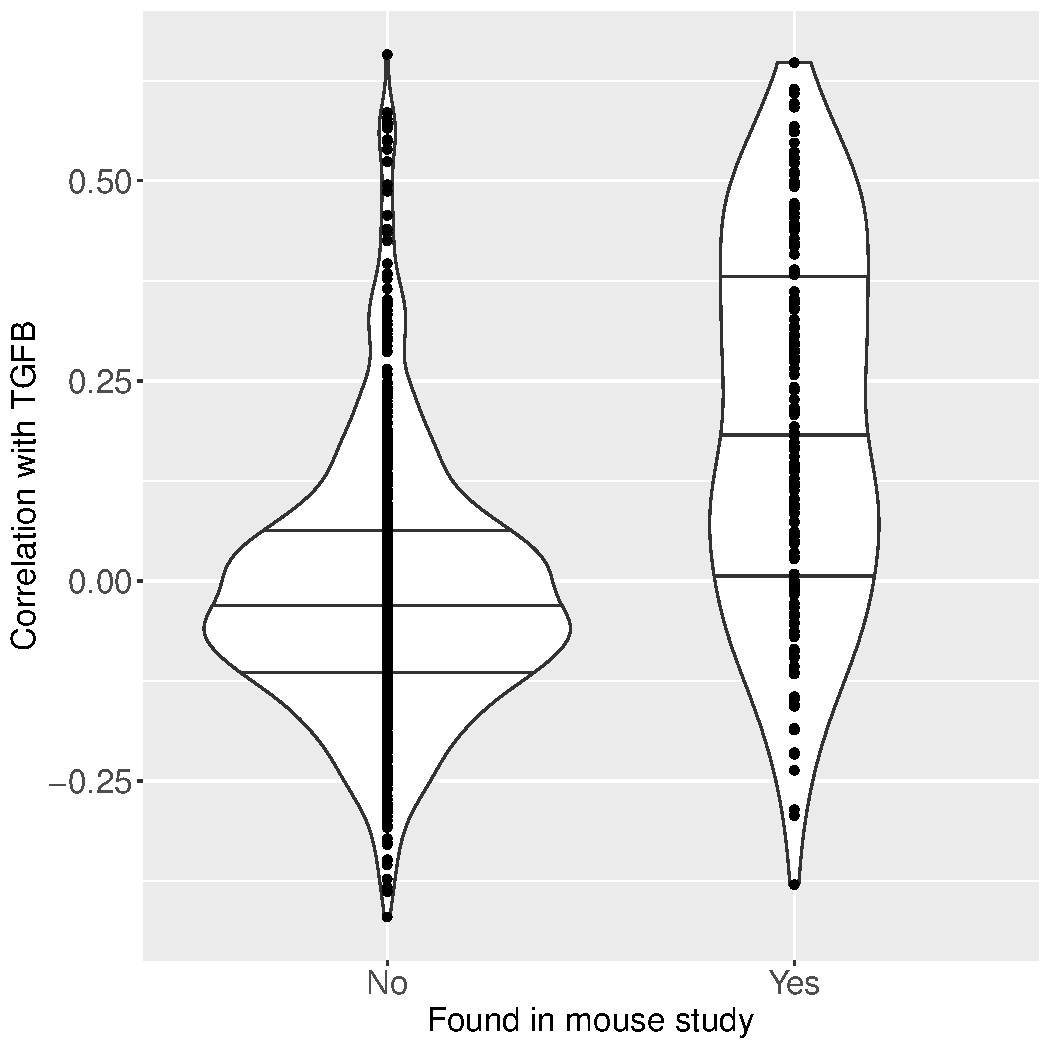
\includegraphics[width=0.6\textwidth]{images/tgfb_cor.pdf} 
% \end{center}
% \caption{TGFB data. Marginal correlations with the outcome vs. gene being in/out the mouse list}
% \label{fig:tgfb_exploratory}
% \end{figure}

\subsection{Adaptive informed selector}\label{sec:simulationsss}

We simulate data
%We compare the performance of $\hat S^{A,ei}$ to that of uninformed standard selection methods on data simulated 
from the linear model \eqref{eq:linearmodel} with standard Gaussian errors ($\sigma^2=1$), sample size $n \in [20,700]$, %varying from 20 to 700, 
and variable values drawn from a multivariate Gaussian with zero means, unit variances, and pairwise correlations $\mbox{cor}(x_{ij}, x_{il})= 0.5$ for $j \neq l$.

\begin{table*}[ht]
\caption{Sparsity and block assumptions in Examples 1--3}
\label{tab:examples_bis}
\begin{center}
\begin{tabular}[]{@{}cccccccc@{}}
\hline
Example & $p-s$ & $s$ & $s_1/p_1$ & $s_2/p_2$ & $\beta_{\min,1}^*$ & $\beta_{\min,2}^*=\beta_{\min}^*$ \\
\hline
$1$    & $3n/2$ & $3\ln(n)$ & $O(n^{-1}\ln(n))$ & $O(n^{-1/2}\ln(n))$  & 0.5 & 0.33\\
$2$    & $n$ & $3\ln(n)$ & $O(n^{-1}\ln(n))$ & $2/3$   & 0.5 & 0.33 \\
$3$    & $n$ & $3\ln(n)$ & $O(n^{-1}\ln(n))$ & $O(n^{-1}\ln(n))$  & 0.5 & 0.5\\
\hline
\end{tabular}
\end{center}
\end{table*}

% \david{Below we mention examples 1-4 but there's only examples 1-3. I always have a bit of a hard time following the description, I confess. Can we report $s_j/p_j$ and focus the discussion on that, even if not fully accurate it'd be easier to understand.}\paul{changed}
We consider three different examples with varying assumptions on the sparsity and informativeness of the external information summarized in Table~\ref{tab:examples_bis}. In Examples 1 and 2, external information is discriminative as it singles out a block $B_2$ that is less sparse than block $B_1$. In Example 1 the blocks are moderately discriminative, in that $(s_1/p_1)/(s_2/p_2)$ is a power of $n$. In Example 2 they are highly discriminative in that $\bbeta^*$ is sparse overall, but it is non-sparse within block 2 ($s_2 > p_2 - s_2)$. Example 3 is a non-discriminative average random guess where each block has half of the inactive parameters. The nonzero regression parameters $\beta_i^*$, $i\in S$, are set uniformly spaced in $(1/2, 1)$ except for one parameter in each block, which take values $\beta_{\min,1}^*$ and $\beta_{\min,2}^*$ in the last two columns of Table~\ref{tab:examples_bis}.
%DAVID: I commented out the discussion below because it confused me more than helped. Let's keep it short and simple.
%Examples 1, and 2 are discriminative settings, and then we set $\beta_{\min,1}^*>\beta_{\min,2}^*=\beta_{\min}^*$.In the non-discriminative setting of Example 4, we set $\beta_{\min,1}^*=\beta_{\min,2}^*$.


\begin{figure}[ht]
\begin{tabular}{M{49mm}M{49mm}M{49mm}}
        Ex.1 Prob. recovery& Ex.2 Prob. recovery & Ex.3 Prob. recovery\\
         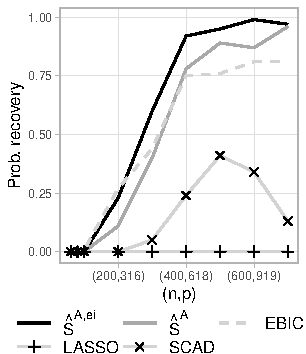
\includegraphics{images/p.probrecov.ex1.pdf} & 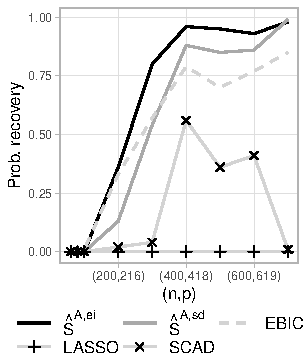
\includegraphics{images/p.probrecov.ex3.pdf} & 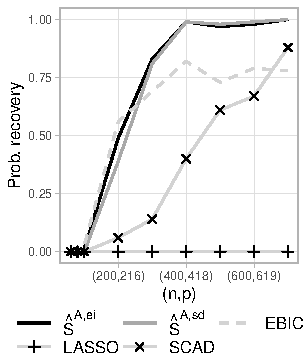
\includegraphics{images/p.probrecov.ex4.pdf}
\end{tabular}
\caption{Probability of correct selection with $\hat S^{ei}$, $\hat S^{A,sd}$, EBIC, LASSO and SCAD in Example 1 (left), 2 (middle), 3 (right).}
\label{fig:linregprobrec}
\end{figure}

\begin{figure}[ht]
\begin{tabular}{M{49mm}M{49mm}M{49mm}}
         Ex.2 FDR& Ex.2 Power & Ex.2 Est. MSE\\
         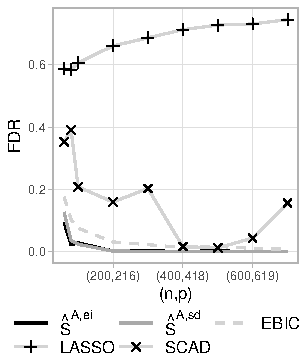
\includegraphics{images/p.FDR.ex3.pdf}  & 
         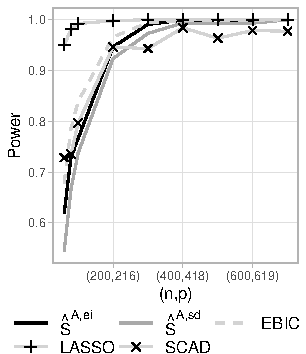
\includegraphics{images/p.power.ex3.pdf} & 
         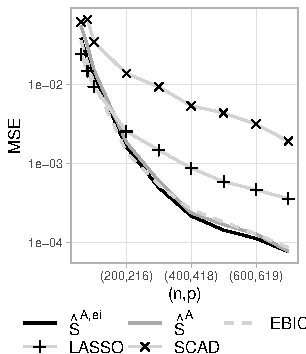
\includegraphics{images/p.est.mse.ex3.pdf} 
\end{tabular}
\caption{FDR (left), power (middle) and estimation MSE (right) with $\hat S^{A,ei}$, $\hat S^{A,sd}$, EBIC, LASSO and SCAD in Example 2.}
\label{fig:linregfdrpowmse}
\end{figure}

%\david{I'm confused. At the start of the section we distinguish between block penalties and the transello algorithm. Now Fig 1 is about transello when I thought it would be about the block algorithm. Why are we distinguishing block vs. transello? The figure is very nice though. :-)}\paul{There was a mistake in the caption. Corrected now. It is $\hat S^{A,ei}$, not transello}
For each sample size, we generate 100 datasets and report in Figure~\ref{fig:linregprobrec} the empirical probability of correct recovery for $\hat S^{A,ei}$, $\hat S^{A,sd}$, EBIC, LASSO and SCAD. In Examples 1 and 2 where blocks are discriminative, $\hat S^{A,ei}$ outperforms $\hat S^{A,sd}$ and performs similarly to the EBIC for small $n$. For large $n$, $\hat S^{A,ei}$ outperforms the EBIC and performs similarly to $\hat S^{A,sd}$. In the non discriminative block setting of Example 4, $\hat S^{A,ei}$ performs very similarly to $\hat S^{A,sd}$. LASSO and SCAD have consistently lower probability of recovery than the $\ell_0$ methods. The average false discovery rate (FDR) and power in Example 3 reported in Figure~\ref{fig:linregfdrpowmse} shed light on those differences. Compared to the uninformed $\hat S^{A,sd}$, our informed $\hat S^{A,ei}$ has equally low FDR but higher power. LASSO and EBIC have higher power than $\hat S^{A,ei}$ but higher FDR. In terms of mean squared error, $\hat S^{A,ei}$, $\hat S^{A,sd}$ and EBIC perform similarly and better than SCAD and LASSO.
Similar findings are observed in the other examples, and the corresponding plots can be found in Supplement XXX. We also report in Supplement XXX the average computation time to obtain $\hat{S}^{A,b}$ as a function of dimension $p$. In all three examples, the average time does not exceed 20 seconds.


% \begin{figure}[ht]
% \begin{minipage}{1\columnwidth}
% \begin{tabular}{M{75mm}M{75mm}}
%         Example 1& Example 3\\
%          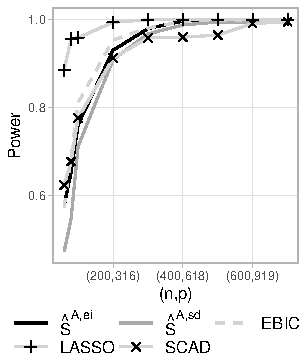
\includegraphics[scale=1]{images/p.power.ex1.pdf} & 
%          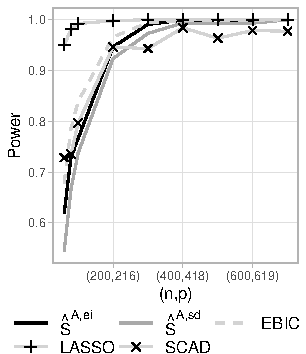
\includegraphics[scale=1]{images/p.power.ex3.pdf} \\ 
%          Example 4& Example 5\\
%          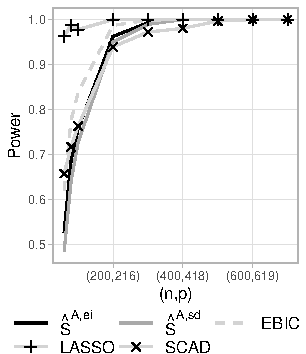
\includegraphics[scale=1]{images/p.power.ex4.pdf}  & 
%          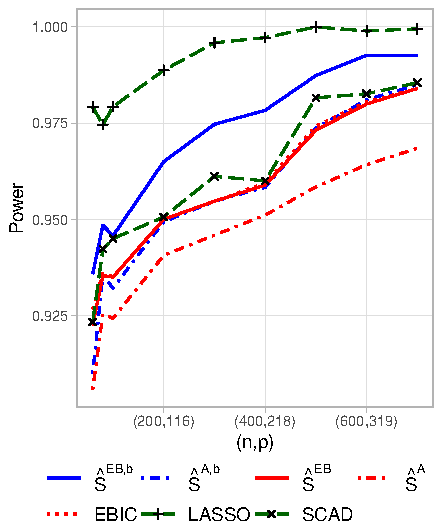
\includegraphics[scale=1]{images/p.power.ex5.pdf} 
% \end{tabular}
% \end{minipage}
% \caption{Power with $\hat S^{EB,b}$, $\hat S^{A,ei}$, $\hat S^{EB}$, $\hat S^{A,sd}$, EBIC, LASSO and SCAD in Example 1 (top left), 2 (top right), 4 (bottom left) and 5 (bottom right).}
% \label{fig:linregpower}
% \end{figure}

% \begin{figure}[ht]
% \begin{minipage}{1\columnwidth}
% \begin{tabular}{M{75mm}M{75mm}}
%         Example 1& Example 3\\
%          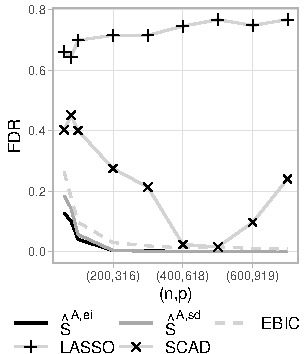
\includegraphics[scale=1]{images/p.FDR.ex1.pdf} & 
%          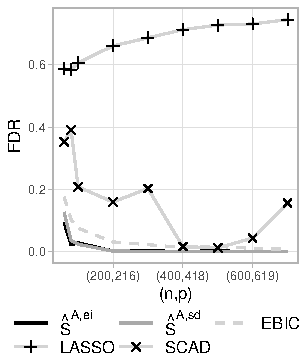
\includegraphics[scale=1]{images/p.FDR.ex3.pdf} \\ 
%          Example 4& Example 5\\
%          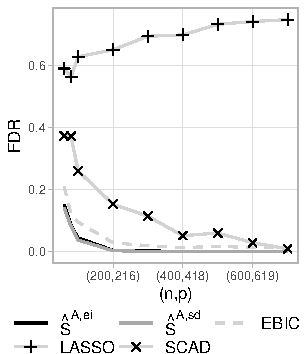
\includegraphics[scale=1]{images/p.FDR.ex4.pdf}  & 
%          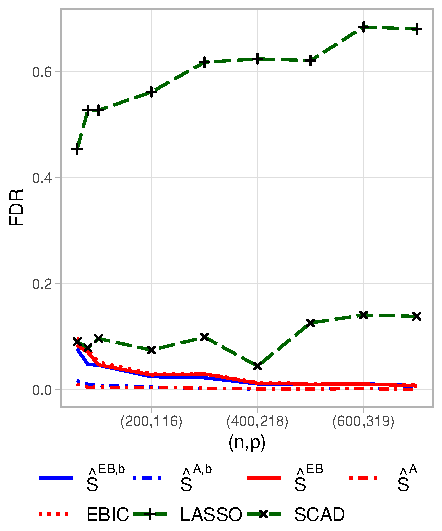
\includegraphics[scale=1]{images/p.FDR.ex5.pdf} 
% \end{tabular}
% \end{minipage}
% \caption{False discovery rate with $\hat S^{EB,b}$, $\hat S^{A,ei}$, $\hat S^{EB}$, $\hat S^{A,sd}$, EBIC, LASSO and SCAD in Example 1 (top left), 2 (top right), 4 (bottom left) and 5 (bottom right).}
% \label{fig:linregfdr}
% \end{figure}

% \begin{figure}[ht]
% \begin{minipage}{1\columnwidth}
% \begin{tabular}{M{75mm}M{75mm}}
%         Example 1& Example 3\\
%          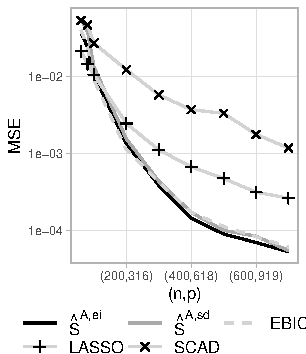
\includegraphics[scale=1]{images/p.est.mse.ex1.pdf} & 
%          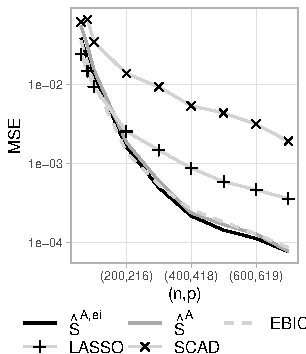
\includegraphics[scale=1]{images/p.est.mse.ex3.pdf} \\ 
%          Example 4& Example 5\\
%          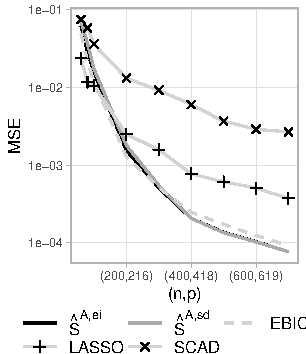
\includegraphics[scale=1]{images/p.est.mse.ex4.pdf}  & 
%          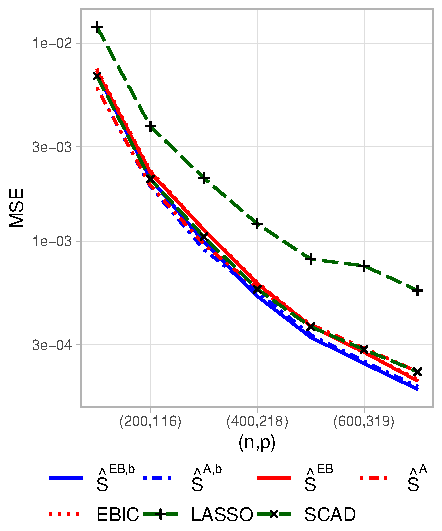
\includegraphics[scale=1]{images/p.est.mse.ex5.pdf} 
% \end{tabular}
% \end{minipage}
% \caption{Mean squared error (on a log scale) in coefficient estimation with $\hat S^{EB,b}$, $\hat S^{A,ei}$, $\hat S^{EB}$, $\hat S^{A,sd}$, EBIC, LASSO and SCAD in Example 1 (top left), 2 (top right), 4 (bottom left) and 5 (bottom right).}
% \label{fig:linregmse}
% \end{figure}

% \begin{figure}[ht]
% \begin{minipage}{1\columnwidth}
% \begin{tabular}{M{75mm}M{75mm}}
%         Example 1& Example 3\\
%          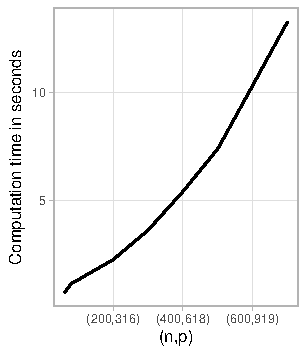
\includegraphics[scale=1]{images/p.time.ex1.pdf} & 
%          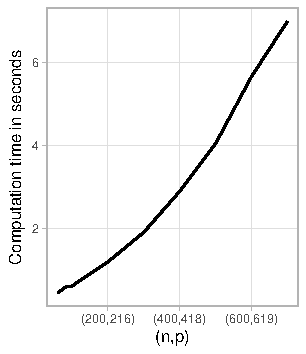
\includegraphics[scale=1]{images/p.time.ex3.pdf} \\ 
%          Example 4& Example 5\\
%          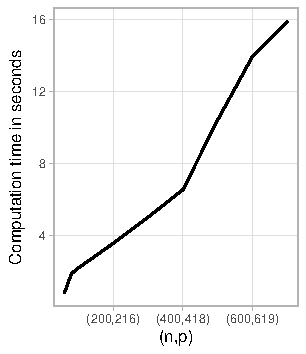
\includegraphics[scale=1]{images/p.time.ex4.pdf}  & 
%          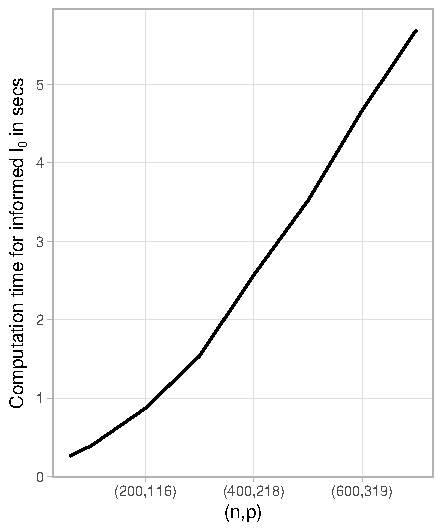
\includegraphics[scale=1]{images/p.time.ex5.pdf} 
% \end{tabular}
% \end{minipage}
% \caption{Computation time in seconds to obtain $\hat{S}^{EB,b}$ and $\hat{S}^{A,b}$ in Example 1 (top left), 2 (top right), 4 (bottom left) and 5 (bottom right).}
% \label{fig:linregtime}
% \end{figure}

%The plots of the average power and FDR in Figures~\ref{fig:linregpower} and~\ref{fig:linregfdr} explain the differences in the probability of recovery. They show that, in discriminative examples, the block empirical Bayes selector $\hat S^{EB,b}$ and the block adaptive selector $\hat S^{A,ei}$ have more power than their uninformed counterparts $\hat S^{EB}$ and $\hat S^{A,sd}$ respectively, but similar FDR. In the non-discriminative Example 5, the FDR is also similar but the increase power is nearly 0. Using external information, the proposed procedure is able to increase the power without making sacrifices in the control of false positives. The small or nearly 0 probability recovery of LASSO and SCAD is explained by high power but high FDR in the case of LASSO and, in the case of SCAD rather low FDR but low power. The FDR of SCAD is still larger than that of informed and uninformed penalties in most cases.

%In terms of mean squared error in coefficient estimation, informed $\hat S^{EB,b}$ and $\hat S^{A,ei}$ perform similarly to the uninformed $\hat S^{EB}$ and $\hat S^{A,sd}$. In Examples 1, 3 and 4, $\hat S^{EB,b}$ and $\hat S^{A,ei}$ have a similar or slightly smaller error than LASSO and a clearly smaller error than SCAD. In Example 5, $\hat S^{EB,b}$ and $\hat S^{A,ei}$ perform similarly to SCAD but better than LASSO. 


\subsection{Tran-s-ell0 algorithm}\label{sec:TLexample}

\begin{figure}[ht]
\begin{tabular}{M{52mm}M{52mm}M{52mm}}
         Scenario 1, $h=0$& Scenario 2, $h=0.4$ & Scenario 3, $h=1$\\
         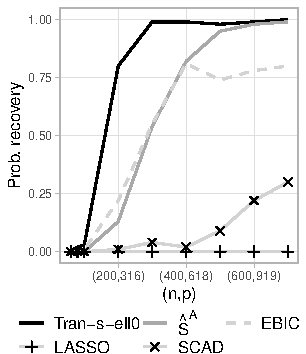
\includegraphics{images/p.TL.probrecov.ex1.pdf} &          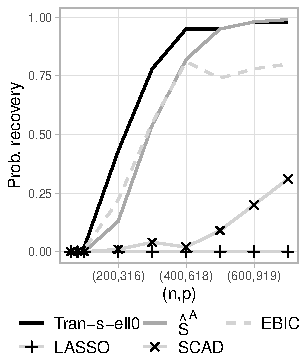
\includegraphics{images/p.TL.probrecov.ex3.pdf} &      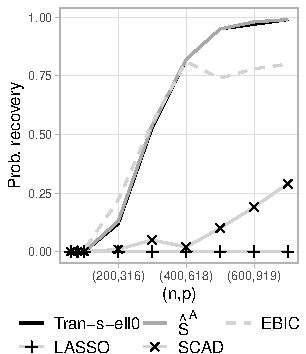
\includegraphics{images/p.TL.probrecov.ex5.pdf} 
\end{tabular}
\caption{Probability of correct selection with Tran-s-ell0 algorithm, $\hat S^{A,sd}$, EBIC, LASSO and SCAD in Example 1 (left), 2 (middle), 3 (right).}
\label{fig:TLpr}
\end{figure}

We apply next the \hyperlink{lab:AlgoTL}{Tran-s-ell0 algorithm} to simulated data where the target sample sizes $n$ ranges from 20 to 700. For each sample size, we generate 100 sets of target and source datasets. In each target dataset, a data-generating $\bbeta^*$ is drawn such that $p-s=3n/2$, $s=3\ln(n)$, and nonzero coefficients are uniformly spaced in $(1/3,1)$. Variable values are drawn from a multivariate Gaussian with zero means, unit variances, and pairwise correlations $\mbox{cor}(x_{ij}, x_{il})= 0.5$ for $j \neq l$. For each target dataset, we generate two source datasets with sample size 700 and data-generating parameters that are equal to the target $\bbeta^*$ where a proportion $h$ of the nonzero target coefficients is set to 0 and an equal number of the zero target coefficients is set uniformly spaced in $(1/3,1)$. Source variable are drawn from the same multivariate Gaussian distribution as in the target data. The Hamming distance between the indicator vectors of active variables in the source and target data is then $2hs$. We select variables in the source datasets with a standard $\ell_0$ penalty $\kappa=\tfrac12\ln(n)+\ln(p)$ and feed the selected sets to \hyperlink{lab:AlgoTL}{Tran-s-ell0}. We consider three scenarios and report the average probability of recovery in Figure~\ref{fig:TLpr}. In Scenario 1, the source and target sets of active variables are the same, that is $h=0$. In Scenario 2, the source and target sets of active variables are similar but different with $h=0.4$. Scenario 3 is an example of completely irrelevant transfer where $h=1$. In Scenario 1 and 2, \hyperlink{lab:AlgoTL}{Tran-s-ell0 algorithm} outperforms all the other selectors. In Scenario 3, $\hat S^{A,ei}$ performs similarly to $\hat S^{A,sd}$, better than LASSO and SCAD, slightly worse than EBIC for small $n$ but signficantly better for large $n$.  \paul{This is the simulation I initially did. But now I think I should EITHER only simulate sets of variables selected on the sources OR change the source designs to stress our point on the absence of requirement on the similarity of the designs}.

Next, we apply \hyperlink{lab:AlgoTL}{Tran-s-ell0} to a biological data set. In molecular biology, it is common to use animal models (e.g. mice) to study genomic mechanisms such as gene expression. Findings from such studies often serve as a basis to study human diseases, for example, to assess whether genes that played key roles in the animal model are also important in humans. Specifically, \cite{calon:2012} compared mice where gene TGFB was silenced to mice where it was not, showed that TGFB plays a crucial role in colon cancer progression, and found a list of 172 genes that were associated with TGFB. We use \hyperlink{lab:AlgoTL}{Tran-s-ell0 algorithm} to leverage this set of 172 genes in the selection of genes associated to TGFB in a colon cancer dataset of $n=262$ human samples analyzed in~\cite{rossell:2017}. We regress TGFB expression on that of $p=1000$ genes. All variables are standardized to zero mean and unit variance. In this dataset, obtaining $\hat S^{A,ei}$ in Step 2 of \hyperlink{lab:AlgoTL}{Tran-s-ell0 algorithm} took 49 seconds. 

%\david{We should elaborate on the discussion of results below. A priori there's no reason why our findings are better than those from the EBIC. Can we argue based on the known roles of the identified genes, as we did in the other paper? Or show the differences in the pseudo-posterior probabilities, it might be that we get them to be closer to 1 for genes in the mouse list -- as in our other paper. That is it's not just about selection/not selection, but also about the evidence in favor of the selection.}
Table~\ref{tab:selgenes} reports the genes selected with \hyperlink{lab:AlgoTL}{Tran-s-ell0}, $\hat S^{A,sd}$, EBIC, LASSO and SCAD. Compared to the uninformed counterpart $\hat{S}^{A,sd}$ \hyperlink{lab:AlgoTL}{Tran-s-ell0} focuses discoveries on the genes that were found to be associated to TGFB in mice: it selects more genes from the mouse list, and less genes from outside the list. LASSO and SCAD select a much larger number of genes than the informed and uninformed $\ell_0$ penalties. Given the higher levels of false discovery rates that these $\ell_1$ methods typically exhibit in correlated design \citep{slope}, those extra discoveries should be considered with caution. EBIC selects the same genes as our algorithm in the mouse list, but more genes outside of the mouse list. Finally, the EBIC selects the same genes from the mouse list as \hyperlink{lab:AlgoTL}{Tran-s-ell0} but also three more genes from outside the list. In our simulations, EBIC had larger FDR but larger power than our informed selector for small sample size as here. Then, to further assess relevance of those extra discoveries and the quality of the models selected by EBIC and \hyperlink{lab:AlgoTL}{Tran-s-ell0}, we computed and report in Table~\ref{tab:cvmse.pseudoprob} the associated cross-validated mean squared error in estimation and some pseudo-posterior inclusion probabilities, $p(\beta_i)=\sum_{\M} NC(M)I(i\in M)$.

\begin{table*}[ht]
\caption{Selected genes in each block}
\label{tab:selgenes}
\centering
\begin{tabular}{lC{0.1\linewidth}C{0.22\linewidth}C{0.1\linewidth}C{0.22\linewidth}}
\hline
 & \multicolumn{2}{c}{In mouse list} & \multicolumn{2}{c}{Outside of mouse list} \\ [3pt] \cline{2-5} 
 Method & \multicolumn{1}{C{0.15\linewidth}}{Number of discoveries} & Genes & \multicolumn{1}{C{0.15\linewidth}}{Number of discoveries} & Genes\\ 
\hline
Tran-s-ell0 & \multicolumn{1}{C{0.1\linewidth}}{4} & ESM1, GAS1, HIC1, CILP & \multicolumn{1}{C{0.1\linewidth}}{0} & - \\
\hline
$\hat S^{A,sd}$ & \multicolumn{1}{C{0.1\linewidth}}{2} & IGFBP3, CILP & \multicolumn{1}{C{0.1\linewidth}}{2} & LGALS1, ARHGEF1  \\
\hline
EBIC & \multicolumn{1}{C{0.1\linewidth}}{4} &  ESM1, GAS1, HIC1, CILP & \multicolumn{1}{C{0.1\linewidth}}{3} & KCNJ5-AS1, ZBTB46, OXER1 \\
\hline
LASSO& \multicolumn{1}{C{0.1\linewidth}}{22} & GAS1, HIC1, IGFBP3, CILP, DNAJB5, \ldots & \multicolumn{1}{C{0.1\linewidth}}{55} &  KCNJ5-AS1, ZBTB46, OXER1, LGALS1, \ldots \\
\hline
SCAD & \multicolumn{1}{C{0.1\linewidth}}{11} & GAS1, HIC1, IGFBP3, CILP, DNAJB5, \ldots & \multicolumn{1}{C{0.1\linewidth}}{5} &  POLQ, CRIP2, ZBTB46, VSIG4, LGALS1 \\
\hline
\end{tabular}
\end{table*}

\begin{table*}[ht]
\caption{$\hat S^{A,sd}$ vs EBIC: cross-valitated MSE and pseudo-posterior probabilities}
\label{tab:cvmse.pseudoprob}
\centering
\begin{tabular}{lccccc}
\hline
 & & \multicolumn{4}{c}{Pseudo-posterior probabilities}  \\[3pt] \cline{3-6} 
 Method & CV-MSE & ESM1 & GAS1 & HIC1 & CILP\\ 
\hline
EBIC & 0.54& 0.55 & 0.88 & 0.81 & 0.95\\
\hline
Tran-s-ell0 & 0.49 & 0.74 & 0.90 & 0.95 & 0.99\\
\hline
\end{tabular}
\end{table*}

\section{Discussion}
We discussed how variable selection properties can be improved by leveraging external information on the likelihood of variables to be truly associated to the outcomes. We first analyzed the gains achievable by an oracle ideal selector, providing a benchmark for future concrete selection methods. We proposed then a data-based selector that recovers most of the benefits of the oracle selector. As a particular case, we introduced a flexible and robust transfer learning algorithm where the set of
variables selected in source datasets is transferred to ease variable selection in a target dataset. 

A question for future work is to understand the benefits of leveraging external information and the transfer of selected variables in estimation. Our simulations suggest that improvements can be achieved, but we have not discussed related theory and estimation procedures. This work also focused on external information in variable selection in linear regression. The benefits of incorporating external information and how to make them a reality in other structural learning problems like graphical model selection is another interesting research avenue.


\bibliography{references.bib}

\phantomsection\label{supplementary-material}
\bigskip

\begin{center}

{\large\bf SUPPLEMENTARY MATERIAL}

\end{center}

\renewcommand{\theequation}{S.\arabic{equation}}

\begin{description}
\item[Tightness of conditions for variable selection consistency in linear regression:]
comparison of our sufficient and necessary conditions of Section~\ref{sec:properties_legression} applied to standard $\ell_0$ penalties to results in literature.
\item[Examples of benefits of $\hat S^{ei}$:]
Illustrations in four examples of sparsity and informativeness of the blocks of the benefits of $\hat S^{ei}$ in oracle selection properties.
\item[Complementary material on numerical illustrations:]
Reports of false discovery rates, power, mean squared error and computation time in the numerical illustrations of the performance of $\hat S^{ei}$ and Tran-s-ell0.
\item[Proofs]
\end{description}

\section{Limits on variable selection consistency in linear regression with standard (non-informed) selectors}\label{suppsec:tightness}


Sufficient and necessary assumptions for variable selection consistency in \eqref{eq:linearmodel} under correlated random designs for a (non-informed) oracle selector that knows $s$ were derived by \cite{infotheowainwright} and \cite{wang2010}. We compare those to our assumptions for the standard $\ell_0$ selector $\hat{S}^{sd}$. Specifically, we compare the scaling of $n$ implied by the assumptions under six regimes of interest of $\left(p, s, \beta_{\min }^*\right)$. For simplicity, the effect of the conditioning of $\bX$ is ignored, i.e $\rho(\bX)$, $\bar{\lambda}$ and $\underline{\lambda}$ are considered fixed and bounded away from 0. \cite{infotheowainwright} and \cite{wang2010} derive sufficient and necessary assumptions in a setting that slightly differs from the one considered here. They study a slightly weaker notion of consistency and necessary conditions are given for the harder task of recovering $S$ when the latter is chosen uniformly at random among subsets of size $s$. Although their assumptions and ours are then not entirely comparable, the comparison gives an idea of the tightness of our results.

Theorem~\ref{theo:suffcondlinearmodel} shows variable selection consistency with $\hat{S}^{sd}$ under Assumptions~\hyperlink{lab:A4}{A4} and \hyperlink{lab:A5}{A5}. By \eqref{eq:gpkr} in the proof of Theorem~\ref{prop:fullrecovreg}, an assumption slightly less stringent than \hyperlink{lab:A5}{A5}, and easier to analyse, is sufficient together with \hyperlink{lab:A4}{A4}. That assumption is: \\[5pt]
for each block $j$, there exists $g_j\to \infty$ such that for every sufficiently large $n$,
    \begin{equation}\label{eq:newasssufflinreg}
        \frac{(1-\gamma) n\rho(\bX)}{6}{\beta_{\min,j}^*}^2 \,- \,\kappa_j \;=\; \ln(s_j) + g_j.
    \end{equation}
where $\gamma:=\tfrac12(1+\max_j\ln(p_j-s_j)/\kappa_j)\in (\tfrac12,1)$

Consider assumptions~\hyperlink{lab:A5}{A5} and \hyperlink{lab:A4}{A4} for the standard $\ell_0$ selector $\hat{S}^{sd}$ with single penalty $\kappa$. Their combination implies an assumption on the scaling of $(n,p,s,\beta_{\min}^*)$. To simplify the analysis of that assumption, we assume $\kappa=(1+\varepsilon)\ln(p-s)$ for some fixed $\varepsilon>0$. This choice guarantees that $\kappa$ meets assumption~\hyperlink{lab:A4}{A4} and that $1-\gamma$ is constant and bounded away from 0. A sufficient assumption on $(n,p,s,\beta_{\min}^*)$ that follows from assumptions~\hyperlink{lab:A5}{A5} and \eqref{eq:newasssufflinreg} is then that there exists $t\to \infty$, growing at an arbitrarily slow rate, such that:
\begin{equation}\label{eq:groh}
    n= \frac{12(1+\varepsilon)}{\varepsilon}\frac{(1+\varepsilon)\ln(p-s)+\ln(s)}{\rho(\bX){\beta_{\min}^*}^2} \;+\;t
\end{equation}

Theorem 1 in \cite{infotheowainwright} shows a sufficient assumption on $(n,p,s,\beta_{\min}^*)$ for the optimal selector that knows $s$ to be variable selection consistent in random Gaussian designs is:
\begin{equation}\label{eq:groh2}
    n > (c_1+2048) \max \left\{\log \binom{p-s}{s}, \frac{\log (p-s)}{\rho(\bX) {\beta_{\min}^*}^2}\right\}
\end{equation}
for some $c_1 >0$. 

An immediate initial conclusion is that for any regime of $(n,p,s,\beta_{\min}^*)$ such that $\ln(s)=O({\beta_{\min}^*}^2)$, \eqref{eq:groh} is less stringent than \eqref{eq:groh2}. It is also the case when ${\beta_{\min}^*}^2=\Theta(1)$ and $s<p/2$. Table~\ref{tab:scalingsuff} gives, for six regimes of interest, the scalings of $n$ implied by \eqref{eq:groh} and \eqref{eq:groh2}. In regimes 1, 2 and 5 the scalings implied by our sufficient assumptions match those implied by the sufficient assumption of \cite{infotheowainwright}. Our assumption is tighter in regimes 3 and 6, with the difference being particularly large in regime 3. In that regime, results by \cite{infotheowainwright} imply a sample size growing linearly in the dimension, while our results shows a logarithmic growth in dimension is sufficient. In regime 4 where $s=o(p)$, our assumption is loser by a term of order $s\ln(s)$. Overall, our results refine the known limits on variable selection in the standard non-informed setting and show a well calibrated standard $\ell_0$ penalty performs as well as an optimal selector in the vast majority of regimes.

% \begin{table*}[ht]
% \center
% \caption{Scalings of sufficient assumptions for variable selection consistency\vspace{1em}}
% \label{tab:scalingsuff}
% \begin{tabular}{@{}ccccc@{}}
% \hline \\[-1em]
% \small{Regime} &  \thead{Sufficient assumption\\ in \cite{infotheowainwright}} & \thead{Our sufficient \\assumption} \\
% \hline\\[-1em]
% 1.\thead{$s=\Theta(p)$\\${\beta_{\min}^*}^2=\Theta(1/s)$}    & $\Theta(p\ln(p))$  & $\Theta(p\ln(p))$ \\\hline\\[-1em]
% 2.\thead{$s=\Theta(p)$\\${\beta_{\min}^*}^2=\Theta\big(\ln(s)/s\big)$}  & $\Theta(p)$  & $\Theta(p)$ \\\hline\\[-1em]
% 3.\thead{$s=\Theta(p)$\\${\beta_{\min}^*}^2=\Theta(1)$}   & $\Theta(p)$ & $\Theta(\ln(p))$ \\\hline\\[-1em]
% 4.\thead{$s=o(p)$\\${\beta_{\min}^*}^2=\Theta(1/s)$}     & $\Theta(s\ln(p-s))$ & $\Theta(s\ln(p-s)+s\ln(s))$ \\\hline\\[-1em]
% 5.\thead{$s=o(p)$\\${\beta_{\min}^*}^2=\Theta(\ln(s)/s)$} & $\Theta\big(s\ln\big(p/s\big)\big)$ & $\Theta\big(s\ln\big(p/s\big)\big)$ \\\hline\\[-1em]
% 6.\thead{$s=o(p)$\\${\beta_{\min}^*}^2=\Theta(1)$} & $\Theta\big(s\ln(p/s)\big)$ & $\Theta(\ln(p-s))$  \\\hline
% \end{tabular}
% \end{table*}


In this thesis we establish the necessity of assumption~\eqref{eq:betaminnecreg} which, when applied to $\hat{S}^{sd}$ ($\hat{S}^{ei}$ with $b=1$), implies
\begin{equation}\label{eq:gpiR}
\lim_{n\to\infty}\sqrt{n\bar{\lambda}}\beta_{\min}^*-\underline{\lambda}\sqrt{\ln(p-s)} n\;=\; \frac{\underline{\lambda}\sqrt{\ln(p-s)}}{\bar{\lambda}{\beta_{\min}^*}^2}+t^{\prime}
\end{equation}
where $t^{\prime} \to\infty$ and $1/t = o({\beta_{\min}^*}^2)$. In other words, $t$ must grow faster than ${\beta_{\min}^*}^2$ shrinks. For comparison, Theorem 1 in \cite{wang2010} gives, for the \textit{harder} problem of recovering $S$ when $S$ is chosen at random in $\M$, the necessary assumption 
\begin{equation}\label{eq:gpiR2}
n>\max \left\{f_1(p, s, \lambda), \ldots, f_k(p, s, \lambda), s\right\}
\end{equation}
where
$$
f_m(p, s, \lambda):=\frac{\ln \binom{p-s+m}{m}-1}{\frac{1}{2} \ln \left(1+m \beta_{\min,j}^2\left(1-\frac{m}{p-s+m}\right)\right)}\quad\text{for}\;\;m=1, \ldots, s
$$
Table~\ref{tab:scalingnec} gives, for six regimes of interest, the scalings of $n$ implied by \eqref{eq:gpiR} and \eqref{eq:gpiR2}. 
% \begin{table*}[ht]
% \center
% \caption{Scalings of necessary assumptions for variable selection consistency \vspace{1em}}
% \label{tab:scalingnec}
% \begin{tabular}{@{}ccccc@{}}
% \hline \\[-1em]
% \small{Regime}  & \thead{Necessary assumption\\ in \cite{wang2010}}  & \thead{Our necessary \\assumption}\\
% \hline\\[-1em]
% 1. \thead{$s=\Theta(p)$\\${\beta_{\min}^*}^2=\Theta(1/s)$}    & $\Theta(p\ln(p))$ & $\Theta(p\ln(p))$ \\\hline\\[-1em]
% 2.\thead{$s=\Theta(p)$\\${\beta_{\min}^*}^2=\Theta\big(\ln(s)/s\big)$}   & $\Theta(p)$ & $\Theta(p)$ \\\hline\\[-1em]
% 3.\thead{$s=\Theta(p)$\\${\beta_{\min}^*}^2=\Theta(1)$}  &  $\Theta(p)$ & $\Theta(\ln(p))$ \\\hline\\[-1em]
% 4.\thead{$s=o(p)$\\${\beta_{\min}^*}^2=\Theta(1/s)$}     & $\Theta(s\ln(p-s))$  & $\Theta(s\ln(p-s))$\\\hline\\[-1em]
% 5.\thead{$s=o(p)$\\${\beta_{\min}^*}^2=\Theta(\ln(s)/s)$} & $\max \Big\{ \Theta\Big(\tfrac{s\ln(p/s)}{\ln(\ln(s))}\Big), \Theta\Big(\tfrac{s\ln(p-s)}{\ln(s)}\Big) \Big\}$ &$\Theta\big(s\ln\big(p/s\big)\big)$ \\\hline\\[-1em]
% 6.\thead{$s=o(p)$\\${\beta_{\min}^*}^2=\Theta(1)$} & {$\max \Big\{\Theta\Big(\tfrac{s\ln(p/s)}{\ln(s)}\Big), \Theta(s) \Big\}$} & $\Theta(\ln(p-s)+\ln(s))$ \\\hline
% \end{tabular}
% \end{table*}

Observe first that the scalings implied by our necessary assumption match those implied by our sufficient assumption in all regimes but 4 and 6. In regimes 4 and 6, where $s=o(p)$, our sufficient assumption is stricter by linear and logarithmic terms in the sparsity $s$. In regimes 1, 2 and 4, the scalings implied by our necessary assumption and that of \cite{wang2010} match. In regime 5, our necessary assumption is tighter than that of \cite{wang2010}. In regimes 3 and 6, the necessary assumptions of \cite{wang2010} are stricter than mine and also stricter than our sufficient assumption. This may be explained by the harder nature of the recovery problem considered by \cite{wang2010}. 

\section{Examples of benefits of $\hat S^{ei}$}
We illustrate here the benefits of $\hat S^{ei}$ over $\hat S^{sd}$ with four concrete examples contemplating different scenarios of sparsity regimes and informativeness of the blocks, summarized in Table~\ref{tab:examples}. We assume an orthonormal design such that $\rho(\bX)=1$ for simplicity and focus on a sparse setting where $\ln(s)=o(\ln(p-s))$, with two blocks ($b=2$). The smallest non-zero $|\beta_i^*|$, $\beta_{\min}^*$ is assumed to be located in block $2$, without loss of generality. 

\begin{table*}[ht]
\caption{Sparsity and block assumptions in Examples 1--4}
\label{tab:examples}
\begin{center}
\begin{tabular}[]{@{}cccccc@{}}
\hline
Example & $p-s$ & $p_1-s_1$ & $p_2-s_2$ & $s_1$ 
& $s_2$\\
\hline
$1$    & $3n/2$ & $3n/2-\sqrt{n}$ & $\sqrt{n}$  & $3\ln(n)/2$  & $3\ln(n)/2$ \\
$2$    & $e^{n/20}$ & $e^{n/20}-n^2$ & $n^2$  & $3\ln(n)/2$  & $3\ln(n)/2$   \\
$3$    & $n$ & $n-\ln(n)$ & $\ln(n)$  & $3\ln(n)/2$  & $3\ln(n)/2$   \\
$4$    & $n$ & $n/2$ & $n/2$  & $3\ln(n)/2$  & $3\ln(n)/2$\\
\hline
\end{tabular}
\end{center}
\end{table*}

In Examples 1 to 3, external information is discriminative as it singles out a block $B_1$ that is sparser than block $B_2$. In Example 1 the blocks are moderately discriminative, in that $(p_1-s_1)/(p_2-s_2)$ is a power of $n$. In Example 2 they are highly discriminative, since $(p_1-s_1)/(p_2-s_2)$ is exponential in $n$ and in Example 3 they are highly discriminative in that $\bbeta^*$ is sparse overall, but it is non-sparse within block 2 ($s_2 > p_2 - s_2)$. Example 4 is a non-discriminative random guess where each block has half of the inactive parameters. 

Figures~\ref{fig:boundthresh} and~\ref{fig:boundthresh2} plot the ranges of penalty values $\kappa$ and $(\kappa_1,\kappa_2)$ ensuring selection consistency with $\hat{S}^{sd}$ and $\hat{S}^{ei}$ given in \eqref{eq:rangethreshex} and \eqref{eq:rangeblockthreshex} in the four examples, assuming $\beta^*_{\min,1}=2/3$, $\beta^*_{\min,2}=\beta^*_{\min}=1/10$, $f=g=\ln(ln(n))$ and $f_j=g_j=\ln(ln(n))$ for all $j$. In Example 2, asymptotic recovery with $\hat{S}^{sd}$ is not possible in the range of values of $n$ considered while it is with $\hat{S}^{ei}$.
In the other examples, asymptotic recovery with $\hat{S}^{sd}$ is possible, but it requires larger $n$ than with $\hat{S}^{ei}$. Example 1 shows that the gain can be large even when blocks are moderately discriminative, and Example 3 when some blocks are non-sparse.
The gain in terms of the value of $n$ making recovery possible  is close to null in Example 4 when external information is non-discriminative. 

% \begin{figure}[ht]
% \centering
% \begin{minipage}{1\columnwidth}
% \setlength{\tabcolsep}{1pt}
% \centering
% \begin{tabular}{M{3mm}M{66mm}M{66mm}}
%        \toprule
%          & Example 1 & Example 2  \\
%         \midrule
%         $\kappa$ & 
\includegraphics[scale=1]{images/taus/p.scen1tau.pdf} & 
\includegraphics[scale=1]{images/taus/p.scen2tau.pdf} \\
%         $\kappa_1$ & 
\includegraphics[scale=1]{images/taus/p.scen1tau1.pdf} & 
\includegraphics[scale=1]{images/taus/p.scen2tau1.pdf}  \\
%         $\kappa_2$ & 
\includegraphics[scale=1]{images/taus/p.scen1tau2.pdf} & 
\includegraphics[scale=1]{images/taus/p.scen2tau2.pdf}  \\
%         \bottomrule
% \end{tabular}
% \setlength{\tabcolsep}{6pt}
% \end{minipage}
%     \caption{Smallest (dashed) and largest (solid) value of $\kappa$ leading to consistent model recovery in Examples 1 and 2, as given in \eqref{eq:rangethreshex} and \eqref{eq:rangeblockthreshex}. Grey indicates settings where the interval is empty}
%  \label{fig:boundthresh}
% \end{figure}

% \begin{figure}[ht]
% \centering
% \begin{minipage}{1\columnwidth}
% \centering
% \setlength{\tabcolsep}{1pt}
% \begin{tabular}{M{3mm}M{66mm}M{66mm}}
%        \toprule
%          & Example 3 & Example 4 \\
%         \midrule
%         $\kappa$ & 
\includegraphics[scale=1]{images/taus/p.scen3tau.pdf} & 
\includegraphics[scale=1]{images/taus/p.scen4tau.pdf} \\
%         $\kappa_1$ & 
\includegraphics[scale=1]{images/taus/p.scen3tau1.pdf} & 
\includegraphics[scale=1]{images/taus/p.scen4tau1.pdf} \\
%         $\kappa_2$ & 
\includegraphics[scale=1]{images/taus/p.scen3tau2.pdf} & 
\includegraphics[scale=1]{images/taus/p.scen4tau2.pdf} \\
%         \bottomrule
% \end{tabular}
% \setlength{\tabcolsep}{6pt}
% \end{minipage}
%     \caption{%Valid upper bound (solid) and lower bound (dashed) on $\tau$, $\tau_1$ and $\tau_2$ in Examples 1 to 4.
%     Smallest (dashed) and largest (solid) value of $\tau$ leading to consistent model recovery in Examples 3 and 4, as given in \eqref{eq:rangethreshex} and \eqref{eq:rangeblockthreshex}. Grey indicates settings where the interval is empty}
%  \label{fig:boundthresh2}
% \end{figure}

Figure~\ref{fig:ratios} plots the ratio ${OR}^{ei}/OR$ in \eqref{eq:goodoregratio} for Examples 1 to 3 where blocks are discriminative with $\gamma$ set to $3/4$ for simplicity. The smallest signals in each block are such that $\beta_{\min }^*=\beta_{\min,2}^*=1/5$ and $\beta_{\min,1}^*=1.3\beta_{\min }^*$ to guarantee the recovery is possible with both $\hat{S}^{sd}$ and $\hat S^b$. Figure~\ref{fig:ratios} shows that in the three examples, the convergence is much faster with $\hat S^b$. The more discriminative the blocks are, the larger the gain.
\paul{I have made simplifications assumptions on $\gamma$ in the discussions of the oracle convergence rates but in reality $\kappa^*$ depends on $\gamma$ and $\gamma$ depends on $\kappa^*$.}



\section{Proofs}\label{app:proofs}


Section~\ref{suppsec:auxiliary} presents results auxiliary to the rest of the proofs, as well as the proofs of that auxiliary results. Section~\ref{suppsec:proofseclinreg} the proofs of Section~\ref{sec:properties_legression} and Section~\ref{suppsec:proofsempbayes} the proofs of Sections~\ref{sec:informed_l0} and~\ref{sec:TL}. 


%\renewcommand*{\theHchapter}{\thepart.\arabic{chapter}}
\subsection{Auxiliary results}\label{suppsec:auxiliary}

In this section we collect some technical results auxiliary to the rest of the proofs.

\subsubsection{Tail bounds}

\begin{lem}\label{lemma:3tailbounds}
\begin{enumerate}[label=(\roman*)]
\tightlist
    \item If $\by\sim N_p(0,n^{-1}I_p)$, $p>1$, and $a \geq \sqrt{2\ln(p)/n}$, $$P\Big(\underset{i\in\{1,\ldots,p\}}{\max}|y_i|> a \Big) \leq \frac{e^{-\frac{n}{2}\left(a^2-\frac{2\ln (p)}{n}\right)}}{\sqrt{\pi\ln (p)}}.$$
    \item If $y\sim N(\mu,\sigma^2)$ and $a\leq|\mu|$, $$P(|y|>a)  = P\left(z<\frac{|\mu|-a}{\sigma}\right) + P\left(z<-\frac{a+|\mu|}{\sigma}\right)$$
\end{enumerate}
\end{lem}

\begin{proof} Part (i)  \,\,
By the union bound and the identical distribution of the $y_i$'s,
\begin{center}
    $P\Big(\underset{i\in\{1,\ldots,p\}}{\max}|y_i|> a \Big)     \leq \sum_{i=1}^{p}{ P\left(|\sqrt{n}y_i|>\sqrt{n}a \right)}
    = p\; P\left(|z|>\sqrt{n}a\right)$
\end{center}
    where $z\sim N(0,1)$. 
    By symmetry and using the standard tail bound for standard normal, $P(z \geq \delta) \leq (2\pi)^{-1/2} \delta^{-1} e^{-\delta^{2} / 2}$ for $\delta \geq 0$, we obtain that 
\begin{center}
  $P\Big(\underset{i\in\{1,\ldots,p\}}{\max}|y_i|> a \Big) 
     \leq  p\; 2 \, P\left(z>\sqrt{n}a\right) \leq \frac{1}{\sqrt{\pi}}\frac{\sqrt{2}}{\sqrt{n}a}p e^{-\frac{n}{2} a^{2}}.$
\end{center}
Since $a \geq \sqrt{2\ln(p)/n}$, we have that $\sqrt{2}/\sqrt{n}a\leq 1/\sqrt{\ln(p)}$. Taking $a^2=a^2-\frac{2\ln(p)}{n}+\frac{2\ln(p)}{n}$, we get \begin{center}
$ P\Big(\underset{i\in\{1,\ldots,p\}}{\max}|y_i|> a \Big) \leq \frac{1}{\sqrt{\pi\ln(p)}} e^{-\frac{n}{2} \left(a^{2}-\frac{2\ln(p)}{n}\right)}.$ \\\end{center}

\noindent Part (ii)  \,\, We have
$$P(|y|>a) = P(y>a) + P(y<-a) = P(z>\frac{a-\mu}{\sigma}) + P(z<-\frac{a+\mu}{\sigma})$$
where $z\sim N(0,1)$. If $\mu>0$, $P(z>\frac{a-\mu}{\sigma})  =  P(z>\frac{a-|\mu|}{\sigma})= P(z<\frac{|\mu|-a}{\sigma})$ by symmetry of the standard Gaussian, and $P(z<-\frac{a+\mu}{\sigma})=P(z<-\frac{a+|\mu|}{\sigma})$, then $P(|y_i|>a) =  P(z<\frac{|\mu|-a}{\sigma}) + P(z<-\frac{a+|\mu|}{\sigma})$.
If $\mu\leq0$, then $P(z>\frac{a-\mu}{\sigma})=P(z>\frac{a+|\mu|}{\sigma})=P(z<-\frac{a+|\mu|}{\sigma})$, by symmetry of the standard Gaussian, and $P(z<-\frac{a+\mu}{\sigma})=P(z<\frac{|\mu|-a}{\sigma})$. Then for any $\mu$, $P(|y_i|>a)  = P(z<\frac{|\mu|-a}{\sigma}) + P(z<-\frac{a+|\mu|}{\sigma}) $.
\end{proof}


\begin{lem}\label{lemma:s1s3}
Let $W\sim\chi_{\nu}^2(\mu)$ with $\mu \geq 0$, then for any $w>\mu+\nu$
$$P(W > w) \leq e^{-\big(\frac{w+\mu}{2}  - \sqrt{2w( 2 \mu+ \nu)-2 \mu \nu - \nu^2 } \big)}. $$
Moreover, assume $w$, $\nu$ and $\mu$ are functions of $n$ such that $w$ is increasing, $\nu=o(w)$, and $\mu=o(w)$. Then, for any $\phi\in(0,1)$ and $n$ large enough
$$P(W > w)  \leq  e^{-\phi\frac{w}{2}}.$$
\end{lem}

\begin{proof}
By \cite{birge}, Lemma 8.1 we have that for any $x>0$
$$P(W> (\nu+\mu)+2 \sqrt{(\nu+2 \mu) x}+2 x) \leq e^{-x}.$$
The function $f:x\mapsto (\nu+\mu)+2 \sqrt{(\nu+2 \mu) x}+2 x$ is  one-to-one between $\R^+$ and $( \nu+
\mu,\infty)$. 
Hence, we have that for any $w>\mu+\nu$,
$$P(W > w) \leq e^{-f^{-1}(w)} \:=\; e^{-\big(\frac{w+\mu}{2}  - \sqrt{2w(2 \mu+\nu)-2 \mu \nu - \nu^2 }\big) } .$$
Observe that
$$\frac{w+\mu}{2}  - \sqrt{2w( 2 \mu+ \nu)-2 \mu \nu - \nu^2 }= \frac{w}{2}\bigg(1+\frac{\mu}{w} -\sqrt{\frac{8(2 \mu+\nu)}{w}\bigg(1-\frac{2\nu\mu-\nu^2}{2(2w\mu+w\nu)} \bigg)}\bigg).$$
 Since $\nu=o(w)$ and $\mu=o(w)$ by assumption, we have $\frac{w+\mu}{2}  - \sqrt{2w( 2 \mu+ \nu)-2 \mu \nu - \nu^2 }= \frac{w}{2}(1+o(1))$. Therefore, for any $\phi\in(0,1)$ and every $n$ large enough.
$$P(W > w) \leq  e^{-\phi\frac{w}{2}}.$$
\end{proof}


\begin{lem}\label{lemma:s2} Let $W \sim \chi_\nu^2(\mu)$ with $\mu>0$. For any $w<\mu$, 
$$
P(W<w) \leq \frac{e^{-\frac{1}{2}(\sqrt{\mu}-\sqrt{w})^2}}{(\mu / w)^{\nu / 4}}.$$
\end{lem}

\begin{proof}
The result follows directly from \cite{rossell2022concentration}, Lemma S2.
\end{proof}

\begin{lem}\label{lemma:s18} 
    Let $W\sim \chi_\eta^2(\mu)$ with $\mu \geq 0$. Assume that $h$, $c$, $\eta$ and $\mu$ are functions of $n$ such that $h$ is positive and increasing, $c$ is positive, $\eta=o(c\log(h))$, and $\mu=o(c\log(h))$. Let $\bar{u},\underline{u}$ in $(0,1)$ such that $1>\bar{u}>\underline{u}\geq\left(1+h^{\psi}e^{-(\eta+\mu)/c}\right)^{-1}$ where $\psi\in(0,1)$, then for every $n$ large enough, we have 
$$
\int_{\underline{u}}^{\bar{u}} P\left(W>c\log \left(\frac{h}{1 / u-1}\right)\right) d u \leq  \frac{1}{h^{\psi}}\Big(\bar{u}-\underline{u}+\log\Big(\frac{\bar{u}}{\underline{u}}\Big)\Big).
$$
\end{lem}


\begin{proof}
For any $u\in [\underline{u},\bar{u}]$, we have $c\log \left(\frac{h}{1 / u-1}\right) \geq c\log \left(\frac{h}{1 / \underline{u}-1}\right)$. Since $\underline{u}\geq (1+h^{\psi}e^{-(\eta+\mu)/c})^{-1}$ by assumption  we also have that, for any $u\in (\underline{u},\bar{u})$,
$$c\log \left(\frac{h}{1 / u-1}\right) \geq c(1-\psi)\log(h)+\eta+\mu.$$
It follows,
$$\frac{\eta}{c\log \left(\frac{h}{1 / u-1}\right)}\leq \frac{\eta}{c(1-\psi)\log(h)+\eta+\mu}
\quad\text{and}\quad
\frac{\mu}{c\log \left(\frac{h}{1 / u-1}\right)}\leq\frac{\mu}{ c(1-\psi)\log(h)+\eta+\mu}.$$
By assumption $\eta=o\left(c\log (h)\right)$ and $\mu=o\left(c\log (h)\right)$, then for any $u\in (\underline{u},\bar{u})$, $\eta=o\left(c\log \left(\frac{h}{1 / u-1}\right)\right)$ and $\mu=o\left(c\log \left(\frac{h}{1 / u-1}\right)\right)$. By Lemma~\ref{lemma:s1s3}, for any $\psi\in(0,1)$ and every $n$ large enough,
\begin{equation}\label{eq:randomm}
    \int_{\underline{u}}^{\bar{u}} P\left(W>c\log \left(\frac{h}{1 / u-1}\right)\right) d u< \frac{1}{h^{\psi}} \int_{\underline{u}}^{\bar{u}}(1 / u-1)^{\psi} d u .
\end{equation}
Applying the change of variables $v=1 / u-1$ to the integral on the right-hand side above gives
\begin{equation}\label{eq:rpoig}
    \int_{\underline{u}}^{\bar{u}}(1 / u-1)^{\psi} d u=\int_{1 / \bar{u}-1}^{1 / \underline{u}-1} \frac{v^{\psi}}{(v+1)^2} d v.
\end{equation}
Rewrite $v^{\psi}=(v-1 + 1)^{\psi}$. Since $\bar{u}<1$, we have that for any $v>1 / \bar{u}-1$, $v-1>-1$. Note that for any $x \geq-1$ and $r\in[0,1]$ $(1+x)^r \leq 1+r x$. Then, for any $v>1 / \bar{u}-1$, $v^{\psi}=(v-1 + 1)^{\psi}\leq 1 + \psi (v-1)\leq 1 + \psi(v+1)$. Applying this last inequality to the right-hand side in \eqref{eq:rpoig} gives
\begin{equation}\label{eq:random2}
\int_{\underline{u}}^{\bar{u}}(1 / u-1)^{\psi} d u<\int_{1 / \bar{u}-1}^{1 / \underline{u}-1} \frac{1}{(v+1)^2} +\frac{\psi}{v+1} d v = \bar{u}-\underline{u}+\psi\log\Big(\frac{\bar{u}}{\underline{u}}\Big).
\end{equation}
The result follows inputting the bound from \eqref{eq:random2} in \eqref{eq:randomm} and using that $\psi<1$ and $\log(\bar{u}/\underline{u}) \geq 0$ ($\underline{u} \leq \bar{u}$).
\end{proof}


% \begin{lem}\label{lemma:s18} 
%     Let $W\sim \chi_\nu^2(\mu)$ with $\mu \geq 0$. Assume that $g$, $\nu$ and $\mu$ are functions of $n$ such that $g$ is positive and increasing,  $\nu=o(\ln(g))$, and $\mu=o(\ln(g))$. Let $\bar{u},\underline{u}$ in $(0,1)$ such that $1>\bar{u}>\underline{u}\geq\left(1+g^{\phi}e^{-(\nu+\mu)/2}\right)^{-1}$ where $\phi\in(0,1)$, then for every $n$ large enough, we have 
% $$
% \int_{\underline{u}}^{\bar{u}} P\left(W>2\ln \left(\frac{g}{1 / u-1}\right)\right) d u \leq  \frac{1}{g^{\phi}}\Big(\bar{u}-\underline{u}+\ln\Big(\frac{\bar{u}}{\underline{u}}\Big)\Big).
% $$
% \end{lem}

% \begin{proof}
% For any $u\in [\underline{u},\bar{u}]$, we have $2\ln \left(\frac{g}{1 / u-1}\right) \geq 2\ln \left(\frac{g}{1 / \underline{u}-1}\right)$. Since $\underline{u}\geq (1+g^{\phi}e^{-(\nu+\mu)/2})^{-1}$ by assumption  we also have that, for any $u\in (\underline{u},\bar{u})$,
% $$2\ln \left(\frac{g}{1 / u-1}\right) \geq 2(1-\phi)\ln(g)+\nu+\mu.$$
% It follows,
% $$\frac{\nu}{2\ln \left(\frac{g}{1 / u-1}\right)}\leq \frac{\nu}{2(1-\phi)\ln(g)+\nu+\mu}
% \quad\text{and}\quad
% \frac{\mu}{2\ln \left(\frac{g}{1 / u-1}\right)}\leq\frac{\mu}{ 2(1-\phi)\ln(g)+\nu+\mu}.$$
% By assumption $\nu=o\left(\ln (g)\right)$ and $\mu=o\left(\ln (g)\right)$, then for any $u\in (\underline{u},\bar{u})$, $\nu=o\left(2\ln \left(\frac{g}{1 / u-1}\right)\right)$ and $\mu=o\left(2\ln \left(\frac{g}{1 / u-1}\right)\right)$. By Lemma~\ref{lemma:s1s3}, for any $\phi\in(0,1)$ and every $n$ large enough,
% \begin{equation}\label{eq:randomm}
%     \int_{\underline{u}}^{\bar{u}} P\left(W>2\ln \left(\frac{g}{1 / u-1}\right)\right) d u< \frac{1}{g^{\phi}} \int_{\underline{u}}^{\bar{u}}(1 / u-1)^{\phi} d u .
% \end{equation}
% Applying the change of variables $v=1 / u-1$ to the integral on the right-hand side above gives
% \begin{equation}\label{eq:rpoig}
%     \int_{\underline{u}}^{\bar{u}}(1 / u-1)^{\phi} d u=\int_{1 / \bar{u}-1}^{1 / \underline{u}-1} \frac{v^{\phi}}{(v+1)^2} d v.
% \end{equation}
% Rewrite $v^{\phi}=(v-1 + 1)^{\phi}$. Since $\bar{u}<1$, we have that for any $v>1 / \bar{u}-1$, $v-1>-1$. Note that for any $x \geq-1$ and $r\in[0,1]$ $(1+x)^r \leq 1+r x$. Then, for any $v>1 / \bar{u}-1$, $v^{\phi}=(v-1 + 1)^{\phi}\leq 1 + \phi (v-1)\leq 1 + \phi(v+1)$. Applying this last inequality to the right-hand side in \eqref{eq:rpoig} gives
% \begin{equation}\label{eq:random2}
% \int_{\underline{u}}^{\bar{u}}(1 / u-1)^{\phi} d u<\int_{1 / \bar{u}-1}^{1 / \underline{u}-1} \frac{1}{(v+1)^2} +\frac{\phi}{v+1} d v = \bar{u}-\underline{u}+\phi\ln\Big(\frac{\bar{u}}{\underline{u}}\Big).
% \end{equation}
% The result follows inputting the bound from \eqref{eq:random2} in \eqref{eq:randomm} and using that $\phi<1$ and $\ln(\bar{u}/\underline{u}) \geq 0$ ($\underline{u} \leq \bar{u}$).
% \end{proof}


\begin{lem}\label{lemma:s20}
 Let $W\sim \chi_\eta^2(\mu)$ with $\mu \geq 0$. Assume that $h$, $c$, $\eta$ and $\mu$ are functions of $n$ such that $h$ is positive and increasing, $c$ is positive, $\eta=o(c\log(h))$, and $\mu=o(c\log(h))$. Then for any $\alpha\in(0,1)$ and every large enough $n$, we have
$$
\int_0^1 P\left(W>c \log \left(\frac{h}{1 / u-1}\right)\right) d u = o\big(  h^{-\alpha}\big).$$
\end{lem}


\begin{proof}
Since a probability is bounded by $1$, for any $a\in(0,1)$,
\begin{equation}\label{eq:basebound}
    \int_0^1 P\left(W>c \log \left(\frac{h}{1 / u-1}\right)\right) d u \;\leq\; 2 a+\int_{a}^{1-a} P\left(W>c\log\left(\frac{h}{1 / u-1}\right)\right) d u.
\end{equation}

Take $a=\left(1+h^{\psi}e^{-(\eta+\mu)/ c}\right)^{-1}$ for some $\psi\in(\alpha,1)$. By Lemma~\ref{lemma:s18} with $\underline{u}=a$ and $\bar{u}=1-a$, we have that
$$
\int_0^1 P\left(W>c \log \left(\frac{h}{1 / u-1}\right)\right) d u \;\leq\; \frac{2}{1+h^{\psi}e^{-(\eta+\mu)/c}}+ 
\frac{1-2a+\log(h^{\psi}e^{-(\eta+\mu)/c})}{h^{\psi}}. $$
Since $1+h^{\psi}e^{-(\eta+\mu)/ c}>h^{\psi}e^{-(\eta+\mu)/ c}$ and $1-2a-\frac{\eta+\mu}{c}\leq \log(h^\psi)$ for every $n$ large enough, we have
$$
\int_0^1 P\left(W>2 \log \left(\frac{h}{1 / u-1}\right)\right) d u \;\leq\; h^{-\psi}\big(2e^{(\eta+\mu)/ c}+2\log(h^{\psi})\big) $$
We have that
\begin{equation}\label{eq:random24}
    \frac{h^{-\psi}2e^{(\eta+\mu)/ c}}{h^{-\alpha}} 
= e^{-(\psi-\alpha) \log(h) + \log(2) + (\eta + \mu)/c}
    \;=\;e^{-(\psi-\alpha)\log(h)\big(1-\frac{\eta+\mu}{c(\psi-\alpha)\log(h)}- \frac{\log(2)}{(\psi-\alpha)\log(h)}\big)}
\end{equation}
and similarly that
\begin{equation}\label{eq:random25}
    \frac{h^{-\psi}2\log(h^{\psi})}{h^{-\alpha}} \;=\;e^{-(\psi-\alpha)\log(h)\big(1-\frac{\log(\psi\log(h))}{(\psi-\alpha)\log(h)}- \frac{\log(2)}{(\psi-\alpha)\log(h)}\big)}.
\end{equation}
Since $\alpha<\psi$ as stated above, and by assumption $h$ is increasing, $\eta=o(c\log(h))$ and $\mu=o(c\log(h))$, both expressions in \eqref{eq:random24} and \eqref{eq:random25} vanish as $n$ grows. Hence, 
$$\int_0^1 P\left(W>2 \log \left(\frac{h}{1 / u-1}\right)\right) d u \;=\; o(h^{-\alpha}).$$
\end{proof}


% \begin{lem}\label{lemma:s20}
%  Let $W\sim \chi_\nu^2(\mu)$ with $\mu \geq 0$. Assume that $g$, $\nu$ and $\mu$ are functions of $n$ such that $g$ is positive and increasing,  $\nu=o(\ln(g))$, and $\mu=o(\ln(g))$. Then for any $\alpha\in(0,1)$ and every large enough $n$, we have
% $$
% \int_0^1 P\left(W>2 \ln \left(\frac{g}{1 / u-1}\right)\right) d u = o\big(  g^{-\alpha}\big).$$
% \end{lem}

% \begin{proof}
% Since a probability is bounded by $1$, for any $a\in(0,1)$,
% \begin{equation}\label{eq:basebound}
%     \int_0^1 P\left(W>2 \ln \left(\frac{g}{1 / u-1}\right)\right) d u \;\leq\; 2 a+\int_{a}^{1-a} P\left(W>2\ln\left(\frac{g}{1 / u-1}\right)\right) d u.
% \end{equation}

% Take $a=\left(1+g^{\phi}e^{-(\nu+\mu)/ 2}\right)^{-1}$ for some $\phi\in(\alpha,1)$. By Lemma~\ref{lemma:s18} with $\underline{u}=a$ and $\bar{u}=1-a$, we have that
% $$
% \int_0^1 P\left(W>2 \ln \left(\frac{g}{1 / u-1}\right)\right) d u \;\leq\; \frac{2}{1+g^{\phi}e^{-(\nu+\mu)/2}}+ 
% \frac{1-2a+\ln(g^{\phi}e^{-(\nu+\mu)/2})}{g^{\phi}}. $$
% Since $1+g^{\phi}e^{-(\nu+\mu)/ 2}>g^{\phi}e^{-(\nu+\mu)/ 2}$ and $1-2a-\frac{\nu+\mu}{2}\leq \ln(g^\phi)$ for every $n$ large enough, we have
% $$
% \int_0^1 P\left(W>2 \ln \left(\frac{g}{1 / u-1}\right)\right) d u \;\leq\; g^{-\phi}\big(2e^{(\nu+\mu)/ 2}+2\ln(g^{\phi})\big) $$
% We have that
% \begin{equation}\label{eq:random24}
%     \frac{g^{-\phi}2e^{(\nu+\mu)/ 2}}{g^{-\alpha}} 
% = e^{-(\phi-\alpha) \ln(g) + \ln(2) + (\nu + \mu)/2}
%     \;=\;e^{-(\phi-\alpha)\ln(g)\big(1-\frac{\nu+\mu}{2(\phi-\alpha)\ln(g)}- \frac{\ln(2)}{(\phi-\alpha)\ln(g)}\big)}
% \end{equation}
% and similarly that
% \begin{equation}\label{eq:random25}
%     \frac{g^{-\phi}2\ln(g^{\phi})}{g^{-\alpha}} \;=\;e^{-(\phi-\alpha)\ln(g)\big(1-\frac{\ln(\phi\ln(g))}{(\phi-\alpha)\ln(g)}- \frac{\ln(2)}{(\phi-\alpha)\ln(g)}\big)}.
% \end{equation}
% Since $\alpha<\phi$ as stated above, and by assumption $g$ is increasing, $\nu=o(\ln(g))$ and $\mu=o(\ln(g))$, both expressions in \eqref{eq:random24} and \eqref{eq:random25} vanish as $n$ grows. Hence, 
% $$\int_0^1 P\left(W>2 \ln \left(\frac{g}{1 / u-1}\right)\right) d u \;=\; o(g^{-\alpha}).$$
% \end{proof}


\subsubsection{Bounds related to model normalized scores}

Let $NC(M)$ be the normalized score for model $M$ defined in \eqref{eq:CM}, $\M$ the set of models under consideration. Lemma~\ref{lem:L0toL1convergencegen} generalizes Lemma~\ref{lem:L0toL1convergence} and shows that the probability of not selecting a set of models is bounded above by the expected sum of the normalized scores of the models outside the set.  Lemma~\ref{lemma:s7} shows the difference in squared errors for two nested models is chi-squared distributed. Lemma~\ref{lem:boundrhogen} and Lemma~\ref{lem:upperboundnoncentralgen} give bounds on the noncentrality parameter of that chi-squared distribution. Lemma~\ref{lem:boundexpnc} provides a bound on the expected normalized score of any $M \in \M$ based on the pairwise comparison $C(T)-C(M)$ (\emph{cf} \eqref{eq:CM}) for some $T\subseteq S$. It essentially shows that, if the block penalties diverge and the signals in $M\setminus T$ are small, $NC(M)$ is small. Prior to stating Lemma~\ref{lem:boundexpnc} we outline the proof strategy.

\begin{lem}\label{lem:L0toL1convergencegen} For $\hat{S}^{ei}$ as in \eqref{eq:Mhat} and any $k$ models $M^1,\ldots,M^k$
$$P(\hat{S}^{ei}\not\in \{M^1,\ldots,M^k\})\;\leq\; (k+1) \sum_{M \in \M\setminus \{M^1,\ldots,M^k\}}\E\left( NC(M)\right).$$
\end{lem}

\begin{proof}
Suppose that $NC(M^1)+\ldots+NC(M^k)>\frac{k}{k+1}$ then for any $M\not\in \{M^1,\ldots,M^k\}$, we have that
$$NC(M)= 1-\sum_{M' \neq M} NC(M') < 1 - \sum_{M' \in \{M^1,\ldots,M^k\}} NC(M') < \frac{1}{k+1}.$$ 
In addition, if $NC(M^1)+\ldots+NC(M^k)>\frac{k}{k+1}$ then necessarily $\max_{l=1,\ldots,k}NC(M_l)> \frac{1}{k+1} > NC(M) $ for any $M \not\in \{M^1,\ldots,M^k\}$, and therefore $\hat{S}^{ei}\in \{M^1,\ldots,M^k\}$. Consequently, 
$$
P(\hat{S}^{ei}\not\in \{M^1,\ldots,M^k\})\; \leq\; P\Big(NC(M^1)+\ldots+NC(M^k)\leq\frac{k}{k+1}\Big).$$
Moreover, we have
$$P\Big(NC(M^1)+\ldots+NC(M^k)\leq\frac{k}{k+1}\Big)\;=\;P\Big(\sum_{M \in \M\setminus \{M^1,\ldots,M^k\}} NC(M)\geq \frac{1}{k+1}\Big).$$
The result follows from the Markov's inequality applied to the right-hand side above.
\end{proof}

\begin{lem}\label{lemma:s7}
    Let $M,Q$ be any two nested models such that $M \subseteq Q$. Then
$$
L_{QM}\;=\;\|\bX_{Q}\tilde{\bbeta}^{(Q)}\|^2-\|\bX_{M}\tilde{\bbeta}^{(M)}\|^2\;\sim\; \chi_{|Q\setminus M|}^2\left(\mu_{Q M}\right), 
$$
where $\chi_{k}^2(\mu)$ denotes, when $\mu>0$, the noncentral chi-squared distribution with $k$ degrees of freedom and noncentrality parameter $\mu$ and, when $\mu=0$, the chi-squared distribution with $k$ degrees of freedom $\chi_{k}^2$. The parameter $\mu_{QM}$ is given by \begin{equation}\label{eq:muQM}
    \mu_{QM}\;\;:=\;\;\|\big(I_n-P_M\big) \bX_{Q\setminus M} \bbeta^*_{Q\setminus M}\|^2
\end{equation}
where $P_M=\bX_{M}\left(\bX_{M}^{\top} \bX_{M}\right)^{-1} \bX_{M}^{\top}$.
\end{lem}
\begin{proof}
    This result follows directly from Lemma~S7 in \cite{rossell2022concentration} taking $\phi^*=1$.
\end{proof}

% \begin{lem}\label{lem:boundrho}
%  For any $M\in\M$, let $Q_S=S \cup M$. Then the non-centrality parameter \eqref{eq:muQM} satisfies
%     $$\mu_{Q_SM}\; \geq \;n\,\rho(\bX)\,\sum_{j=1}^b|S_j\setminus M_j|\,{\beta_{\min,\,j}^*}^2.$$
% \end{lem}

% \begin{proof}
% This result follows directly Lemma~\ref{lem:boundrhogen} by taking $T=S$, and observing that $\min_{i\in S_j\setminus M_j}{\beta^*_i}^2\geq {\beta^*_{\min,j}}^2$.
% \end{proof}

\begin{lem}\label{lem:boundrhogen}
 For any $T\subseteq S$ and $M\in\M$ such that $T\not\subseteq M$, let $Q_T=M \cup T$. The non-centrality parameter defined in \eqref{eq:muQM} satisfies: 
\begin{equation}
    \mu_{Q_TM}\; \geq \;n\,\rho(\bX)\,\sum_{j=1}^b|T_j\setminus M_j|\,\min_{i\in T_j\setminus M_j}{\beta_{i}^*}^2.
\end{equation}
\end{lem}

\begin{proof} 
The non-centrality parameter $\mu_{Q_TM}$, as defined in \eqref{eq:muQM}, satisfies
\begin{eqnarray*}
    \mu_{Q_TM}&=&\|\big(I_n-P_M\big) \bX_{Q_T\setminus M} \bbeta^*_{Q_T\setminus M}\|^2\\
    &=&\|\big(I_n-P_M\big) \bX_{T\setminus M} \bbeta^*_{T\setminus M}\|^2\\
    &= & n {\beta^*_{T\setminus M}}^\top \left(\tfrac1n \bX_{T\setminus M}^\top(I_n-P_M)\bX_{T\setminus M}\right)\beta^*_{T\setminus M}\\
    &\geq & n\lambda_{\min}\left(\tfrac1n \bX_{T\setminus M}^\top(I_n-P_M)\bX_{T\setminus M}\right)\|\beta^*_{T\setminus M}\|^2,
\end{eqnarray*}
where the second equality follows from observing that $Q_T\setminus M=T\setminus M$. Since $T$ is a subset of $S$, by reordering columns, $X_{S\setminus M}=[X_{T\setminus M},X_{S\setminus (M\cup T)}]$ and therefore $\tfrac1n \bX_{T\setminus M}^\top(I_n-P_M)\bX_{T\setminus M}$ is a principal submatrix of $\tfrac1n \bX_{S\setminus M}^\top(I_n-P_M)\bX_{S\setminus M}$. Hence, Cauchy's interlacing theorem gives that $\lambda_{\min}\left(\tfrac1n \bX_{T\setminus M}^\top(I_n-P_M)\bX_{T\setminus M}\right) \geq \lambda_{\min}\left(\tfrac1n \bX_{S\setminus M}^\top(I_n-P_M)\bX_{S\setminus M}\right)$. Finally, by definition of $\rho(\bX)$ in Assumption~\hyperlink{lab:A5}{(A5)} we have that
$\lambda_{\min}\left(\tfrac1n \bX_{S\setminus M}^\top(I_n-P_M)\bX_{S\setminus M}\right) \geq \rho(\bX)$, and further noting that $\|\beta^*_{T\setminus M}\|^2\geq \sum_{j=1}^b|T_j\setminus M_j|\,\min_{i\in T_j\setminus M_j}{\beta_{i}^*}^2$ gives the desired result.
\end{proof}


\begin{lem}\label{lem:upperboundnoncentralgen}
    For any $T\subseteq S$ and $M\in \M$, let $Q_T=M\cup T$, and $\mu_{Q_T T}$ as defined in \eqref{eq:muQM}, then, 
    \begin{equation}\label{eq:upperbounnnnnd}
      \mu_{Q_TT} \leq n\,\bar{\lambda}\,\sum_{j=1}^b|(S_j\cap M_j )\setminus T_j|\,\max_{i\in (S_j\cap M_j )\setminus T_j}{\beta_{i}^*}^2 \quad \text{where}\quad \bar{\lambda}\,:=\,\lambda_{\max}\Big(\frac1n \bX_{S}^\top\bX_{S}\Big)  
    \end{equation}
    and
    \begin{equation}\label{eq:lowerbounnnnnd}
    \mu_{Q_TT} \geq n\,\lambda_{\min}\Big(\frac1n \bX_{S}^\top\bX_{S}\Big)\,\sum_{j=1}^b|(S_j\cap M_j )\setminus T_j|\,\min_{i\in (S_j\cap M_j )\setminus T_j}{\beta_{i}^*}^2
    \end{equation}
\end{lem}

\begin{proof}
Using the definition of $\mu_{Q_T T}$ in \eqref{eq:muQM}, we have that 
\begin{eqnarray}
    \mu_{Q_TT}&=&{\bbeta^*_{Q_T\setminus T}}^{\top}\bX_{Q_T\setminus T}^{\top}  \big(I_n-P_T\big) \bX_{Q_T\setminus T} \bbeta^*_{Q_T\setminus T}\nonumber\\
    &=&{\bbeta^*_{M\setminus T}}^{\top}\bX_{M\setminus T}^{\top}  \big(I_n-P_T\big) \bX_{M\setminus T} \bbeta^*_{M\setminus T}\nonumber\\
    &=&{\bbeta^*_{(S\cap M)\setminus T}}^{\top}\bX_{(S\cap M)\setminus T}^{\top}  \big(I_n-P_T\big) \bX_{(S\cap M)\setminus T} \bbeta^*_{(S\cap M)\setminus T}\label{eq:poihe}
\end{eqnarray}
where the second equality follows from $Q_T\setminus T =M\setminus T $ and the third equality from $\bbeta^*_{M\setminus S}=0$.
We start by showing the upper bound in \eqref{eq:upperbounnnnnd}. Denote for any square matrix $A$, its largest eigenvalue 
$\lambda_{\max}(A)$. By \eqref{eq:poihe}, we have that
$$\mu_{Q_TT}\leq n\lambda_{\max}\Big(\frac{1}{n}\bX_{(S\cap M)\setminus T}^{\top}  \big(I_n-P_T\big) \bX_{(S\cap M)\setminus T}\Big) \|\bbeta^*_{(S\cap M)\setminus T}\|^2.$$
Let $B:=\tfrac{1}{n}\bX_{(S\cap M)\setminus T}^{\top}  \big(I_n-P_T\big) \bX_{(S\cap M)\setminus T}$, $C:=\tfrac{1}{n}\bX_{(S\cap M)\cup T}^{\top}\bX_{(S\cap M)\cup T}$ and $D:=\tfrac{1}{n}\bX_T^{\top} \bX_T$. $D$ is a principal submatrix of $C$ and $B$ is the Schur complement of $D$ of $C$. The inverse $B^{-1}$ is then a principal submatrix of $C^{-1}$, and by Cauchy's interlacing theorem we have that   $\lambda_{\min}(B^{-1})\geq \lambda_{\min}(C^{-1})$ and then $\lambda_{\max}(B)\leq \lambda_{\max}(C)$. Since $T \subseteq S$ by assumption, we also have that $(S\cap M)\cup T \subseteq S$, then by interlacing again $\lambda_{\max}(C)\leq \lambda_{\max}\Big(\tfrac{1}{n}\bX_S^{\top}\bX_S\Big)=\bar{\lambda}$. The upper bound in \eqref{eq:upperbounnnnnd} follows from the latter inequality and also observing that $\|\bbeta^*_{(S\cap M)\setminus T}\|_2^2\leq \sum_{j=1}^b |(S_j\cap M_j)\setminus T_j|\max_{i\in (S_j\cap M_j)\setminus T_j}{\beta_i^*}^2$.

We now derive the lower bound in \eqref{eq:lowerbounnnnnd}. By \eqref{eq:poihe}, we have that %a fist lower bound on $\mu_{Q_TT}$ is: 
$$\mu_{Q_TT}\geq n\lambda_{\min}\Big(\frac{1}{n}\bX_{(S\cap M)\setminus T}^{\top}  \big(I_n-P_T\big) \bX_{(S\cap M)\setminus T}\Big) \|\bbeta^*_{(S\cap M)\setminus T}\|_2^2.$$

Recall that $B^{-1}$ is a principal submatrix of $C^{-1}$, hence by interlacing $\lambda_{\max}(B^{-1})\leq \lambda_{\max}(C^{-1})$ and $\lambda_{\min}(B)\geq \lambda_{\min}(C)$. Since $T \subseteq S$ by assumption, we have that $(S\cap M)\cup T \subseteq S$, and hence $\lambda_{\min}(C)\geq\lambda_{\min}(\frac{1}{n}\bX_S^{\top} \bX_S)$.
The bound in \eqref{eq:lowerbounnnnnd} is obtained by using the latter inequality and noting that also $\|\bbeta^*_{(S\cap M)\setminus T}\|_2^2\geq \sum_{j=1}^b |(S_j\cap M_j)\setminus T_j|\min_{i\in (S_j\cap M_j)\setminus T_j}{\beta_i^*}^2.$
\end{proof}




Lemma~\ref{lem:boundexpnc} next gives a bound on the expected normalized score of any $M \in \M$. We outline now the strategy to prove it. Recall that by Lemma~\ref{lem:L0toL1convergence}, for any $M,M'$, the normalized score $NC(M)$ is bounded by a simple function of $C(M')-C(M)$. In the next lemma we take $M'= T$ where $T\subseteq S$. By the definition in \eqref{eq:CM}, $C(T)-C(M)=\tfrac12 L_{TM}+\Delta_{MS}$, where for any two models $M,T\subseteq V$, we denote
\begin{equation}\label{eq:DeltaM}
\Delta_{MT}\;:=\;\sum_{j=1}^b \kappa_j(|M_j|-|T_j|) \quad\text{and} \quad L_{TM}\;:=\;\|\bX_{T}\tilde{\bbeta}^{(T)}\|^2-\|\bX_{M}\tilde{\bbeta}^{(M)}\|^2.
\end{equation}
To lower bound $C(T)-C(M)$, we use that $L_{TM}$ can be expressed in terms of chi-squared variables.
The idea is to take the union model $Q_T=T\cup M$, and to note that $L_{TM}=L_{Q_TM}-L_{Q_TT}$. Lemma~\ref{lemma:s7} is used to bound $L_{Q_TM}$, $L_{Q_TT}$, and hence also $L_{TM}$.

If $M\supset T$, then $Q_T=M$ and $-L_{TM}=L_{Q_TT}$ and by Lemma~\ref{lemma:s7}, $-L_{TM}\sim \chi^2_{|Q_T\setminus T|}(\mu_{Q_TT})$, which has expectation $|Q_T\setminus T|+\mu_{Q_TT}$. It also holds that $\Delta_{MT}>0$. Using properties of chi-squared distribution, we show that if one sets large enough $\kappa_j$ (and thus $\Delta_{MT}$), then $C(T)-C(M)$ is also large and $NC(M)$ vanishes. If $M\subset T$, then $Q_T=T$, $L_{TM}=L_{Q_TM}$, and by Lemma~\ref{lemma:s7}
$L_{TM}\sim \chi^2_{|Q_T\setminus M|}(\mu_{Q_TM})$, which has expectation $|Q_T\setminus M|+\mu_{Q_TM}$.
If the noncentrality parameter $\mu_{Q_TM}$ is large enough, then $L_{TM}$ and $C(T)-C(M)$ are also large, and, by the properties of the noncentral chi-squared distribution, $NC(M)$ vanishes. By Lemma~\ref{lem:boundrhogen}, large $\mu_{Q_TM}$ can be achieved by setting a condition on signal strength and $\rho(\bX)$.

If $M\neq T$ is such that $M\not\supset T$ and $M\not\subset T$, simultaneously large enough $\kappa_j$ and $\mu_{Q_T M}$ guarantee that $C(T)-C(M)$ is also large, and that $NC(M)$ vanishes.

\begin{lem}\label{lem:boundexpnc} For any $T\subseteq S$ and $M\in \M\setminus\{T\}$, denote $Q_T= M\cup T$ and $A_T:=\gamma\Delta_{MT}+\tfrac{1-\gamma}{6}\mu_{Q_TM}$ (\emph{cf} \eqref{eq:DeltaM} and \eqref{eq:muQM}). Suppose that, for some $\gamma \in (1/2,1]$, it holds that $A_T>0$, $|M\setminus T|=o(A_T)$, and $\mu_{Q_T T}=o(A_T)$. For any $\psi\in(0,1)$ and every $n$ large enough,
$$\E\left(NC(M)\right)  \;\;\leq\;\; e^{-\psi A_T}.$$
\end{lem}

\begin{proof}
Since $M\in \mathcal M\setminus \{T\}$, by Lemma~\ref{lem:L0toL1convergence} (ii),  $NC(M)\leq (1+e^{C(T)-C(M)})^{-1} \in [0,1]$.  
The first step of the proof is to use that for any random variable $Z \geq 0$ we have $\E(Z)=\int_0^\infty P(Z>u) du$, so that  %By the standard formula for expectation of a nonnegative random variable in terms of its survival function, we get that
\begin{eqnarray*}
  \E\left(NC(M)\right)  &\leq& \int_0^1 P\left((1+e^{C(T)-C(M)})^{-1}\geq u\right){\rm d} u\\
  &=&\int_0^1 P\left(C(T)-C(M) \leq \ln{(\tfrac1u-1)}\right){\rm d}u\\
  &=&\int_0^1 P\Big(-\tfrac12 L_{TM} \geq \Delta_{MT}-\ln{(\tfrac1u-1)}\Big) {\rm d}u.
\end{eqnarray*}

The second step of the proof is to use the union bound to upper bound the probability in the integrand above.
Let $Q_T=M \cup T$ and recall that $L_{TM}=L_{Q_TM}-L_{Q_TT}$. For any $\gamma$ 
$$
-\tfrac12 L_{TM} -(\Delta_{MT}-\ln{(\tfrac1u-1)})\;=\;\left(\tfrac12 L_{Q_TT}-\ln{\Bigl(\frac{e^{\gamma\Delta_{MT}}}{\tfrac1u-1}\Bigl)}\right)-\Bigl(\tfrac12 L_{Q_TM}+(1-\gamma)\Delta_{MT}\Bigl).
$$
Observe that for any random variables $U$, $V$, and any $\epsilon,\gamma' \geq 0$, the event $
\{U-V \geq 0\}$ implies $\{U \geq \gamma' \epsilon\}\cup
\{V  < \gamma' \epsilon\}$. Let $U=\tfrac12 L_{Q_TT}-\ln{\Bigl(\frac{e^{\gamma\Delta_{MT}}}{1/u-1}\Bigl)}$ and $V=\tfrac12 L_{Q_TM}+(1-\gamma)\Delta_{MT}$. Take $\epsilon=\mu_{Q_TM}$ and $\gamma'=\tfrac16({1-\gamma})$, and observe that
$A_T:=\gamma\Delta_{MT}+\tfrac{1-\gamma}{6}\mu_{Q_TM}= \gamma\Delta_{MT}+\gamma'\mu_{Q_TM}$. We then have
\begin{align*}
\{U\geq \gamma'\epsilon\}\;&=\;\{\tfrac12 L_{Q_TT}\geq \ln{\Bigl(\frac{e^{\gamma\Delta_{MT}}}{\tfrac1u-1}}\Bigl)+\gamma'\mu_{Q_TM}\}\;=\;\{\tfrac12 L_{Q_TT}\geq \ln{\Bigl(\frac{e^{A_T}}{\tfrac1u-1}}\Bigl)\}\\
\{V<\gamma'\epsilon\}\;&=\;\{\tfrac12 L_{Q_TM}<-(1-\gamma)\Delta_{MT}+\gamma'\mu_{Q_TM}\}\;=\;\{\tfrac12 L_{Q_TM}<\gamma'(\mu_{Q_TM}-6\Delta_{MT})\}.
\end{align*}
By the union bound we have that
\begin{equation}\label{eq:prooflemmas20nonspu}
    \E\left(NC(M)\right)  \leq \int_0^1P\Bigl(\tfrac12 L_{Q_TT}\geq \ln{\Bigl(\frac{e^{A_T}}{\tfrac1u-1}\Bigl)}\Bigl){\rm d}u+ P\Bigl(\tfrac12 L_{Q_TM}<\gamma'(\mu_{Q_TM}-6\Delta_{MT})\Bigl).
\end{equation}

The third and final step of the proof is to upper bound each of the terms in the right-hand side of \eqref{eq:prooflemmas20nonspu}. The intuition is that both $T$ and $M$ are nested within $Q_T$, and therefore $L_{Q_T T}$ and $L_{Q_T M}$ follow chi-squared distributions.
We first bound the first term. %in the right-hand side of \eqref{eq:prooflemmas20nonspu}. 
If $M \subset T$ then $Q_T=T$, $L_{Q_TT}=0$, and this term is zero. Suppose now that $M \not\subset T$. %$T$ is a strict subset of $Q_T$. 
Then, by Lemma~\ref{lemma:s7}, %$L_{Q_TT}$ has a $\chi^2$-distribution. More precisely, 
$L_{Q_TT} \sim \mathcal{\chi}_{|Q_T\setminus T|}^2(\mu_{Q_TT})$ with $|Q_T\setminus T|=|M\setminus T|$. By assumption, $A_T>0$, $|M\setminus T|=o(\ln(e^{A_T}))$ and $\mu_{Q_TT}=o(\ln(e^{A_T}))$, then  by Lemma~\ref{lemma:s20}, for $\alpha\in(\psi,1)$, and every $n$ large enough,
\begin{equation}\label{eq:boundLQS}
\int_0^1P\Bigl(L_{Q_TT}>2\ln{\Bigl(\frac{e^{A_T}}{1 / u-1}\Bigl)}\Bigl){\rm d}u \;<\; 
e^{-\alpha A_T}.
\end{equation}

We now bound the second term in \eqref{eq:prooflemmas20nonspu}. If $M \supset T$, then $Q_T=M$, $L_{Q_TM}=0$, $\mu_{Q_TM}=0$, and this term is zero. Alternatively, if $M \not\supset T$ %$M$ is a strict subset of $Q_T$ 
then, by Lemma~\ref{lemma:s7}, $L_{Q_TM} \sim \chi_{|Q_T\setminus M|}^2(\mu_{Q_TM})$ with $|Q_T\setminus M|=|T\setminus M|$.
Clearly, when $\mu_{Q_TM}\leq 6\Delta_{MT}$ this term is also zero, so suppose that $\mu_{Q_TM}> 6\Delta_{MT}$.  
We have  
$$P\left(L_{Q_TM}<2\gamma'(\mu_{Q_TM}-6\Delta_{MT})\right)\; \leq \; P\left(L_{Q_TM}<2\gamma'\mu_{Q_TM}\right)$$ 
and, by Lemma~\ref{lemma:s2} and using that $\gamma'\in (0,\tfrac{1}{12})$, we obtain that 
$$P\left(L_{Q_TM}<2\gamma'\mu_{Q_TM}\right) \;\;\leq\;\; (2\gamma')^{\frac{|T\setminus M|}{4}} e^{-\frac{1}{2}(1-\sqrt{2\gamma'})^2\mu_{Q_TM}}\;\;\leq\;\;  (\tfrac16)^{\frac{|T\setminus M|}{4}}e^{-\frac{1}{2}(1-\sqrt{2\gamma'})^2\mu_{Q_TM}}.$$
Since $\mu_{Q_TM}>6\Delta_{MT}$, we get
$$
A_T\;=\;\gamma'\mu_{Q_TM}+\gamma\Delta_{MT}\;<\;\frac{1-\gamma}{6}\mu_{Q_TM}+\frac{\gamma}{6}\mu_{Q_TM}\;=\;\frac16\mu_{Q_TM}\;\leq\;\frac12(1-\sqrt{2\gamma'})^2\mu_{Q_TM},
$$
where the last inequality follows from the fact that $\gamma'\in(0, \tfrac{1}{12})$. We then get
\begin{equation}\label{eq:boundLQM}
    P\left(L_{Q_TM}<2\gamma'(\mu_{Q_TM}-6\Delta_{MT})\right) \;\leq\; \left(\frac14\right)^{\frac{|T\setminus M|}{6}}e^{-A_T} \leq e^{-A_T}\leq e^{-\alpha A_T}
\end{equation}
Summing the bounds in \eqref{eq:boundLQS} and \eqref{eq:boundLQM} gives that for every $n$ large enough $\E\left(NC(M)\right) < 2e^{-\alpha A_T}$. Since $\psi<\alpha$, for every $n$ large enough, we have that $\E\left(NC(M)\right) < e^{-\psi A_T}$ as claimed.
\end{proof}


\subsection{Proofs of Section~\ref{sec:properties_legression}}\label{suppsec:proofseclinreg}
\subsubsection{Proof of Lemma~\ref{lem:useful-reformulation}}
	First note that by discarding constant terms 
 $$\arg\max_{M\in \M} \left\{\max_{\beta\in \mathcal{L}_M}\ell(\by; \bbeta)-\sum_{j=1}^b\kappa_j |M_j| \right\}=\arg\min_{M\in \M} \left\{\min_{\beta\in \mathcal{L}_M}\bigg\{ \tfrac{1}{2}\|\by-\bX\bbeta\|^2\right\}+\sum_{j=1}^b\kappa_j |M_j| \bigg\}.$$
 
 We also have that 
 $$\min_{\beta\in \mathcal{L}_M} \tfrac{1}{2}\|\by-\bX\bbeta\|^2=\tfrac{1}{2}\|\by-\bX_{\!\!M}\tilde{\bbeta}^{(M)}\|^2=\tfrac{1}{2}\|\by\|^2-\tfrac{1}{2}\|\bX_{\!\!M}\tilde{\bbeta}^{(M)}\|^2,$$
where in the last equality we used that $\tilde{\bbeta}^{(M)}= (\bX_M^T \bX_M)^{-1} \bX_M^T \by$.
 The maximization in \eqref{eq:Mhat} can be then replaced with the maximization of $C(M)=\tfrac{1}{2}
 \|\bX_{\!\!M}\tilde{\bbeta}^{(M)}\|^2-\sum_{j=1}^b \kappa_j|M_j|$ which is equivalent to maximizing $NC(M)$.

\subsubsection{Proof of Lemma~\ref{lem:L0toL1convergence}}
Part (i) follows directly from Lemma~\ref{lem:L0toL1convergencegen} by taking $\{M^1,\ldots,M^k\}=\{S\}$.
Part (ii) follows from
$$NC(M)=\Big(1+\sum_{N \neq M} e^{C(N)-C(M)}\Big)^{-1}
< \big(1+ e^{C(M')-C(M)}\big)^{-1}.$$ 
%Since for any $M,N\in \M$ and $M\neq N$, $C(N) / C(M)>0$, $NC(M) \leq (1+e^{C(M')-C(M)})^{-1}$.

\subsubsection{Proof of Theorem~\ref{theo:suffcondlinearmodel}} 
The proof strategy is to first use Lemma~\ref{lem:boundexpnc} with $T=S$ to show that for every $M\neq S$, $\E(NC(M)) \leq e^{-\psi A_S}$ for every large enough $n$ and any $\psi \in (0,1)$, where $A_S=\gamma\Delta_{MS}+\tfrac{1-\gamma}{6}\mu_{Q_SM}$ (\emph{cf} \eqref{eq:DeltaM} and \eqref{eq:muQM}), $\gamma\in(1/2,1)$ is defined in Assumption~\hyperlink{lab:A5}{A5} and $Q_S= M\cup S$. Assumption~\hyperlink{lab:A4}{A4} and the fact that $M\setminus S\subseteq S^C$ ensure the 
assumptions of Lemma~\ref{lem:boundexpnc} are met. 
The second step is to obtain a lower bound for $A_S$, which gives a new upper bound for $\E(NC(M))$.
The final step is to use these bounds to get an upper-bound on $\sum_{M \in \M\setminus \{S\}} \E\left(NC(M)\right)$ that asymptotically vanishes under Assumptions~\hyperlink{lab:A4}{A4} and \hyperlink{lab:A5}{A5}. We then use Lemma~ \ref{lem:L0toL1convergence} to conclude on the vanishing of $P(\hat{S}^{ei} \neq S)$. 

First, to show that $\E(NC(M)) \leq e^{-\psi A_S}$
for any $M\in\mathcal{M}\setminus \{S\}$, we show that $A_S$ satisfies the conditions of Lemma~\ref{lem:boundexpnc}, taking $T=S$. 
That is, we wish to show that, $A_S>0$, $|M\setminus S|=o(A_S)$, and $\mu_{Q_S S}=o(A_S)$. 
Observe that $\Delta_{MS}$, defined in \eqref{eq:DeltaM}, can be rewritten as $\Delta_{MS}=\sum_{j=1}^b(|M_j\setminus S_j|-|S_j\setminus M_j|)\kappa_j$. By  Lemma~\ref{lem:boundrhogen} with $T=S$, for every $n\in \N$ we have 
\begin{equation}\label{eq:nonoverfittingcond}
\begin{aligned}
     A_S & \;=\; \gamma \Delta_{MS}+\frac{1-\gamma}{6}\mu_{Q_SM}\\
     & \;\geq\;  \gamma\sum_{j=1}^b|M_j \setminus S_j|\kappa_j + \sum_{j=1}^b |S_j\setminus M_j |\left(\tfrac{1-\gamma}{6} n \rho(\bX) {\beta^*_{\min,j}}^{2} - \gamma\kappa_j\right) 
\end{aligned}
\end{equation} 
Since $M\neq S$, $|M\setminus S|\neq0$ or $|S\setminus M|\neq0$, then by Assumptions~\hyperlink{lab:A4}{A4} and \hyperlink{lab:A5}{A5}, for every $n$ large enough, $A_S>0$. We immediately have $\mu_{Q_S S}=o(A_S)$ because $\beta^*_{Q_S\setminus S}=\beta^*_{M\setminus S}=0$ (any parameter outside the true support $S$ is by definition 0) and hence $\mu_{Q_S S}=0$.
If $|M\setminus S|=0$, $|M\setminus S|=o(A_S)$ also immediately. Consider now the case $|M\setminus S|\neq 0$. By Assumption~\hyperlink{lab:A5}{A5}, the last term in \eqref{eq:nonoverfittingcond} is nonnegative, and hence
$$\frac{|M\setminus S|}{A_S}
= \frac{|M\setminus S|}{\gamma \Delta_{MS}+\frac{1-\gamma}{6}\mu_{Q_SM}}
\leq \bigg[ \gamma\sum_{j=1}^b\frac{|M_j \setminus S_j|}{|M\setminus S|}\kappa_j \bigg]^{-1} \leq \Big[ \gamma\min_{j=1,\ldots,b}\kappa_j \Big]^{-1} $$
where the last inequality follows from $\sum_{j=1}^b\frac{|M_j \setminus S_j|}{|M\setminus S|}=1$. By Assumption~\hyperlink{lab:A4}{A4} we have that $\min_j \kappa_j \to \infty$ as $n \rightarrow \infty$, and hence $|M\setminus S|=o(A_S)$. Thus, %We conclude that for every $M\in \mathcal M\setminus \{S\}$, 
by Lemma~\ref{lem:boundexpnc}, for any $\psi\in(0,1)$ and all $n$ large enough,
$
\E(NC(M))\;\leq\;e^{-\psi A_S}.
$

For the second step of the proof, let $A_S^*$ be the lower bound for $A_S$ given in \eqref{eq:nonoverfittingcond}. That is 
$$A_S^*\;:=\;\gamma\sum_{j=1}^b|M_j \setminus S_j|\kappa_j + \sum_{j=1}^b |S_j\setminus M_j |\left(\tfrac{1-\gamma}{6} n \rho(\bX) {\beta^*_{\min,j}}^{2} - \gamma\kappa_j\right).$$
By \eqref{eq:nonoverfittingcond}, we have, for all $n$ large enough,
\begin{equation}\label{eq:boundexp}
    \E(NC(M))\;\leq\;e^{-\psi A_S^*}.
\end{equation}
Assumption~\hyperlink{lab:A5}{A5} implies there exist $g'_j \to \infty$ such that
\begin{equation}\label{eq:ogbea}
    \frac{(1-\gamma) n\rho(\bX)}{6}{\beta_{\min,j}^*}^2 \,- \,\kappa_j \;=\; \ln(s_j) + g'_{j}.
\end{equation}
Let $\delta \in (0,1)$ and denote $\bar{m}_j=\max\big\{\frac{2\ln(p_j-s_j)}{f_j},\frac{2\ln(s_j)}{g'_{j}}\big\}$, where $f_j$ is given in Assumption~\hyperlink{lab:A4}{A4}. 
Take $\psi=\max_{j=1,\ldots,b}\frac{\xi + \delta + \bar{m}_j}{1+\bar{m}_j}$ for some $\xi \in(0, 1- \delta)$ then $\psi \in (0,1)$ and we have, for every $j=1,\ldots,b$,
\begin{align}
    &\psi \;>\; \frac{\delta + \frac{2\ln(p_j-s_j)}{f_j}}{1+\frac{2\ln(p_j-s_j)}{f_j}} \;=\; \frac{\delta f_j/2 + \ln(p_j-s_j)}{f_j/2 +\ln(p_j-s_j)} \label{eq:psif}\\
    &\psi \;>\; \frac{\delta + \frac{2\ln(s_j)}{g'_j}}{1+\frac{2\ln(s_j)}{g'_j}} \;=\;  \frac{\delta g'_j/2 + \ln(s_j)}{g'_j/2 +\ln(s_j)} \;\geq\; \frac{\delta g'_j/2 + \ln(s_j)}{g'_j +\ln(s_j)}.\label{eq:psig}
\end{align}
In Assumption~\hyperlink{lab:A5}{A5}, $\gamma$ is defined as $\gamma:=\tfrac12(1+\max_j\ln(p_j-s_j)/\kappa_j)$, we then have 
$$
\gamma\kappa_j\;\geq\;\frac12 \Big(1+\frac{\ln(p_j-s_j)}{\kappa_j}\Big)\kappa_j\;=\;\ln(p_j-s_j)+\frac12(\kappa_j-\ln(p_j-s_j)) \;=\; \ln(p_j-s_j)+ \frac12f_j.
$$
Hence, by \eqref{eq:psif}, we have
\begin{equation}\label{eq:ooofjfj}
\psi\gamma\kappa_j \;\geq\; \psi\big(\ln(p_j-s_j)+ \frac12f_j\big) \;\geq\;  \ln(p_j-s_j)+ \delta\frac12f_j.
\end{equation}
Further,
%By \hyperlink{lab:A5}{A5} and by our choice of $\psi$ and $\delta$,
\begin{equation}\label{eq:ooofjfj2}
\psi\left(\tfrac{1-\gamma}{6} n \rho(\bX) {\beta^*_{\min,j}}^{2} - \gamma\kappa_j\right) \;\geq\; \psi\left(\ln(s_j)+g_j'\right) \;\geq\; \ln(s_j)+\delta \frac{1}{2}g'_j.
\end{equation}
where the first inequality follows from \eqref{eq:ogbea} and the second inequality from \eqref{eq:psig}.

In \eqref{eq:boundexp}, $\psi A^*_S=\sum_{j=1}^b|M_j \setminus S_j|\psi\gamma\kappa_j + \sum_{j=1}^b |S_j\setminus M_j |\psi\left(\tfrac{1-\gamma}{6} n \rho(\bX) {\beta^*_{\min,j}}^{2} - \gamma\kappa_j\right)$. Then by \eqref{eq:ooofjfj} and \eqref{eq:ooofjfj2}, we get
\begin{equation}\label{eq:fyv}
\E(NC(M))\;\leq\;\exp\left\{- \sum_{j=1}^b |M_j\setminus S_j|(\ln(p_j-s_j)+\delta \tfrac{f_j}{2})-\sum_{j=1}^b |S_j\setminus M_j|(\ln(s_j)+\delta \tfrac{g'_j}{2})\right\}.    
\end{equation}

For the final step of the proof, denote $\mathcal{S}= \sum_{M \in \M\setminus \{S\}} \E\left(NC(M)\right)$ for convenience. By \eqref{eq:fyv} we have
\begin{align*}
    \mathcal{S} &\leq \sum_{M \in \M\setminus \{S\}}e^{- \sum_{j=1}^b |M_j\setminus S_j|\big(\ln(p_j-s_j)+\delta \tfrac{f_j}{2}\big)-\sum_{j=1}^b |S_j\setminus M_j|\big(\ln(s_j)+\delta \tfrac{g'_j}{2}\big)}.
\end{align*}
Observe that if $|M_j\setminus S_j|=0$ and $|S_j\setminus M_j|=0$ for all $j$, then $M=S$ and the summand in the right-hand side above is 1. Then by adding and subtracting 1 we get
$$\mathcal{S} \leq \sum_{M \in \M}e^{- \sum_{j=1}^b |M_j\setminus S_j|\big(\ln(p_j-s_j)+\delta \tfrac{f_j}{2}\big)-\sum_{j=1}^b |S_j\setminus M_j|\big(\ln(s_j)+\delta \tfrac{g'_j}{2}\big)}-1.$$
We can split the sum in the right-hand side above into sums over the models that have the same number of inactive variables and missing the same number of truly active variables in every block. That is, the models $M$ such that for all $j$, $|M_j\setminus S_j|=u_j$ and $|S_j\setminus M_j|=w_j$ with $u_j \in \{0,\ldots,p_j-s_j\}$ and $w_j \in \{0,\ldots,s_j\}$. Denote those sums
$$S^{\bu}_{\bw}=\sum_{M \in \M:\forall \,j |M_j\setminus S_j|=u_j, |S_j\setminus M_j|=w_j } e^{- \sum_{j=1}^b u_j\big(\ln(p_j-s_j)+\delta \tfrac{f_j}{2}\big)-\sum_{j=1}^b w_j\big(\ln(s_j)+\delta \tfrac{g'_j}{2}\big)}.$$
We get
\begin{equation}\label{eq:uygfew}
    \mathcal{S} \leq -1+\sum_{w_1=0}^{s_1}\cdots\sum_{w_b=0}^{s_b}\sum_{u_1=0}^{p_1-s_1}\cdots\sum_{u_b=0}^{p_b-s_b}S^{\bu}_{\bw}.
\end{equation}
The number of models having, for all $j$, $u_j$ inactive parameters and missing $w_j$ out of the $s_j$ active parameters %with given collection of $u_j$'s and $w_j$'s 
is $\prod_{j=1}^b {\binom{p_j-s_j}{u_j}}{\binom{s_j}{w_j}}$. We thus have
\begin{align*}
    S^{\bu}_{\bw}&= \bigg(\prod_{j=1}^b {\binom{p_j-s_j}{u_j}}{\binom{s_j}{w_j}}\bigg)e^{- \sum_{j=1}^b u_j\big(\ln(p_j-s_j)+\delta \tfrac{f_j}{2}\big)-\sum_{j=1}^b w_j\big(\ln(s_j)+\delta \tfrac{g'_j}{2}\big)} \\
    &= \prod_{j=1}^b {\binom{p_j-s_j}{u_j}}e^{- u_j\big(\ln(p_j-s_j)+\delta \tfrac{f_j}{2}\big)}{\binom{s_j}{w_j}}e^{-w_j\big(\ln(s_j)+\delta \tfrac{g'_j}{2}\big)}.
\end{align*}
Inputting the expression above in \eqref{eq:uygfew} gives
\begin{align*}
    \mathcal{S} 
    &\leq -1+\sum_{w_1=0}^{s_1}\cdots\sum_{w_b=0}^{s_b}\sum_{u_1=0}^{p_1-s_1}\cdots\sum_{u_b=0}^{p_b-s_b}\prod_{j=1}^b {\binom{p_j-s_j}{u_j}}e^{- u_j\big(\ln(p_j-s_j)+\delta \tfrac{f_j}{2}\big)}{\binom{s_j}{w_j}}e^{-w_j\big(\ln(s_j)+\delta \tfrac{g'_j}{2}\big)}\\
    &\leq - 1 + \prod_{j=1}^b\left(1+\sum_{u_j=1}^{p_j-s_j}{\binom{p_j-s_j}{u_j}}e^{- u_j(\ln(p_j-s_j)+\delta \tfrac{f_j}{2})}\right)\left(1+
    \sum_{w_j=1}^{s_j}{\binom{s_j}{w_j}}
    e^{-w_j(\ln(s_j)+\delta \tfrac{g'_j}{2})}\right) 
\end{align*}
where the second inequality follows from first factorizing over terms in $u_j$ and $w_j$ and then taking the term in 0 out of every sum. A standard bound on binomial coefficient for $1\leq k\leq n$ is
\begin{equation}\label{eq:upperboudbinom}
    \binom{n}{k} \leq \left(\frac{n\,e}{k}\right)^k \leq \left(n\,e\right)^k = e^{k(\ln(n)+1)}.
\end{equation}
Then
\begin{equation}\label{eq:upperbound_sumprob}
    \mathcal{S} \;\;\leq\;\; - 1+\prod_{j=1}^b\left(1+\sum_{u_j=1}^{p_j-s_j}e^{-u_j\left(\delta \tfrac{f_j}{2}-1\right)}\right)\left(1+
    \sum_{w_j=1}^{s_j}    e^{-w_j\left(\delta \tfrac{g'_j}{2}-1\right)}\right) .
\end{equation}
Denote
$$
d_j\;=\;e^{1-\delta \tfrac{f_j}{2}},\qquad h_j\;=\;e^{1-\delta \tfrac{g'_j}{2}}
$$
where both expressions go to zero as $n$ increases since $f_j\to\infty$ and $g'_j\to\infty$.
For every $j$, by the properties of geometric sums, we have
\begin{align*}
    &1+\sum_{u_j=1}^{p_j-s_j}e^{-u_j\left(\delta \tfrac{f_j}{2}-1\right)}
    =\frac{1-d_j^{p_j-s_j+1}}{1-d_j} \\
    &1+\sum_{w_j=1}^{s_j}    e^{-w_j\left(\delta \tfrac{g'_j}{2}-1\right)} =\frac{1-h_j^{s_j+1}}{1-h_j}.
\end{align*}
Since both expressions converge to $1$ as $n$ grows, and $b$ is fixed we get that $$\lim_{n \to \infty} \mathcal{S}=\lim_{n \to \infty} \sum_{M \in \M\setminus \{S\}}\E\left(NC(M)\right)= 0.$$ By Lemma~\ref{lem:L0toL1convergence}, $P(\hat{S}^{ei}\neq S)\leq \,2\, \mathcal{S}$ and then $\lim_{n \to \infty} P(\hat{S}^{ei}= S)=1$.

 \subsubsection{Proof of Theorem~\ref{prop:fullrecovreg}}

First, we prove the upper bound on $P(\hat{S}^{ei} \neq S)$ in \eqref{eq:rateconvreg}. We assume here \hyperlink{lab:A1}{A1}, \hyperlink{lab:A4}{A4}, and \hyperlink{lab:A5}{A5}. Under the same assumptions, in the proof of Theorem~\ref{theo:suffcondlinearmodel}, the following bound was shown in \eqref{eq:upperbound_sumprob}:
% \piotr{I wrote this earlier already. Be careful when you use parts of proofs of some results rather than the results directly - this is not a common practice. In particular,  Theorem~\ref{theo:suffcondlinearmodel} assumed in addition \hyperlink{lab:A2}{A2}, which this one does not. }
\begin{equation}\label{eq:prodconstreg}
 \sum_{M \in \M\setminus \{S\}} \E\left(NC(M)\right)
    %\mathcal{S} 
    \;\;\leq\;\; - 1+\prod_{j=1}^b\left(1+\sum_{u_j=1}^{p_j-s_j}e^{-u_j\left(\delta \tfrac{f_j}{2}-1\right)}\right)\left(1+
    \sum_{w_j=1}^{s_j}    e^{-w_j\left(\delta \tfrac{g'_j}{2}-1\right)}\right) .
\end{equation}
Denote $S(u_j)=\sum_{u_j=1}^{p_j-s_j}e^{-u_j\left(\delta \tfrac{f_j}{2}-1\right)}$,  $S(w_j)=\sum_{w_j=1}^{s_j}    e^{-w_j\left(\delta \tfrac{g'_j}{2}-1\right)}$, $d_j\;=\;e^{1-\delta \tfrac{f_j}{2}}$, and $h_j\;=\;e^{1-\delta \tfrac{g'_j}{2}}$. For every $j$, we have, by the properties of geometric sums:
\begin{align*}
    &S(u_j)
    =d_j\,\frac{1-d_j^{p_j-s_j}}{1-d_j} \\
    &S(w_j) =h_j\,\frac{1-h_j^{s_j}}{1-h_j}.
\end{align*}
Developing the product in the right-hand side in \eqref{eq:prodconstreg} and reordering the resulting terms gives
$$\sum_{M \in \M\setminus \{S\}} \E\left(NC(M)\right)\;\;\leq\;\;-1+1+\sum_{j=1}^b\big[S(u_j)+S(w_j)\big]+\mathcal{R}$$
where all the terms in $\mathcal{R}$ are product of two or more of the sums $S(u_1),\ldots,S(u_b),S(w_1),\ldots,S(w_b)$. Given that $\delta>0$, $f_j \to \infty$ and $g_j' \to \infty$ by assumption, and hence $d_j \to 0$ and $h_j \to 0$, the $S(u_j)$ and $S(w_j)$ are smaller than 1 for all sufficiently large $n$ for all $j$. Then each of the $2^{2b}-2b-1$ terms in $\mathcal{R}$ is bounded above by $\sum_{j=1}^b\big[S(u_j)+S(w_j)\big]$ and we get, for every $n$ large enough,
 \begin{equation} \label{eq:fierg}
 \sum_{M \in \M\setminus \{S\}} \E\left(NC(M)\right)
 %\mathcal{S} 
 \leq (2^{2b}-2b)\sum_{j=1}^b \bigg[d_j\,\frac{1-d_j^{p_j-s_j}}{1-d_j}+ h_j\,\frac{1-h_j^{s_j}}{1-h_j}\bigg ]. \end{equation} 
Denote
\begin{equation} \label{eq:fierg2}r=\max_{j=1,\ldots,b}\bigg\{\frac{1-d_j^{p_j-s_j}}{1-d_j} \,,\,\frac{1-h_j^{s_j}}{1-h_j} \bigg\}.\end{equation} 
 By Lemma~\ref{lem:L0toL1convergence}, \eqref{eq:fierg} and \eqref{eq:fierg2}, we then obtain:
$$P(\hat{S}^{ei} \neq S)\;\leq\;  2 \sum_{M \in \M\setminus \{S\}} \E\left(NC(M)\right)
     \;\leq\; 2 (2^{2b}-2b) r\,e\,\,\sum_{j=1}^b e^{-\delta \tfrac{f_j}{2}} +e^{-\delta \tfrac{g'_j}{2}}$$
By the definition of $f_j$ in Assumption~\hyperlink{lab:A4}{A4}, that of $g'_j$ in \eqref{eq:ogbea}, and the fact that $2e<6$,  we get, for every $n$ large enough, that
\begin{equation}\label{eq:gpkr}
    P(\hat{S}^{ei} \neq S)\;\leq\; (2^{2b}-2b)6r\,\,\sum_{j=1}^b\,\, e^{-\tfrac{\delta}{2}\big[\kappa_j-\ln(p_j-s_j)\big]} + e^{-\tfrac{\delta}{2}\big[\frac{(1-\gamma) n\rho(\bX)}{6}{\beta_{\min,j}^*}^2 - \kappa_j -\ln(s_j) \big]}.
\end{equation}

We have $\frac{(1-\gamma) n\rho(\bX)}{6}{\beta_{\min,j}^*}^2 - \kappa_j > \Big(\sqrt{\frac{(1-\gamma) n\rho(\bX)}{6}}{\beta_{\min,j}^*} - \sqrt{\kappa_j}\Big)^2$ and then,
$$P(\hat{S}^{ei} \neq S)\;\leq\; (2^{2b}-2b)6r\,\,\sum_{j=1}^b\,\, e^{-\tfrac{\delta}{2}\big[\kappa_j-\ln(p_j-s_j)\big]} + e^{-\tfrac{\delta}{2}\big[(\sqrt{\frac{(1-\gamma) n\rho(\bX)}{6}}{\beta_{\min,j}^*} - \sqrt{\kappa_j})^2 -\ln(s_j) \big]}.
$$
We have $d_j \to 0$ and $h_j \to 0$, then for every $n$ large enough $\frac{1-d_j^{p_j-s_j}}{1-d_j}\to1$ and $\frac{1-h_j^{s_j}}{1-h_j}\to1$ for all $j$, and $r\to 1$. It follows that for any $c>(2^{2b}-2b)6$ for $n$ large enough the bound in \eqref{eq:rateconvreg} holds. 

Second, we prove that, if for all $j=1,\ldots,b$, it holds that
\begin{equation}\label{betamincond:minimalreg}
    \lim_{n\to \infty}\frac{g(\gamma^*)\sqrt{ n\rho(\bX)/6}\;\beta_{\min,j}^*}{\sqrt{\ln(p_j-s_j)} + \sqrt{\ln(s_j)}} \geq 1
\end{equation}
with $g(\gamma^*)=\sqrt{(-1 + 2 \gamma^*)(1-\gamma^*)}/(1 + \sqrt{2 - 2 \gamma^*})$ then $\kappa^*_j$ defined in \eqref{eq:oraclepenreg} satisfies Assumptions~\hyperlink{lab:A4}{A4} and \hyperlink{lab:A5}{A5}.  Under \eqref{betamincond:minimalreg}, for every $j$, there exists a sequence $x_j$ such that $\lim_{n\to\infty} x_j\geq1$ and $g(\gamma^*)\sqrt{\frac{n}{6}}\beta^*_{\min,j}=x_j\big(\sqrt{\ln(p_j-s_j)} + \sqrt{\ln(s_j)}\big)$ and $v_j= x_j \sqrt{(1-\gamma^*)}g(\gamma^*)^{-1}$ such that $\sqrt{\frac{(1-\gamma^*)n}{6}}\beta^*_{\min,j}=v_j\big(\sqrt{\ln(p_j-s_j)} + \sqrt{\ln(s_j)}\big)$. Denote $a=\sqrt{\ln(p_j-s_j)}$ and $b=\sqrt{\ln(s_j)}$.
We have
$$
\sqrt{\kappa^*_j} \;=\;\frac{v_j}{2} (a+b)+\frac{(a^2-b^2)}{2v_j(a+b)}\;=\;\frac{v_j}{2} (a+b)+\frac{a-b}{2v_j}\;=\;\frac{v_j^2+1}{2v_j}a+\frac{v_j^2-1}{2v_j}b.
$$
For $n$ large enough, $b\geq 0$ and $v_j>1$, since $\sqrt{(1-\gamma^*)}g(\gamma^*)^{-1}>1$ for $\gamma^*\in(1/2,1)$ and $\lim_{n\to\infty} x_j\geq1$. It follows that $b(v_j^2-1)/2v_j \geq 0$ for $n$ large enough and
\begin{equation}\label{eq:ojdv}
\sqrt{\kappa^*_j} =\frac{v_j^2+1}{2v_j}a+\frac{v_j^2-1}{2v_j}b  \geq  \Big(\frac{v_j^2+1}{2v_j}+1-1\Big)a = \Big(1+\frac{(v_j-1)^2}{2v_j}\Big)\sqrt{\ln(p_j-s_j)} 
\end{equation}
which implies Assumption~\hyperlink{lab:A4}{A4} since $\lim_{n\to\infty} v_j>1$. We also have
\begin{equation}\label{eq:oabpx}
\frac{\sqrt{(1-\gamma^*) n\rho(\bX)}}{6}{\beta_{\min,j}^*}-\sqrt{\kappa^*} = \frac{v_j^2-1}{2v_j}a+\frac{v_j^2+1}{2v_j}b \geq \Big(1+\frac{(v_j-1)^2}{2v_j}\Big)\sqrt{\ln(s_j)}.
\end{equation}
Let $\gamma = \tfrac12(1+\max_j\ln(p_j-s_j)/\kappa^*_j)$ as defined in Assumption \hyperlink{lab:A5}{A5}. By \eqref{eq:ojdv}, $\gamma = \tfrac12(1+\max_j\big(1+\frac{(v_j-1)^2}{2v_j}\big)^{-2}$. Since $\lim_{n\to\infty} x_j>1$, then for sufficiently large $n$, $v_j>\sqrt{(1-\gamma^*)}g(\gamma^*)^{-1}$. Simple algebra shows the latter inequality implies $\tfrac12(1+\big(1+\frac{(v_j-1)^2}{2v_j}\big)^{-2} < \gamma^*$ and $1-\gamma > 1-\gamma^*$. Then, by \eqref{eq:oabpx}, 
\begin{equation*}
\frac{\sqrt{(1-\gamma) n\rho(\bX)}}{6}{\beta_{\min,j}^*}-\sqrt{\kappa^*} \geq \Big(1+\frac{(v_j-1)^2}{2v_j}\Big)\sqrt{\ln(s_j)}.
\end{equation*}
for every sufficiently large $n$. Since $\lim_{n\to\infty} x_j\geq1$ and $\sqrt{(1-\gamma^*)}g(\gamma^*)^{-1}>1$ for $\gamma^*\in(1/2,1)$, $\lim_{n\to\infty} v_j>1$ and  Assumption~\hyperlink{lab:A5}{A5} holds.

Finally, we prove \eqref{eq:oraclerateconvreg}. Since Assumptions~\hyperlink{lab:A4}{A4} and \hyperlink{lab:A5}{A5} hold for the $\kappa^*_j$, and because we assume \hyperlink{lab:A1}{A1}, by the first part of the theorem, there exists $c>0$ such that, for every $n$ large enough,
\begin{equation*}
 P(\hat{S}^{ei} \neq S)\;\leq\; c\,\sum_{j=1}^b\,\, e^{-\tfrac{\delta}{2}\big[\kappa_j^*-\ln(p_j-s_j)\big]} + 
    e^{-\tfrac{\delta}{2}\big[(\sqrt{\frac{(1-\gamma^*) n\rho(\bX)}{6}}{\beta_{\min,j}^*} - \sqrt{\kappa_j^*})^2 -\ln(s_j) \big]}.
\end{equation*}
Simple algebra shows that the $\kappa_j^*$ satisfy $\kappa^*_j-\ln(p_j-s_j)=\big(\sqrt{\frac{(1-\gamma^*) n\rho(\bX)}{6}}{\beta_{\min,j}^*} - \sqrt{\kappa_j^*}\big)^2 -\ln(s_j)$ for all $j$. We then have
\begin{equation}\label{eq:afi}
 P(\hat{S}^{ei} \neq S)\;\leq\; 2c\,\sum_{j=1}^b\,\, e^{-\tfrac{\delta}{2}\big[\kappa_j^*-\ln(p_j-s_j)\big]}.
\end{equation}
Denote \\$d =\frac12\sqrt{\frac{6}{(1-\gamma^*) n\rho(\bX)}}\frac{1}{\beta_{\min,j}^*}\big(\ln({p_j-s_j})-\ln({s_j})\big)$ such that $\sqrt{\kappa^*_j}=  \frac12\sqrt{\frac{(1-\gamma^*) n\rho(\bX)}{6}}{\beta_{\min,j}^*} + d$. Then
$$e^{-\frac{\delta}{2}\left(\kappa^*_j-\ln(p_j-s_j)\right)}
=e^{-\frac{\delta}{2}\left[\frac{(1-\gamma^*) n\rho(\bX)}{24}{\beta_{\min,j}^*}^2+d^2 - \frac{1}{2}\left(\ln (p_j- s_j)+\ln (s_j)\right)\right]}.$$
By considering separately the two possible maxima in $\ln \max\{p_j-s_j,s_j\}$, we get that
\begin{equation}\label{eq:oig}
    \frac{e^{-\frac{\delta}{2}\left(\kappa^*_j-\ln(p_j-s_j)\right)}}{e^{-\frac{\delta}{2}\left[\frac{(1-\gamma^*) n\rho(\bX)}{24}{\beta_{\min,j}^*}^2-\ln \max\{p_j-s_j,s_j\}\right]}}= 
e^{-\frac{\delta}{2}\left[d^2 + \frac{1}{2}\left|\ln (p_j- s_j)-\ln (s_j)\right|\right]} <1.
\end{equation}
It follows that, by \eqref{eq:afi} and \eqref{eq:oig},
$$P(\hat{S}^{ei} \neq S) \; \leq \; 2c\,\sum_{j=1}^b\,\, e^{-\frac{\delta}{2}\left[\frac{(1-\gamma^*) n\rho(\bX)}{24}{\beta_{\min,j}^*}^2-\ln \max\{p_j-s_j,s_j\}\right]}.$$
which proves \eqref{eq:oraclerateconvreg}.

\subsubsection{Proof of Proposition~\ref{prop:nectypeItypeII}}
Consistent recovery of $S$ implies that for for any subset of models $\mathcal{N}$, $\max_{M\in \mathcal{N}}NC(M)/NC(S)<1$ with probability going to 1 as $n$ grows, where $NC$ is the normalized criterion defined in \eqref{eq:CM}. 
In Part (i), for every $j=1,\ldots,b$, we obtain a necessary assumption on the $\kappa_j$ for selection consistency by considering $\mathcal{N}=\OO_j$ as defined in \eqref{eq:defOj}. In Part (ii), we obtain a necessary assumption on the $\beta_{\min,j}^*$ by considering $\mathcal{N}=\U_j$ where
\begin{align*}
\U_j \:=\,\{M\in \M\;|\; M=S\setminus\{i\} \text{ where } \beta_i=\beta_{\min,j}\}.
\end{align*}
That is $\U_j$ the set of models that under-fit by only one variable $i$ with smallest $\beta_i=\beta_{\min,j}^*$. In Part (iii), we use (i) and (ii) to get, for every $j=1,\ldots,b$, a necessary assumption on the scaling of $(n,p_j,s_j,\beta_{\min,j}^*)$.

\textbf{Part (i).}\,\,
The event $\hat{S}^{ei}=S$ (correct recovery of $S$) requires the event 
$\max_{M\in \OO_j}\frac{NC(M)}{NC(S)}<1$. We have 
$$P(\hat{S}^{ei}=S) 
\leq P\Big(\max_{M\in \OO_j}\frac{NC(M)}{NC(S)}<1\Big)
= P \left( \max_{M\in \OO_j} e^{C(M)-C(S)} <1 \right).$$
Using that $C(S)-C(M)=L_{SM}/2 + \Delta_{MS}$ for $L_{SM}$ and $\Delta_{MS}$ defined in \eqref{eq:DeltaM}, we obtain
\begin{align}\label{eq:nOAJH1}
P(\hat{S}^{ei}=S) 
\leq P \left( \max_{M\in \OO_j} e^{-(\frac{1}{2} L_{SM} + \Delta_{MS})} < 1 \right)
=
P\Big(\max_{M\in \OO_j}L_{MS}<2\kappa_j\Big).
\end{align}
Taking square root on both sides of the inequality in the right-most probability in \eqref{eq:nOAJH1}, we have
\begin{equation}\label{eq:oSBV}
    P(\hat{S}^{ei}=S) 
\leq P\Big(\max_{M\in \OO_j}\sqrt{L_{MS}}<\sqrt{2\kappa_j}\Big).
\end{equation}
By Lemma~\ref{lemma:s7}, for every $M\in \OO_j$, $L_{MS}\in \chi^2_1$ and there exists $Z_M\sim N(0,1)$ such that $\sqrt{L_{MS}}=|Z_M|$. Since for every $M\in \OO_j$, $|Z_M|\geq Z_M$, we have
\begin{equation}\label{eq:upperboundrecov}
    P(\hat{S}^{ei}=S) \leq  1-P\big(\max_{M\in \OO_j}Z_M\geq\sqrt{2\kappa_j}\Big).
\end{equation}

The set $\OO_j$ has cardinality $p_j-s_j$, then by Theorem 3.4 in \cite{hartigan} and our Assumption~\hyperlink{lab:A2}{A2}, for any $\varepsilon>0$,
$$P\big(\max_{M\in \OO_j}Z_M \geq  \sqrt{2\underline{\lambda}_j \ln(p_j-s_j)}(1-\varepsilon)\big) \to 1,$$
where $\underline{\lambda}_j$ is as defined in \eqref{eq:ovpsk}.
If $\lim_{n\to\infty}\frac{\kappa_j}{\underline{\lambda}_j\ln(p_j-s_j)} <1$, then $\lim_{n \to \infty} P\big(\max_{M\in \OO_j}Z_M\geq\sqrt{2\kappa_j}\big) = 1$. Hence, by \eqref{eq:upperboundrecov} we have that $\lim_{n \to \infty} P(\hat{S}^{ei}=S) = 0$, as claimed.

\textbf{Part (ii).}\,\,
Consider any model $M\in\U_j$, that is under-fitting $S$ by a variable in block $j$ associated to $\beta_{\min,j}^*$. The event $\hat{S}^{ei}=S$ (correct recovery of $S$) requires the event $\frac{NC(M)}{NC(S)}<1$ where $NC$ is the normalized criterion in \eqref{eq:CM}. That is $S$ is preferred to model $M$. 
\begin{align*}
P(\hat{S}^{ei}=S) 
\leq P\Big(\frac{NC(M)}{NC(S)}<1\Big)
= P \left( e^{C(M)-C(S)} <1 \right)
\end{align*}
Using that $C(S)-C(M)=L_{SM}/2 + \Delta_{MS}$ for $L_{SM}$ and $\Delta_{MS}$ defined in \eqref{eq:DeltaM}, and that $\Delta_{MS}=-\kappa_j$ we obtain
\begin{align}\label{eq:pokvfb}
P(\hat{S}^{ei}=S) 
\leq  P \left(e^{-(\frac{1}{2} L_{SM} + \Delta_{MS})} < 1 \right) =
P\Big(L_{SM}>2\kappa_j\Big).
\end{align}
Taking square root on both sides of the inequality in the right-most probability in \eqref{eq:pokvfb}, we get
\begin{align}\label{eq:pokvfc}
P(\hat{S}^{ei}=S) 
\leq P\Big(\sqrt{L_{SM}}>\sqrt{2\kappa_j}\Big).
\end{align}
By Lemma~\ref{lemma:s7}, $L_{SM}\in \chi^2_1(\mu_{SM})$ and  there exists then $Z_M\sim N(\sqrt{\mu_{SM}},1)$ such that $\sqrt{L_{SM}}=|Z_M|$. We have
\begin{equation}\label{eq:upperboundrecov2}
    P(\hat{S}^{ei}=S) \leq  P\big(|Z_M|>\sqrt{2\kappa_j}\big).
\end{equation}
Consider first the case where $2\kappa_j>\mu_{SM}$. Using that $|Z_M|=|Z_M-\sqrt{\mu_{SM}}+\sqrt{\mu_{SM}}|\leq  |Z_M-\sqrt{\mu_{SM}}| + \sqrt{\mu_{SM}}$, we get that 
$$P\big(|Z_M|>\sqrt{2\kappa_j}\big)\leq P\big(|Z_M-\sqrt{\mu_{SM}}|>\sqrt{2\kappa_j}-\sqrt{\mu_{SM}}\big) = 2P\big(z>\sqrt{2\kappa_j}-\sqrt{\mu_{SM}}\big)$$
where $z\sim N(0,1)$ and the equality follows from the symmetry of the standard Gaussian distribution. Since $2\kappa_j>\mu_{SM}$, $P\big(z>\sqrt{2\kappa_j}-\sqrt{\mu_{SM}}\big)<1/2$, $P\big(|Z_M|>\sqrt{2\kappa_j}\big)<1$ and $P(\hat{S}^{ei}=S)<1$ too by \eqref{eq:upperboundrecov2}.

Consider next the case where $2\kappa_j\leq\mu_{SM}$. By Lemma~\ref{lemma:3tailbounds} (ii), we have
$$P\big(|Z_M|>\sqrt{2\kappa_j}\big)
    = P\left(z>\sqrt{2\kappa_j}-\sqrt{\mu_{SM}}\right) + P\left(z<-\sqrt{2\kappa_j}-\sqrt{\mu_{SM}}\right)$$ where $z\sim N(0,1)$. Since $\kappa_j\to+\infty$, $\sqrt{2\kappa_j}+\sqrt{\mu_{SM}}\to\infty$ and we have that $P(z<-\sqrt{2\kappa_j}-\sqrt{\mu_{SM}}) \to 0$.  
    Further, by Lemma~\ref{lem:upperboundnoncentralgen} with $T=S$, $\sqrt{\mu_{SM}}\leq \sqrt{n\bar{\lambda}}\beta_{\min,j}^*$. By assumption we have $\lim_{n\to \infty}\sqrt{n\bar{\lambda}}\beta_{\min,j}^*-\sqrt{2\kappa_j} < \infty$. It follows that $\lim_{n\to \infty}\sqrt{\mu_{SM}}-\sqrt{2\kappa_j} < \infty$ and we have that $\underset{n \to \infty}{\lim}P\left(z>\sqrt{2\kappa_j}-\sqrt{\mu_{SM}}\right)<1$. Hence we get $\underset{n \to \infty}{\lim}P\left(\hat{S}^{ei} = S \right)<1$, as claimed.

% Since the cardinality of $U_j$ is $s_j$ XXX
% By Lemma~\ref{lem:upconcentminnormal}:
% $$P(\hat{S}^{ei}=S)\;\leq\;
% \exp\left\{-\frac{s_j}{2}\frac{e^{-\tfrac{2}{\pi}(\sqrt{\tilde{\mu}}-\sqrt{2\kappa_j})^2}-e^{-\tfrac{1}{2}(\sqrt{2\kappa_j}+\sqrt{\tilde{\mu}})^2}}{\left(1-e^{-2(\sqrt{\tilde{\mu}}-\sqrt{2\kappa_j})^2/\pi}\right)^{\frac{1}{2}}+\left(1-e^{-(\sqrt{2\kappa_j}+\sqrt{\tilde{\mu}})^2/2}\right)^{\frac{1}{2}}}\right\}. $$
% Let $a_{n}=2\left(1-e^{-2(\sqrt{\tilde{\mu}}-\sqrt{2\kappa_j})^2/\pi}\right)^{\frac{1}{2}}+2\left(1-e^{-(\sqrt{2\kappa_j}+\sqrt{\tilde{\mu}})^2/2}\right)^{\frac{1}{2}}$ and note that $a_n\in (0, 4]$.  Thus, to show that $P(\hat{S}^{ei}=S)$ is bounded away from $1$, it is enough to show that 
% \begin{align*}
%     %\lim_{n\to \infty} \frac{s_j}{a_n}({e^{-2n(\sqrt{\tilde{\mu}}-\sqrt{2\kappa_j})^2/\pi}-e^{-n(\sqrt{2\kappa_j}+\sqrt{\tilde{\mu}})^2/2}})&\;\geq\; 
% \lim_{n\to \infty} \frac{s_j}{4}\big({e^{-2(\sqrt{\tilde{\mu}}-\sqrt{2\kappa_j})^2/\pi}-e^{-(\sqrt{2\kappa_j}+\sqrt{\tilde{\mu}})^2/2}}\big)
% &\;>\;0.
% \end{align*}

% Since $\lim_{n\to \infty} (\sqrt{\tilde{\mu}}-\sqrt{2\kappa_j})/\sqrt{(\pi/2)\ln(s_j)}\leq 1$, we have that $\lim_{n\to\infty} {s_j} e^{-2(\sqrt{\tilde{\mu}}-\sqrt{2\kappa_j})^2/\pi}\geq 1$. To conclude, we show that
% $$
% \lim_{n\to\infty} {s_j} e^{-(\sqrt{2\kappa_j}+\sqrt{\tilde{\mu}})^2/2}\;\leq\;c\;<\;1
% $$ 
% for some $c\in(0,1)$. Take $c$ such that $\tfrac{s_j}{p_j}\leq c$. Such $c$ exists by our assumption $\tfrac{s_j}{p_j}<1$.
% We equivalently need
% $(\sqrt{2\kappa_j}+\sqrt{\tilde{\mu}})\geq\sqrt{{2\ln (s_j/c)}}$ for all $n$ sufficiently large. To show that, note that, by assumption $\sqrt{2\kappa_j}< \sqrt{\tilde{\mu}}$, and $s_j/c\leq p_j$, which gives
% $$
% \frac{\sqrt{2\kappa_j}+\sqrt{\tilde{\mu}}}{\sqrt{2\ln(s_j/c)}}\;\geq\;\frac{2\sqrt{2\kappa_j}}{\sqrt{2\ln(p_j)}}\;=\;\frac{\sqrt{2\ln(p_j-s_j)}}{\sqrt{2\ln(p_j)}}\frac{2\sqrt{2\kappa_j}}{\sqrt{2\ln(p_j-s_j)}}\;=\;\sqrt{\frac{\ln(p_j-s_j)}{\ln(p_j)}}\frac{2\sqrt{2\kappa_j}}{\sqrt{2\ln(p_j-s_j)}}.
% $$
% Since by assumption $\sqrt{2\kappa_j}$ satisfies $\lim_{n\to \infty} \sqrt{2\kappa_j}/\sqrt{2\ln(p_j-s_j)}\;\geq\;1$, the second term on the right converges to something $\geq 2$, and it is enough to show that the first term converges to something $>1/2$. Using that $\tfrac{s_j}{p_j}<c$, we get
% $$
% \sqrt{\frac{\ln(p_j-s_j)}{\ln(p_j)}}
% = \sqrt{\frac{\ln(p_j) + \ln(1-\frac{s_j}{p_j})}{\ln(p_j)}}
% \;\geq\;\sqrt{\frac{\ln(p_j)+\ln(1-c)}{\ln(p_j)}}\;\to\;1,
% $$
% which concludes the proof.


\textbf{Part (iii).}\,\,
 First, we re-write 
 $$\sqrt{n\bar{\lambda}}\beta_{\min,j}^*-\sqrt{2\underline{\lambda}_j\ln(p_j-s_j)} \,=\, \sqrt{n\bar{\lambda}}\beta_{\min,j}^*-\sqrt{2\kappa_j}+\sqrt{2\underline{\lambda}_j\ln(p_j-s_j)}\Big(\sqrt{\tfrac{\kappa_j}{\underline{\lambda}_j\ln(p_j-s_j)}}-1\Big).$$ 
 By assumption $\lim_{n\to\infty}\sqrt{n\bar{\lambda}}\beta_{\min,j}^*-\sqrt{2\underline{\lambda}_j\ln(p_j-s_j)} < \infty$ and there exists $e\in\R^+$ such that
  \begin{equation}\label{eq:proofnecbetaminbislinreg}
      \lim_{n\to \infty}\sqrt{n\bar{\lambda}}\beta_{\min,j}^*-\sqrt{2\kappa_j}+\sqrt{2\underline{\lambda}_j\ln(p_j-s_j)}\Big(\sqrt{\tfrac{\kappa_j}{\underline{\lambda}_j\ln(p_j-s_j)}}-1\Big)\leq e
  \end{equation}

Consider the case $\lim_{n\to \infty}\sqrt{\tfrac{\kappa_j}{\underline{\lambda}_j\ln(p_j-s_j)}}-1<0$. Then by Part (i), we have $\lim_{n\to \infty}P(\hat{S}^{ei} = S)< 1$. Now consider the case $\lim_{n\to \infty}\sqrt{\tfrac{\kappa_j}{\underline{\lambda}_j\ln(p_j-s_j)}}-1 \geq0$. Then, $\kappa_j\to\infty$ since by assumption $\lim_{n\to \infty}\underline{\lambda}_j\ln(p_j-s_j) >0$. Moreover, condition \eqref{eq:proofnecbetaminbislinreg} implies that $\lim_{n\to \infty}\sqrt{n\bar{\lambda}}\beta_{\min,j}^*-\sqrt{2\kappa_j} \leq e$. By Part (ii), we have that $\lim_{n\to \infty}P(\hat{S}^{ei} = S)< 1$.

\subsubsection{Proof of Corollary~\ref{cor:selconstimpossiblereg}}
Since $\hat{S}^{sd}$ is $\hat{S}^{ei}$ with $b=1$, the assumptions of Proposition~\ref{prop:nectypeItypeII} (iii) for $\hat{S}^{sd}$ are met and $\lim_{n \to \infty} P(\hat{S}^{sd} = S) < 1$. Since Assumptions~\hyperlink{lab:A4}{A4} and \hyperlink{lab:A5}{A5} hold, by Theorem~\ref{theo:suffcondlinearmodel} we have that $\lim_{n \to \infty} P(\hat{S}^{ei} = S)= 1$.

\subsubsection{Proof of Theorem~\ref{thm:convtoT}}
The proof strategy is the same as that of Theorem~\ref{theo:suffcondlinearmodel}, with suitable adjustments. 
The first step is to use Lemma~\ref{lem:boundexpnc} to bound $\E(NC(M))$ for every $M\not\in \T(\kappa)$. The main difference is that %we replace $S$ 
in the proof of Theorem~\ref{theo:suffcondlinearmodel} 
we took $T=S$ in Lemma~\ref{lem:boundexpnc}, whereas now we take  a model $T=T^M\in \T(\kappa)$
%by a model in $T^M\in \T(\kappa)$ 
that depends on $M$. 
Intuitively, $T^M$ contains large truly non-zero parameters that are missed by $M$, and hence $T^M$ should be chosen over $M$ asymptotically. More precisely,
we choose $T^M\in \T(\kappa)$ such that %for every $M\not\in \T(\kappa)$, 
$T^M\setminus M\subseteq S^L(\kappa)$ and the elements in $M\setminus T^M$ are either inactive or in $S^S(\kappa)$. The latter condition %observation 
and Assumption~\hyperlink{lab:A4}{A4} ensure that the assumptions of Lemma~\ref{lem:boundexpnc} are met. We then get a bound $\E(NC(M)) \leq e^{-\psi A_{T^M}}$ for every large enough $n$ and any $\psi \in (0,1)$, where $A_{T^M}=\gamma\Delta_{MT^M}+\tfrac{1-\gamma}{6}\mu_{Q_{T^M}M}$ (\emph{cf} \eqref{eq:DeltaM} and \eqref{eq:muQM}), $\gamma\in(1/2,1)$ is defined in \eqref{eq:defSes} and $Q_{T^M}= M\cup T^M$. The second step is to obtain a lower bound for $A_{T^M}$, which gives an upper bound for $\E(NC(M))$ (distinct to that obtained in the proof of Theorem~\ref{theo:suffcondlinearmodel}).
The final step is to %use these bounds to 
get an upper-bound $\sum_{M \in \M\setminus \T(\kappa)} \E\left(NC(M)\right)$ that vanishes (as $n$ grows) under the assumptions of Theorem~\ref{thm:convtoT}. Then Lemma~\ref{lem:L0toL1convergencegen} immediately implies that $P(\hat{S}^{ei}\not \in \T(\kappa))$ also vanishes.

For the first step of the proof, recall that the set $\T(\kappa)$ contains all the models that are the union of $S^L(\kappa)$ (large signals) and some subset of $S^{I}(\kappa)$ (intermediate signals). For any $M \not\in\T(\kappa)$, take the unique $T^M\in\T(\kappa)$ such that $T^M = \big[M\cap S^{I}(\kappa)\big]\cup S^L(\kappa) $, which implies $M\cap S^{I}(\kappa)=T^M\cap S^{I}(\kappa)$. 
That is, $T^M$ contains all the large signals plus the intermediate signals in $M$.
To show that $\E(NC(M)) \leq e^{-\psi A_{T^M}}$ we show that $A_{T^M}$ satisfies the conditions of Lemma~\ref{lem:boundexpnc}, taking $T=T^M$. That is, we wish to show that three conditions hold: $A_{T^M}>0$, $|M\setminus T^M|=o(A_{T^M})$, and $\mu_{Q_{T^M} T^M}=o(A_{T^M})$.

Observe that $\Delta_{MT^M}$, defined in \eqref{eq:DeltaM}, can be rewritten as $\Delta_{MT^M}=\sum_{j=1}^b(|M_j\setminus T^M_j|-|T^M_j\setminus M_j|)\kappa_j$ and then:
$$ A_{T^M}=\sum_{j=1}^b|M_j\setminus T^M_j|\gamma\kappa_j+\tfrac{1-\gamma}{6}\mu_{Q_{T^M}M}-\sum_{j=1}^b|T^M_j\setminus M_j|\gamma\kappa_j $$
Since $\gamma <1$, $(1-\gamma)/6 >0$, by  Lemma~\ref{lem:boundrhogen}, for every $n\in \N$ we have 
\begin{equation}\label{eq:nonoverfittingcond2}
   A_{T^M}\;\geq\; \sum_{j=1}^b|M_j \setminus T^M_j|\gamma\kappa_j + \sum_{j=1}^b |T^M_j\setminus M_j |\Big(\tfrac{1-\gamma}{6} n \rho(\bX) \min_{i\in T^M_j\setminus M_j}{\beta^*_i}^{2} - \gamma\kappa_j\Big).
\end{equation} 
We have that $T^M\subseteq \big(S^I(\kappa) \cup S^L(\kappa)\big)$ since $T^M\in\T(\kappa)$ and that $T^M\cap S^{I}(\kappa) = M\cap S^{I}(\kappa)$. It follows that $T^M\setminus M \subseteq S^L(\kappa)$. By definition of $S^L(\kappa)$, the rightmost component in \eqref{eq:nonoverfittingcond2} is nonnegative and, if $|T^M\setminus M|\neq0$, it is positive, for every $n$ large enough. By Assumption~\hyperlink{lab:A4}{A4}, component $\gamma\sum_{j=1}^b|M_j \setminus T^M_j|\kappa_j$ is nonnegative, and, if $|M\setminus T^M|\neq0$, positive. Now, $M\neq T^M$ implies that necessarily $|M\setminus T^M|\neq0$ or $|T^M\setminus M|\neq0$ and then, for every $n$ large enough, $A_{T^M}>0$, establishing the first condition required by Lemma~\ref{lem:boundexpnc}. Regarding its second condition, if $|M\setminus T^M|=0$, we immediately have $|M\setminus T^M|=o(A_{T^M})$. If $|M\setminus T^M|\neq 0$, since the rightmost component in \eqref{eq:nonoverfittingcond2} is nonnegative, we have
$$\frac{|M\setminus T^M|}{A_{T^M}}\leq \bigg[ \gamma\sum_{j=1}^b\frac{|M_j \setminus T^M_j|}{|M\setminus T^M|}\kappa_j \bigg]^{-1} \leq \bigg[ \gamma\min_{j=1,\ldots,b}\kappa_j \bigg]^{-1} $$
where the last inequality follows from $\sum_{j=1}^b\frac{|M_j \setminus T^M_j|}{|M\setminus T^M|}=1$. By Assumption~\hyperlink{lab:A4}{A4}, $\min_{j=1,\ldots,b}\kappa_j\to \infty$ as $n\to\infty$ and hence $|M\setminus T^M|=o(A_{T^M})$ when $|M\setminus T^M|\neq 0$ too.

Finally, consider the third condition in Lemma~\ref{lem:boundexpnc}.
In the proof of Theorem~\ref{theo:suffcondlinearmodel}, $\mu_{Q_SS}=o(A_S)$ is immediate because $ Q_S \setminus S= M\setminus S\subseteq S^C$, i.e. since all parameters in $M \setminus S$ are truly zero we have that $\mu_{Q_SS}=0$.
Here $M\setminus T^M$ is not necessarily a subset of $S^C$, hence $\mu_{Q_T^M T^M} \geq 0$. Note that, since $T^M\in\T(\kappa)$, we have that $S^L(\kappa)\subseteq T^M$. Moreover we have $M\cap S^{I}(\kappa)=T^M\cap S^{I}(\kappa)$. It follows that $M\setminus T^M\subseteq (S^{I}(\kappa) \cup S^L(\kappa))^C$, that is the elements of $M\setminus T^M$ are either inactive or belong to $S^S(\kappa)$. If $M\cap S^{S}(\kappa)=\emptyset$ then $M\setminus T^M\subseteq S^C$ and we immediately get $\mu_{Q_{T^M} T^M}=o(A_{T^M})$ because $\bbeta^*_{M \setminus T^M}=\mu_{Q_{T^M} T^M}=0$. Assume now that $M\cap S^{S}(\kappa)\neq\emptyset$. Using that the rightmost component in \eqref{eq:nonoverfittingcond2} is nonnegative and Lemma~\ref{lem:upperboundnoncentralgen}, we have
$$\frac{\mu_{Q_{T^M} T^M}}{ A_{T^M}} \leq \frac{\mu_{Q_{T^M} T^M}}{ \gamma\sum_{j=1}^b|M_j \setminus T^M_j|\kappa_j} \leq \frac{n\,\bar{\lambda}\,\sum_{j=1}^b|(S_j\cap M_j )\setminus T^M_j|\,\max_{i\in (S_j\cap M_j )\setminus T^M_j}{\beta_{i}^*}^2}{ \gamma\sum_{j=1}^b|M_j \setminus T^M_j|\kappa_j}.$$
Observe that for all $j=1,\ldots,b$, $M_j \setminus T^M_j \supseteq (S_j\cap M_j )\setminus T^M_j$ and then $|M_j \setminus T^M_j| \geq |(S_j\cap M_j )\setminus T^M_j|$. We then get
$$\frac{\mu_{Q_{T^M} T^M}}{ A_{T^M}} \leq \frac{n\,\bar{\lambda}\,\sum_{j=1}^b|(S_j\cap M_j )\setminus T^M_j|\,\max_{i\in(S_j\cap M_j )\setminus T^M_j}{\beta_{i}^*}^2}{ \gamma\sum_{j=1}^b|(S_j\cap M_j ) \setminus T^M_j|\kappa_j}.$$
Moreover, since  $M\setminus T^M\subseteq (S^{I}(\kappa) \cup S^L(\kappa))^C$ as discussed earlier, we have, for all $j=1,\ldots,b$, $(S_j\cap M_j )\setminus T^M_j \subseteq S_j^{S}(\kappa_j)$. It follows $\max_{i\in(S_j\cap M_j )\setminus T^M_j}{\beta_{i}^*}^2 \leq \max_{i\in S_j^S}{\beta_{i}^*}^2$ and
\begin{equation}\label{eq:onbfsa}
  \frac{\mu_{Q_{T^M} T^M}}{ A_{T^M}} \leq \frac{n\,\bar{\lambda}\,\sum_{j=1}^b|(S_j\cap M_j )\setminus T^M_j|\,\max_{i\in S_j^{S}(\kappa_j)}{\beta_{i}^*}^2}{ \gamma\sum_{j=1}^b|(S_j\cap M_j ) \setminus T^M_j|\kappa_j}.  
\end{equation}
Let $\bar{r}:=\sum_{j=1}^b n\bar{\lambda}\max_{i\in S_j^{S}(\kappa_j)}{\beta_i^*}^2/(\gamma\kappa_j)$. We show next that $\bar{r}$ is an upper bound on $\mu_{Q_{T^M} T^M}/ A_{T^M}$. By restricting the sum in $\bar{r}$ to the $j$ such that $|(S_j\cap M_j )\setminus T^M_j|\neq 0$ and multiplying the numerator and denominator of the summand by $|(S_j\cap M_j )\setminus T^M_j|$, we get 
\begin{eqnarray}\label{eq:ovrwS}
    \bar{r}
    &\geq &\sum_{j=1,|(S_j\cap M_j )\setminus T^M_j|\neq 0}^b\frac{|(S_j\cap M_j )\setminus T^M_j|n\bar{\lambda}\max_{i\in S_j^{S}(\kappa_j)}{\beta_i^*}^2}{|(S_j\cap M_j )\setminus T^M_j|\gamma\kappa_j}
\end{eqnarray}
Note that for any collections $(\alpha_j,\delta_j)\in  \R\times \R\setminus\{0\}$, $j=1,\ldots,b$, we have
\begin{equation}\label{eq:truc}
    \sum_{j=1}^b\frac{\alpha_j}{\delta_j}=
\sum_{j=1}^b\frac{\alpha_j \frac{1}{\delta_j} (\delta_j + \sum_{l \neq j} \delta_l)}{\sum_{j=1}^b \delta_j}=
    \frac{\sum_{j=1}^b\alpha_j(1+\sum_{l\neq j} \frac{\delta_l}{\delta_j})}{\sum_{j=1}^b\delta_j}
\end{equation}
Using \eqref{eq:truc} in the right-hand side of \eqref{eq:ovrwS}, we get
\begin{align*}
     \bar{r}
    &\geq \frac{\sum_{j=1,|(S_j\cap M_j )\setminus T^M_j|\neq 0 }^b|(S_j\cap M_j )\setminus T^M_j|n\bar{\lambda}\max_{i\in S_j^{S}(\kappa_j)}{\beta_i^*}^2\Big(1+\sum_{l\neq j}\frac{|(S_l\cap M_l)\setminus T^M_l|\gamma\kappa_l}{|(S_j\cap M_j )\setminus T^M_j|\gamma\kappa_j}\Big)}{\sum_{j=1,|(S_j\cap M_j )\setminus T^M_j|\neq 0}^b|(S_j\cap M_j )\setminus T^M_j|\gamma\kappa_j} \\
    &\geq \frac{\sum_{j=1}^b|(S_j\cap M_j )\setminus T^M_j|n\bar{\lambda}\max_{i\in S_j^{S}(\kappa_j)}{\beta_i^*}^2}{\sum_{j=1}^b \big|(S\cap M_j)\setminus T^M_j\big|\gamma\kappa_j}
\end{align*}
where last inequality follows from $\Big(1+\sum_{l\neq j}\frac{|(S_l\cap M_l)\setminus T^M_l|\gamma\kappa_l}{|(S_j\cap M_j )\setminus T^M_j|\gamma\kappa_j}\Big)\geq 1$ for all $j$ and from the identity $\sum_{j=1,|(S_j\cap M_j )\setminus T^M_j|\neq 0}^b|(S_j\cap M_j )\setminus T^M_j|\gamma\kappa_j=\sum_{j=1}^b \big|(S\cap M_j)\setminus T^M_j\big|\gamma\kappa_j$. Then, %when $M\cap S^{S}(\kappa)\neq\emptyset$, 
by \eqref{eq:onbfsa},
$$\frac{\mu_{Q_{T^M} T^M}}{ A_{T^M}} \;\leq\; \bar{r} \;= \;\sum_{j=1}^b\frac{n\bar{\lambda}\max_{i\in S_j^{S}(\kappa_j)}{\beta_i^*}^2}{\gamma\kappa_j}.$$
By definition of $S_j^{S}(\kappa_j)$, $n\bar{\lambda}\max_{i\in S_j^{S}(\kappa_j)}{\beta_i^*}^2=o(\kappa_j)$ for all $j$ and $\mu_{Q_{T^M} T^M}=o(A_{T^M})$ when $M\cap S^{S}(\kappa)\neq\emptyset$ too.
We can now apply Lemma~\ref{lem:boundexpnc} and get that for every $M\in \mathcal M\setminus \T(\kappa)$, for any $\psi\in(0,1)$ and every $n$ large enough, $\E(NC(M))\;\leq\;e^{-\psi A_{T^M}}$.

The second step of the proof is to lower-bound $A_{T^M}=\gamma\Delta_{MT^M}+\tfrac{1-\gamma}{6}\mu_{Q_{T^M}M}$. %For the second step of the proof, 
Let
$$A_{T^M}^*\;:=\;\gamma\sum_{j=1}^b|M_j \setminus T^M_j|\kappa_j + \sum_{j=1}^b |T^M_j\setminus M_j |\left(\tfrac{1-\gamma}{6} n \rho(\bX) \min_{i\in S_j^{L}(\kappa_j)}{\beta^*_i}^{2} - \gamma\kappa_j\right) $$
Recall that, for every $j$, $T^M_j\setminus M_j\subseteq S_j^{L}(\kappa_j)$. We have then $\min_{i\in T^M_j\setminus M_j}{\beta^*_i}^{2}\geq \min_{i\in S_j^{L}(\kappa_j)}{\beta^*_i}^{2}$, and by \eqref{eq:nonoverfittingcond2}, $A_{T^M} \geq A_{T^M}^*$. It follows that for any $\psi\in(0,1)$ and for all $n$ large enough,
\begin{equation}\label{eq:boundexp2}
    \E(NC(M))\;\leq\;e^{-\psi A_{T^M}^*}.
\end{equation}

To conclude the second part of the proof we lower-bound $\psi A^*_{T^M}=\sum_{j=1}^b|M_j \setminus T^M_j|\psi\gamma\kappa_j + \sum_{j=1}^b |T^M_j \setminus M_j|\psi\left(\tfrac{1-\gamma}{6} n \rho(\bX) \min_{i\in S_j^{L}(\kappa_j)}{\beta^*_i}^{2} - \gamma\kappa_j\right)$. To do this, we obtain a lower bound for $\psi \gamma \kappa_j$ and for $\psi\bigg(\tfrac{1-\gamma}{6} n \rho(\bX) \min_{i\in S_j^{L}(\kappa_j)}{\beta^*_i}^{2} - \gamma\kappa_j\bigg)$.


The definition of $S_j^{L}(\kappa_j)$ implies there exists some $g'_j \to \infty$ such that
\begin{equation}\label{eq:bngrws}
  \frac{(1-\gamma) n\rho(\bX)}{6}\min_{i\in S_j^{L}(\kappa_j)}{\beta^*_i}^{2}\,- \,\kappa_j \;=\; \ln(s_j) + g'_{j}.  
\end{equation}
Let $\delta \in (0,1)$ and denote $\bar{m}_j=\max\big\{\frac{2\ln(p_j-s_j)}{f_j},\frac{2\ln(s_j)}{g'_{j}}\big\}$, where $f_j$ is given in Assumption~\hyperlink{lab:A4}{A4}. 
Take $\psi=\max_{j=1,\ldots,b}\frac{\xi + \delta + \bar{m}_j}{1+\bar{m}_j}$ for some $\xi \in(0, 1- \delta)$ then $\psi \in (0,1)$ and we have, for every $j=1,\ldots,b$,
\begin{align}
    &\psi > \frac{\delta + \frac{2\ln(p_j-s_j)}{f_j}}{1+\frac{2\ln(p_j-s_j)}{f_j}} = \frac{\delta f_j/2 + \ln(p_j-s_j)}{f_j/2 +\ln(p_j-s_j)} \label{eq:psif2}\\
    &\psi > \frac{\delta + \frac{2\ln(s_j)}{g'_j}}{1+\frac{2\ln(s_j)}{g'_j}} = \frac{\delta g'_j/2 + \ln(s_j)}{g'_j/2 +\ln(s_j)} \geq \frac{\delta g'_j/2 + \ln(s_j)}{g'_j +\ln(s_j)}.\label{eq:psig2}
\end{align}
 Recall that Assumptions~\hyperlink{lab:A4}{A4} defines $f_j= \kappa_j - \ln(p_j-s_j)$ and $\gamma= \frac{1}{2}(1 + \max_j \frac{\ln(p_j-s_j)}{\kappa_j})$ respectively. Hence,
%By definition of $\gamma= \frac{1}{2}(1 + \max_j \frac{\ln(p_j-s_j)}{\kappa_j})$ in \eqref{eq:defSes} we have
$$
\gamma\kappa_j\;\geq\;\frac12 \Big(1+\frac{\ln(p_j-s_j)}{\kappa_j}\Big)\kappa_j\;=\;\ln(p_j-s_j)+\frac12(\kappa_j-\ln(p_j-s_j)) \;=\; \ln(p_j-s_j)+ \frac12f_j.
$$
Hence, by \eqref{eq:psif2}, we have
\begin{equation}\label{eq:ooofjfj3}
\psi\gamma\kappa_j \;\geq\; \psi\big(\ln(p_j-s_j)+ \frac12f_j\big) \;\geq\;  \ln(p_j-s_j)+ \delta\frac12f_j.
\end{equation}
Further,
%By \hyperlink{lab:A5}{A5} and by our choice of $\psi$ and $\delta$,
\begin{equation}\label{eq:ooofjfj4}
\psi\bigg(\tfrac{1-\gamma}{6} n \rho(\bX) \min_{i\in S_j^{L}(\kappa_j)}{\beta^*_i}^{2} - \gamma\kappa_j\bigg) \;\geq\; \psi\left(\ln(s_j)+g_j'\right) \;\geq\; \ln(s_j)+\delta \frac{1}{2}g'_j.
\end{equation}
where the first inequality follows from \eqref{eq:bngrws} and the second inequality from \eqref{eq:psig2}. In \eqref{eq:boundexp2}, $\psi A^*_{T^M}=\sum_{j=1}^b|M_j \setminus T^M_j|\psi\gamma\kappa_j + \sum_{j=1}^b |T^M_j \setminus M_j|\psi\left(\tfrac{1-\gamma}{6} n \rho(\bX) \min_{i\in S_j^{L}(\kappa_j)}{\beta^*_i}^{2} - \gamma\kappa_j\right)$. Then by \eqref{eq:ooofjfj3} and \eqref{eq:ooofjfj4}, we get
\begin{equation}\label{eq:fyv2}
\E(NC(M))\;\leq\;\exp\left\{- \sum_{j=1}^b |M_j\setminus T^M_j|(\ln(p_j-s_j)+\delta \tfrac{f_j}{2})-\sum_{j=1}^b |T^M_j\setminus M_j|(\ln(s_j)+\delta \tfrac{g'_j}{2})\right\}.
\end{equation}

For the final step of the proof, denote $\mathcal{S}= \sum_{M \in \M\setminus \T(\kappa)} \E\left(NC(M)\right)$ for convenience. By \eqref{eq:fyv2} we have
\begin{align*}
    \mathcal{S} &\leq \sum_{M \in \M\setminus \T(\kappa)}e^{- \sum_{j=1}^b |M_j\setminus T^M_j|\big(\ln(p_j-s_j)+\delta \tfrac{f_j}{2}\big)-\sum_{j=1}^b |T^M_j\setminus M_j|\big(\ln(s_j)+\delta \tfrac{g'_j}{2}\big)}.
\end{align*}
We split the sum in the right-hand side above into sums over models $M$ %$M\in \M\setminus \T(\kappa)$ 
such that $T^M=T$ for some common $T\in \T(\kappa)$. Denote for any $T\in \T$,\, $\M(T):=\{M \in \M\setminus \T(\kappa) \,| T^M=T\}$, then
\begin{align}\label{eq:gepihw}
    \mathcal{S} &\leq \sum_{T \in \T(\kappa)}\sum_{M \in \M(T)}e^{- \sum_{j=1}^b |M_j\setminus T_j|\big(\ln(p_j-s_j)+\delta \tfrac{f_j}{2}\big)-\sum_{j=1}^b |T_j\setminus M_j|\big(\ln(s_j)+\delta \tfrac{g'_j}{2}\big)}.
\end{align}
The right hand-side of \eqref{eq:gepihw} is composed of a double sum over $T \in \T(\kappa)$ and over $M \in \M(T)$. Consider the sum over $M \in \M(T)$, add $T$ to it, and denote it
\begin{equation}\label{eq:defST}
  \mathcal{S}(T)=\sum_{M \in \M(T) \cup T}e^{- \sum_{j=1}^b |M_j\setminus T_j|\big(\ln(p_j-s_j)+\delta \tfrac{f_j}{2}\big)-\sum_{j=1}^b |T_j\setminus M_j|\big(\ln(s_j)+\delta \tfrac{g'_j}{2}\big)}.
\end{equation}
In the summand in the right-hand side of \eqref{eq:defST}, the case $M=T$ correspond to $|M_j\setminus T^M_j|=|T^M_j\setminus M_j|=0$ for all $j$ and the summand is then 1.
By \eqref{eq:gepihw}, we then get that
\begin{align}\label{eq:gepihw2}
    \mathcal{S} &\leq \sum_{T \in \T(\kappa)}\big(\mathcal{S}(T)-1\big).
\end{align}
For each $T=T^M$, we further split $\mathcal{S}(T)$ into sums over subsets of models $M$ that have $u_j$ more parameters than $T^M$ in block $j$, and are missing $w_j$ parameters from $T^M$ in block $j$.
Specifically, consider models $M$ such that, for all $j$, $|M_j\setminus T^M_j|=u_j$ and $|T^M_j\setminus M_j|=w_j$ with $u_j \in \{0,\ldots,p_j-s_j,\ldots,p_j-s_j+|S_j^{S}(\kappa_j)|\}$ and $w_j \in \{0,\ldots,|S_j^{L}(\kappa_j)|\}$. Denote by
$$S^{\bu}_{\bw}(T)=\sum_{M \in \M(T) \cup T:\forall \,j |M_j\setminus S_j|=u_j, |S_j\setminus M_j|=w_j } e^{- \sum_{j=1}^b u_j\big(\ln(p_j-s_j)+\delta \tfrac{f_j}{2}\big)-\sum_{j=1}^b w_j\big(\ln(s_j)+\delta \tfrac{g'_j}{2}\big)}.$$
We get
\begin{equation}\label{eq:uygfew2}
    \mathcal{S}(T)=\sum_{w_1=0}^{|S^L_1(\kappa)|}\cdots\sum_{w_b=0}^{|S^L_b(\kappa)|}\sum_{u_1=0}^{p_1-s_1+|S_1^S|}\cdots\sum_{u_b=0}^{p_b-s_b+|S_b^S|}S^{\bu}_{\bw}(T).
\end{equation}
The number of models missing, for all $j$, $w_j$ out of the $|S^L_j(\kappa)|$ large active parameters and having $u_j$ inactive or small active parameters from $B_j$ is $\prod_{j=1}^b {\binom{p_j-s_j+|S^S_j(\kappa)|}{u_j}}{\binom{|S^L_j(\kappa)|}{w_j}}$. We thus have
\begin{align*}
    S^{\bu}_{\bw}(T)&= \bigg(\prod_{j=1}^b {\binom{p_j-s_j+|S^S_j(\kappa)|}{u_j}}{\binom{|S^L_j(\kappa)|}{w_j}}\bigg)e^{- \sum_{j=1}^b u_j\big(\ln(p_j-s_j)+\delta \tfrac{f_j}{2}\big)-\sum_{j=1}^b w_j\big(\ln(s_j)+\delta \tfrac{g'_j}{2}\big)} \\
    &= \prod_{j=1}^b {\binom{p_j-s_j+|S^S_j(\kappa)|}{u_j}}e^{- u_j\big(\ln(p_j-s_j)+\delta \tfrac{f_j}{2}\big)}{\binom{|S^L_j(\kappa)|}{w_j}}e^{-w_j\big(\ln(s_j)+\delta \tfrac{g'_j}{2}\big)}.
\end{align*}
Inputting the expression above in \eqref{eq:uygfew2} and factorizing over terms in $u_j$ and $w_j$ gives
\begin{align*}
    \mathcal{S}(T)\leq\prod_{j=1}^b & \Bigg(\sum_{u_j=0}^{p_j-s_j+|S^S_j(\kappa)|}{\binom{p_j-s_j+|S^S_j(\kappa)|}{u_j}}e^{- u_j(\ln(p_j-s_j)+\delta \tfrac{f_j}{2})}\Bigg)\\&.\Bigg(
    \sum_{w_j=0}^{|S^L_j(\kappa)|}{\binom{|S^L_j(\kappa)|}{w_j}}
    e^{-w_j(\ln(s_j)+\delta \tfrac{g'_j}{2})}\Bigg).
\end{align*}
By the bound in \eqref{eq:upperboudbinom} and taking the terms in $u_j=0$ and $w_j=0$ out of the sums above, %taking the term in 0 out of the sum above, 
we have
\begin{align}\label{eq:ogr}
    \mathcal{S}(T)\leq\prod_{j=1}^b & \left(1+\sum_{u_j=1}^{p_j-s_j+|S_j^{S}(\kappa_j)|}e^{-u_j\left(\delta \tfrac{f_j}{2}-\ln\big(1+\frac{|S_j^{S}(\kappa_j)|}{p_j-s_j}\big)-1\right)}\right)\\&.\left(1+
    \sum_{w_j=1}^{|S_j^{L}(\kappa_j)|}    e^{-w_j\left(\delta \tfrac{g'_j}{2}+\ln\big(\frac{s_j}{|S_j^{L}(\kappa_j)|}\big)-1\right)}\right).\nonumber
\end{align}
Denote
$$
d_j\;=\;e^{1+\ln\big(1+\frac{|S_j^{S}(\kappa_j)|}{p_j-s_j}\big)-\delta \tfrac{f_j}{2}},\qquad h_j\;=\;e^{1-\ln\big(\frac{s_j}{|S_j^{L}(\kappa_j)|}\big)-\delta \tfrac{g'_j}{2}}.
$$
By assumption $|S_j^{S}(\kappa_j)|=O(p_j-s_j)$, and by definition of $|S_j^{L}(\kappa_j)|$ we have $s_j\geq|S_j^{L}(\kappa_j)|$. By Assumptions~\hyperlink{lab:A4}{A4} and the definition of $|S_j^{L}(\kappa_j)$, we also have $f_j\to\infty$ and $g'_j\to\infty$, and then $\lim_{n \to \infty}= d_j= \lim_{n \to \infty} h_j=0$. Using the properties of geometric series, 
 for every $j$ we have
\begin{eqnarray*}
    &1+\sum_{u_j=1}^{p_j-s_j+|S_j^{S}(\kappa_j)|}e^{-u_j\left(\delta \tfrac{f_j}{2}-\ln\big(1+\frac{|S_j^{S}(\kappa_j)|}{p_j-s_j}\big)-1\right)}
    =\frac{1-d_j^{p_j-s_j+|S_j^{S}(\kappa_j)|+1}}{1-d_j} \\
    &1+\sum_{w_j=1}^{|S_j^{L}(\kappa_j)|}    e^{-w_j\left(\delta \tfrac{g'_j}{2}+\ln\big(\frac{s_j}{|S_j^{L}(\kappa_j)|}\big)-1\right)} =\frac{1-h_j^{|S_j^{L}(\kappa_j)|+1}}{1-h_j},
\end{eqnarray*}
where both expressions converge to $1$ as $n$ grows. By \eqref{eq:gepihw2} and \eqref{eq:ogr}:
$$\mathcal{S}\leq\sum_{T\in\T}\Bigg(\prod_{j=1}^b\Big(\frac{1-d_j^{p_j-s_j+|S_j^{S}(\kappa_j)|+1}}{1-d_j}\Big)\Big(\frac{1-h_j^{|S_j^{L}(\kappa_j)|+1}}{1-h_j}\Big)-1\Bigg).$$
Each of the summand vanishes as $n\to\infty$. Moreover, by assumption $|S^I(\kappa)|=O(1)$ and then $|\T(\kappa)|=2^{|S^I(\kappa)|}=O(1)$. We thus have $\lim_{n\to\infty}\mathcal{S}=\lim_{n\to\infty}\sum_{M \in \M\setminus \T(\kappa)} \E\left(NC(M)\right)=0$.

Further, by Lemma~\ref{lem:L0toL1convergencegen}, 
$P(\hat{S}^{ei} \not\in \T(\kappa) ) \,\,\leq \,\, (|\T(\kappa)|+1) \mathcal{S} = (2^{|S^{I}(\kappa)|}+1) \mathcal{S}$. Since $\mathcal{S}$ vanishes and $|S^{I}(\kappa)|=O(1)$, $\lim_{n\to\infty}P(\hat{S}^{ei} \in \T(\kappa) )=1$ as claimed.

 
\subsection{Proofs of Section~\ref{sec:informed_l0}}\label{suppsec:proofsempbayes}

\subsubsection{Proof of Proposition~\ref{prop:shatconsistence}}
Denote
$$A_j:=\frac{1}{p_j}\sum_{i \in B_j}\sum_{M \in \T(\kappa)|i\in M}NC(M) \quad\text{and}\quad  C_j:=\frac{1}{p_j}\sum_{i \in B_j}\sum_{M \in \M\setminus \T(\kappa)|i\in M}NC(M).$$
For every $j=1,\ldots,b$, we have the decomposition
\begin{gather}\label{eq:decompshat}
    \frac{\hat{s}_j}{p_j}
    =\frac{\sum_{i \in B_j} \sum_{M \in \M | i \in M} NC(M)}{p_j}
   =A_j\,+\, C_j.
\end{gather}
To show the lower bound on $\hat{s}_j/p_j$, we decompose $A_j$
\begin{eqnarray}
  A_j
   &=& \sum_{M \in \T(\kappa)}NC(M)\sum_{i \in B_j}\frac{I(i\in M_j)}{p_j}\nonumber\\
   &=& \sum_{M \in \T(\kappa)}NC(M)\sum_{i \in S_j^{L}(\kappa_j)}\frac{I(i\in M_j)}{p_j}+\sum_{M \in \T(\kappa)}NC(M)\sum_{i \in B_j\setminus S_j^{L}(\kappa_j)}\frac{I(i\in M_j)}{p_j}\nonumber\\
   &=& \frac{|S_j^{L}(\kappa_j)|}{p_j}\sum_{M \in \T(\kappa)}NC(M)+\sum_{M \in \T(\kappa)}NC(M)\sum_{i \in B_j\setminus S_j^{L}(\kappa_j)}\frac{I(i\in M_j)}{p_j}\label{eq:wigr}.
\end{eqnarray}
where the last equality follows from $I(i\in M_j)=1$ for all $i\in S^L(\kappa)$ when $M\in\T(\kappa)$. The rightmost term above and $C_j$ are nonnegative, then by the linearity of the expectation
$$\E\Big(\frac{\widehat{s_j}}{p_j}\Big)\geq\frac{|S_j^{L}(\kappa_j)|}{p_j}\sum_{M \in \T(\kappa)}\E(NC(M)).$$
By Theorem~\ref{thm:convtoT}, $\lim_{n\to\infty}\sum_{M \in \T(\kappa)}\E(NC(M))=1$. It follows that $\lim_{n\to\infty}\E\Big(\frac{\widehat{s_j}}{p_j}\Big)\geq \frac{|S_j^{L}(\kappa_j)|}{p_j}$ for every $j=1,\ldots,b$.

We now prove the upper bound. Recall that $\T(\kappa)$ by definition includes models that have no small signals, i.e. all parameters are in $S^L(\kappa) \cup S^I(\kappa)$. That is,
%Since 
for all $M\in\T(\kappa)$, we have that $I(i\in M_j)=0$ for all $i\in B_j\setminus(S_j^{L}(\kappa_j)\cup S_j^{I}(\kappa_j))$. Hence, $A_j$ in \eqref{eq:wigr} satisfies
\begin{align*}
    A_j
   &= \frac{|S_j^{L}(\kappa_j)|}{p_j}\sum_{M \in \T(\kappa)}NC(M)+\sum_{M \in \T(\kappa)}NC(M)\sum_{i \in S_j^{I}(\kappa_j)}\frac{I(i\in M_j)}{p_j}\\
   &\leq\frac{|S_j^{L}(\kappa_j)|}{p_j}\sum_{M \in \T(\kappa)}NC(M)+ \frac{|S_j^{I}(\kappa_j)|}{p_j}\sum_{M \in \T(\kappa)}NC(M)
\end{align*}
where the inequality follows from $\sum_{i \in S_j^{I}(\kappa_j)} I(i\in M_j) \leq |S_j^{I}(\kappa_j)|$  for all $M$. By \eqref{eq:decompshat}, we then have
\begin{equation}\label{eq:uuuuu}
    \frac{\hat{s}_j}{p_j}\leq \frac{|S_j^{L}(\kappa_j)|+|S_j^{I}(\kappa_j)|}{p_j}\sum_{M \in \T(\kappa)}NC(M) + C_j.
\end{equation}
Moreover, for every $j=1,\ldots,b$, $C_j$ satisfies
\begin{equation}\label{eq:uuuuu2}
    C_j = \sum_{M \in \M\setminus \T(\kappa)}NC(M)\sum_{i \in B_j}\frac{I(i\in M_j)}{p_j}\leq \sum_{M \in \M\setminus \T(\kappa)}NC(M)
\end{equation}
where the inequality follows from $\sum_{i \in B_j}\frac{I(i\in M_j)}{p_j}\leq 1$ for all $M$.
Taking expectations in \eqref{eq:uuuuu} and \eqref{eq:uuuuu2} gives
\begin{equation*}
    \E\bigg(\frac{\widehat{s_j}}{p_j}\bigg) 
    \leq \frac{|S_j^{L}(\kappa_j)|+|S_j^{I}(\kappa_j)|}{p_j}\sum_{M \in \T(\kappa)}\E(NC(M)) + \sum_{M \in \M\setminus \T(\kappa)}\E(NC(M)).
\end{equation*}
 By Theorem~\ref{thm:convtoT}, we have on one hand $\lim_{n\to \infty}\sum_{M \in \T(\kappa)}\E(NC(M))= 1$ and, on the other hand, $\lim_{n\to \infty}\sum_{M \in \M\setminus\T(\kappa)}\E(NC(M))= 0$. It follows that $ \lim_{n\to \infty}\E\big(\frac{\widehat{s_j}}{p_j}\big) \leq  \frac{|S_j^{L}(\kappa_j)|+|S_j^{I}(\kappa_j)|}{p_j}= \frac{s_j-|S_j^{S}(\kappa_j)|}{p_j}$ for every $j=1,\ldots,b$, which proves the upper bound.

 \subsubsection{Proof of Lemma~\ref{lem:empiricalbayesinterpret}}

Denote the marginal likelihood of $\by$ given $\btheta$ by $H(\btheta)=p(\by \mid \btheta)$. For every $j=1,\ldots,b$, the partial derivative of its logarithm with respect to $\theta_j$ is
    \begin{equation}\label{eq:logderivative}
        \frac{\partial \ln H(\btheta)}{\partial \theta_j}=\frac{\partial H(\btheta)}{\partial \theta_j}\,H(\btheta)^{-1}.
    \end{equation}
    Observe that:
    \begin{equation}\label{eq:partialmarglikelihood}
    H(\btheta)=\sum_{M \in \M}p(\by \mid M,\btheta)p(M \mid \btheta)
    \quad \text{and}\quad 
    \frac{\partial H(\btheta)}{\partial \theta_j}=\sum_{M\in \M}p(\by \mid M,\btheta)\frac{\partial p(M \mid \btheta)}{\partial \theta_j}
    \end{equation}
    Recall that each model is defined as $M=(m_1,\ldots,m_p)$ where $m_i = I(\beta_i \neq 0)$ indicates whether variable $j$ is included under $M$, and that our choice of model prior in \eqref{eq:block_modelprior} is 
    \begin{align}
        p( M \mid \btheta)=
        \prod_{j=1}^b \big(\theta_j\big)^{\sum_{i \in B_j} m_i}
        \big(1 - \theta_j\big)^{p_j - \sum_{i \in B_j} m_i}.
        \nonumber
    \end{align}
    Hence, simple algebra shows that for every $M\in \mathcal M$
    \begin{equation}\label{eq:partialprobmodel}
    \frac{\partial p(M \mid \btheta)}{\partial \theta_j}= p(M \mid \btheta) \bigg(\frac{\sum_{i\in B_j}m_i}{\theta_j}-\frac{p_j-\sum_{i\in B_j}m_i}{1-\theta_j} \bigg).       
    \end{equation}
    
    Replacing \eqref{eq:partialprobmodel} into \eqref{eq:partialmarglikelihood}, and using that for any function $f$ $$\sum_{M\in \M}\sum_{i\in B_j}m_if(M)=\sum_{i\in B_j}\sum_{M\in \M:m_i=1}f(M),$$ we get
    \begin{align}\label{eq:partialmarglikelihood2}
        \frac{\partial H(\btheta)}{\partial \theta_j}&\;=\;\frac{1}{\theta_j}\sum_{i \in B_j}\sum_{M\in \M: m_i=1}p(\by \mid M,\btheta)p(M \mid \btheta) \\&\quad- \frac{1}{1-\theta_j}\bigg[p_j H(\btheta)-\sum_{i \in B_j}\sum_{M\in \M: m_i=1}p(\by \mid M,\btheta)p(M \mid \btheta). \nonumber
        \bigg]
    \end{align}
    Note that
    \begin{align*}
        \frac{\sum_{M\in \M: m_i=1}p(\by \mid M,\btheta)p(M \mid \btheta)}{H(\btheta)} = \frac{\sum_{M\in \M: m_i=1}p(\by , M\mid \btheta)}{p(\by \mid \btheta)}= P(m_i = 1\mid \by,\btheta)
    \end{align*}
    By \eqref{eq:logderivative}, we then get the following expression of the partial derivative, for every $j=1,\ldots,b$,
    $$\frac{\partial \ln H(\btheta)}{\partial \theta_j}=\frac{1}{\theta_j}\sum_{i \in B_j}P(m_i = 1\mid \by,\btheta) - \frac{1}{1-\theta_j}\bigg[p_j-\sum_{i \in B_j}P(m_i = 1\mid \by,\btheta)
        \bigg]$$
    Setting the partial derivatives to 0 and solving for $\theta_j$ gives the desired result.


\subsubsection{Proof of Theorem~\ref{theo:informedl0consist}} The proof strategy is to show Assumptions~\hyperlink{lab:A1}{A1}, \hyperlink{lab:A6}{A6} and \hyperlink{lab:A7}{A7} hold to apply Theorem~\ref{theo:suffcondlinearmodel}. Recall that Theorem~\ref{theo:informedl0consist} makes Assumptions~\hyperlink{lab:A1}{A1} and \hyperlink{lab:A9}{A9}, hence it suffices to show that \hyperlink{lab:A6}{A6}-\hyperlink{lab:A7}{A7} hold. We first derive a convenient decomposition of the penalties $\kappa^A_j$. The second step is to show that $\kappa^{A}_j$ satisfies Assumption~\hyperlink{lab:A4}{A4} with probability going to 1 as $n$ grows. The third step is to show that Assumption~\hyperlink{lab:A9}{A9} implies Assumption~\hyperlink{lab:A5}{A5} for the $\kappa^{A}_j$ with probability going to 1. The consistency of $\hat S^{A,ei}$ then follows from Theorem~\ref{theo:suffcondlinearmodel}.

Denote for any $M\in\M$, $NC^{\circ}(M)$, the normalized criterion value for model $M$ under Step 1 penalty $\kappa^{\circ}$. For this choice of penalty and every $j=1,\ldots,b$, we have
\begin{align*}
    \frac{\widehat{s_j}}{p_j}
    &\;=\; \frac{1}{p_j}\sum_{i\in B_j}\,\,\sum_{M\in \M}NC^{\circ}(M)I(i\in M)\\
   &\;=\; \frac{1}{p_j}\sum_{M \in \M}NC^{\circ}(M)\sum_{i \in B_j}I(i\in M) \\
   &\;=\;\frac{s_j}{p_j}NC^{\circ}(S) + \sum_{M \in \M | M \neq S}\frac{|M_j|}{p_j}NC^{\circ}(M).
\end{align*}
Using that $NC^{\circ}(S)=1-\sum_{M \in \M | M \neq S}NC^{\circ}(M)$, we get
\begin{equation*}
   \frac{\hat{s}_j}{p_j}
   =\frac{s_j}{p_j} + \sum_{M \in \M | M \neq S}\frac{|M_j|-s_j}{p_j}NC^{\circ}(M).
\end{equation*}
Consider the decomposition of the sum in the right-hand side above between the sum over models $M$ that contain more parameters than $S$ in block $j$ and the sum over those that contain less parameters than $S$  in block $b$. Denote
$$
    O_j^{\circ} := \sum_{M \in \M | |M_j| > s_j}\frac{|M_j|-s_j}{p_j}NC^{\circ}(M)\quad\text{and}\quad
    U_j^{\circ} := \sum_{M \in \M | |M_j| < s_j}\frac{s_j-|M_j|}{p_j}NC^{\circ}(M).
$$
%are overfitting in $B_j$ in the sense $|M_j|> s_j$ and those that are underfitting in $B_j$, in the sense $|M_j|<s_j$, we can write:
We have
\begin{equation}\label{eq:rewriteshat}
  \frac{\hat{s}_j}{p_j}  = \frac{s_j}{p_j}\,\,+\,\, O_j^{\circ}-\,\,U_j^{\circ}.
\end{equation}
Observe that we have the following decomposition of Step 2 penalties
$$\kappa^{A}_j
    = \ln(p_j-s_j) + \ln(\sqrt{n}) + \ln\Big(\frac{p_j-\hat{s}_j}{p_j-s_j}\Big). \nonumber$$
By \eqref{eq:rewriteshat}, it follows that
\begin{eqnarray}\label{eq:decompstep2pen}
    \kappa^{A}_j&=& \ln(p_j-s_j)+\ln(\sqrt{n})+\ln\Big(1-\frac{p_j(O^{\circ}_j-U^{\circ}_j)}{p_j-s_j}\Big),
\end{eqnarray}
completing the first step of the proof.

We continue with the second step of the proof: showing that the $\kappa^{A}_j$'s satisfy Assumption~\hyperlink{lab:A4}{A4} with probability going to 1. Recall that Assumption~\hyperlink{lab:A4}{A4} states that there exists $f_j\to \infty$ (as $n\to \infty$) such that for every sufficiently large $n$,
\begin{equation*}
    \kappa_j \;=\;\ln(p_j-s_j) + f_j.
\end{equation*}
Since $U_j^{\circ}$ is nonnegative, a lower bound on $\kappa^{A}_j$ is %for every $j=1,\ldots,b$ is:
\begin{equation}\label{eq:decompstep2pen2}
    \kappa^{A}_j
    \geq  \ln(p_j-s_j)+\ln(\sqrt{n})+\ln\Big(1-\frac{p_j O^{\circ}_j}{p_j-s_j}\Big).
\end{equation}

Plugging in the definition of $O^{\circ}_j$, we have that
$$\frac{p_j O^{\circ}_j}{p_j-s_j} =  \sum_{M \in \M | |M_j| > s_j}\frac{|M_j|-s_j}{p_j-s_j}NC^{\circ}(M)\leq \sum_{M \in \M | |M_j| > s_j}NC^{\circ}(M)$$
where the inequality follows from $(|M_j|-s_j)/(p_j-s_j)\leq 1$ for all $M$.
Note that if $M$ is such that $|M_j|>s_j$, then $M\not\in\T(\kappa^{\circ})$ (this follows immediately from the definition of $\T(\kappa)$ in \eqref{eq:Tkappa})  and therefore $\sum_{M \in \M | |M_j| > s_j}NC^{\circ}(M)\leq \sum_{M \in \M \setminus \T(\kappa^{\circ})}NC^{\circ}(M)$. Moreover, $\kappa^{\circ}$ satisfies Assumption~\hyperlink{lab:A4}{A4} and the assumptions of Theorem~\ref{thm:convtoT} are met for $\kappa^{\circ}$.
Then, by Theorem~\ref{thm:convtoT}, $\lim_{n\to\infty} \sum_{M \in \M \setminus \T(\kappa^{\circ})}\E(NC^{\circ}(M)=)\lim_{n\to\infty}\sum_{M \in \M | |M_j| > s_j}\E(NC^{\circ}(M)) = 0$. It follows that $\frac{p_j O^{\circ}_j}{p_j-s_j}$ vanishes in probability and so does $\ln\Big(1-\frac{p_j O^{\circ}_j}{p_j-s_j}\Big)$.

With probability going to 1, we then have that
\begin{equation}\label{eq:finallowerboundkappaj2}\kappa^{A}_j 
    \geq  \ln(p_j-s_j)+\ln(\sqrt{n})
\end{equation}
and hence that the $\kappa^{A}_j$'s satisfy Assumption~\hyperlink{lab:A4}{A4}.

For the third part of the proof,
we now show that Assumption~\hyperlink{lab:A9}{A9} implies Assumption~\hyperlink{lab:A5}{A5} for the $\kappa^{A}_j$. Assumption~\hyperlink{lab:A5}{A5} for the $\kappa_j^{A}$ states that for each block $j$ there exists $g_j\to \infty$ such that for large enough $n$,
    \begin{equation*}
        \sqrt{\frac{(1-\gamma) n\rho(\bX)}{6}}{{\beta_{\min,j}^*}} \,- \,\sqrt{\kappa^{A}_j} \;=\; \sqrt{\ln(s_j)} + g_j .
    \end{equation*}
where $\gamma$ takes value
\begin{equation}\label{eq:gammaka}
    \gamma=\frac12\Big(1+\max_j\frac{\ln(p_j-s_j)}{\kappa^{A}_j}\Big).
\end{equation}
To show that Assumption~\hyperlink{lab:A9}{A9} implies Assumption~\hyperlink{lab:A5}{A5} for the $\kappa_j^{A}$ with probability going to 1, it suffices to show that the following two inequalities
\begin{align}
    \sqrt{\frac{ (1-\gamma)n\rho(\bX)}{6}}{\beta_{\min,j}^*} \,&\geq \,  \sqrt{\frac{ (1-\xi)n\rho(\bX)}{6}}{\beta_{\min,j}^*}, \label{eq:oaebr3}\;\;\text{and} \\
    - \,\sqrt{\kappa^{A}_j} \,&\geq \,-\sqrt{\ln\bigg(p-|S^{L}(\kappa^{\circ})|\bigg)+\frac12\ln(n)}\label{eq:oaebr4}
\end{align}
hold with probability going to 1 for $\gamma$ as in \eqref{eq:gammaka} and $\xi=\frac12\big(1+\max_j \frac{\ln(p_j-s_j)}{\ln(p_j-s_j)+0.5\ln(n)}\big)$ (defined in Assumption~\hyperlink{lab:A9}{A9}). We first show \eqref{eq:oaebr3} holds with probability going to 1 and then that \eqref{eq:oaebr4} does too.

By \eqref{eq:finallowerboundkappaj2} we have that with probability going to 1, for any $j$
\begin{equation*}
\frac{\ln(p_j-s_j)}{\kappa^{A}_j} 
    \leq  \frac{\ln(p_j-s_j)}{\ln(p_j-s_j)+\ln(n)/2}.
\end{equation*}
It follows that
\begin{equation*}
    \gamma=\frac12\Big(1+\max_{j=1, \ldots,b}\frac{\ln(p_j-s_j)}{\kappa^ A_j}\Big) \leq \frac12\big(1+\max_j \frac{\ln(p_j-s_j)}{\ln(p_j-s_j)+\ln(n)/2}\big)=\xi
\end{equation*}
and \eqref{eq:oaebr3} holds with probability going to 1.

We now upper bound $\kappa^{A}_j$ to show \eqref{eq:oaebr4} holds with probability going to 1. By \eqref{eq:decompstep2pen}, we can write
    $$\kappa_j^{A}=\kappa_j^{EB}+\ln(\widehat s_j)= \ln(p_j-s_j)+\ln\big(\sqrt{n}\big)+\ln\Big(1-\frac{p_j(O^{\circ}_j-U^{\circ}_j)}{p_j-s_j}\Big).$$
Since $O_j^{\circ} \geq 0$, we obtain that % is nonnegative, for every $j=1,\ldots,b$, an upper bound on $\kappa^{A}_j$ is:
\begin{equation*}
    \kappa^{A}_j \leq \ln\big(p_j-s_j\big)+\ln(\sqrt{n})+\ln\bigg(1+\frac{p_j}{p_j-s_j}U^{\circ}_j\bigg).
\end{equation*}
We split the sum in $U^{\circ}_j$ between models in $\T(\kappa^{\circ})$ and those not in $\T(\kappa^{\circ})$. 
$$U_j^{\circ} = \sum_{M \in \T(\kappa^{\circ}) | |M_j| < s_j}\frac{s_j-|M_j|}{p_j}NC^{\circ}(M)+\sum_{M \in \M\setminus\T(\kappa^{\circ}) | |M_j| < s_j}\frac{s_j-|M_j|}{p_j}NC^{\circ}(M).
$$
If $M\in \T(\kappa^{\circ})$, then by definition $|M_j|\geq |S^{L}_j(\kappa^{\circ})|$ and thus $s_j-|M_j|\leq s_j-|S^{L}_j(\kappa^{\circ})|$. A bound on $s_j-|M_j|$ for $M\not\in \T(\kappa^{\circ})$ is simply $s_j-|M_j|\leq s_j$. It follows that
\begin{eqnarray*}
    U^{\circ}_j \leq \frac{s_j-|S^{L}_j(\kappa^{\circ})|}{p_j}\sum_{M \in \T(\kappa^{\circ}) | |M_j| < s_j}NC^{\circ}(M)+  \frac{s_j}{p_j}\sum_{M \in \M \setminus \T(\kappa^{\circ})| |M_j| < s_j}NC^{\circ}(M)
\end{eqnarray*}
By Theorem~\ref{thm:convtoT}, $\sum_{M \in  \T(\kappa^{\circ})| |M_j| < s_j}NC^{\circ}(M)$ and $\sum_{M \in \M \setminus \T(\kappa^{\circ})| |M_j| < s_j}NC^{\circ}(M)$ converge in probability to 1 and 0 respectively. We then get that, with probability going to 1,
\begin{align}
    \frac{p_j}{p_j-s_j}U^{\circ}_j &\leq \frac{s_j-|S^{L}_j(\kappa^{\circ})|}{p_j-s_j} \label{eq:gewou}
\end{align}
By \eqref{eq:gewou}, with probability going to 1,
\begin{align}\label{eq:finalupperboundkappaj2}
    \kappa_j^A &\leq  \ln\big(p_j-s_j\big)+\ln(\sqrt{n})+\ln\bigg(1+\frac{s_j-|S^{L}_j(\kappa^{\circ})|}{p_j-s_j}\bigg)\nonumber\\
    &= \ln\big(p_j-|S^{L}_j(\kappa^{\circ})|\big)+\frac{1}{2}\ln(n).
\end{align}
which shows \eqref{eq:oaebr4} holds with probability going to 1 and that
Assumption~\hyperlink{lab:A9}{A9} implies Assumption~\hyperlink{lab:A5}{A5} holds for the $\kappa^{A}_j$ with probability going to 1. 

Since Assumptions~\hyperlink{lab:A4}{A4} and \hyperlink{lab:A5}{A5} hold with probability going to 1, by Theorem~\ref{theo:suffcondlinearmodel}, $\lim_{n\to\infty}P(\hat{S}^{A,ei}= S)= 1$, as claimed.


\subsubsection{Proof of Theorem~\ref{theo:TLconsist}}

The proof strategy is to show that Assumptions \hyperlink{lab:A1}{A1}, \hyperlink{lab:A6}{A6}, and \hyperlink{lab:A9}{A9} hold to apply Theorem~\ref{theo:informedl0consist} where the block number of active and inactive parameters are given in \eqref{eq:afihgr}. Recall that Theorem~\ref{theo:TLconsist} assumes \hyperlink{lab:A1}{A1} and \hyperlink{lab:A6}{A6}. Hence, it suffices to show that Assumption~\hyperlink{lab:A9}{A9} holds.

By Assumption~\hyperlink{lab:A10}{A10}, with probability going to 1, 
\begin{align*}
    & s_1 \to |\cup_{k=1}^K(S^{(k)}\cap S)|\\
    &s_2 \to |\cap_{k=1}^K( S\setminus S^{(k)})|\\
    & p_1-|S_1^L(\kappa^{\circ})| \to |\cup_{k=1}^K( S^{(k)}\setminus S^L(\kappa^{\circ}))|,\\
    & p_2-|S_2^L(\kappa^{\circ})| \to \big|\cap_{k=1}^K\big( S^{(k)}\cup S^L(\kappa^{\circ}))^C|.
\end{align*} 
Then, with probability going to 1, Assumption~\hyperlink{lab:A11}{A11} implies Assumption~\hyperlink{lab:A9}{A9} holds. By Theorem~\ref{theo:informedl0consist}, we have $\lim_{n \to \infty} P(\hat{S}^{A,ei} = S) = 1$ in step 2 of \hyperlink{lab:AlgoTL}{Tran-s-ell0}.

\subsection{Proofs of Section~\ref{sec:properties_orth}}\label{suppsec:proofsecgsm}
 
\subsubsection{Proof of Proposition~\ref{prop:isthresh}}
First note that by discarding constant term 
 $$\arg\max_{M\in \M} \left\{\max_{\beta\in \mathcal{L}_M}\ell(\by; \bbeta)-\sum_{j=1}^b\kappa_j |M_j| \right\}=\arg\min_{M\in \M} \left\{\min_{\beta\in \mathcal{L}_M}\bigg\{ \tfrac{1}{2}\|\by-\sqrt{n}\bbeta\|^2\right\}+\sum_{j=1}^b\kappa_j |M_j| \bigg\}$$

 We also have $\min_{\beta\in \mathcal{L}_M} \tfrac{1}{2}\|\by-\sqrt{n}\bbeta\|^2=\tfrac{1}{2}\|\by-\sqrt{n}\tilde{\bbeta}_M\|^2=\tfrac{1}{2}\|\by\|^2-\tfrac{1}{2}\|\sqrt{n}\tilde{\bbeta}_M\|^2$. The maximization in \eqref{eq:Mhat} can be then replaced with:
     \begin{equation}\label{eq:MhatGSM}
  \arg\max_{M\in \M} \bigg\{\tfrac{1}{2}\| \sqrt{n}\tilde{\bbeta}_M\|^2-\sum_{j=1}^b\kappa_j |M_j|\bigg\}, \qquad M=M_1\cup \ldots\cup M_b.	
\end{equation}
Under the assumptions of \eqref{eq:GSM}, we can write 
	$$
	\tfrac{1}{2}\|\sqrt{n}\tilde{\bbeta}_M\|^2-\sum_{j=1}^b\kappa_j |M_j|\;=\;\sum_{j=1}^b\sum_{i\in M_j}(\tfrac{n}{2}{\tilde{ \beta}_i}^2-\kappa_j).
	$$
	Then \eqref{eq:MhatGSM} can be maximized with respect to each $M_j$ by including $i\in \hat S_j$ whenever $n\tilde\beta_i^2\geq 2\kappa_j$.

\subsubsection{Proof of Lemma~\ref{lem:l1isthreshold}}
    Denote by $\hat{\bbeta}$ the minimizer of the problem \eqref{eq:genl1}. The MLE under the full model is $\tilde{\bbeta}=\tfrac{1}{\sqrt{n}} \by$ and the optimized function in \eqref{eq:genl1} can be then rewritten as
	$$
	\tfrac{1}{2}\by^{\top}\by +\tfrac{n}{2}\sum_{j=1}^b\sum_{i\in B_j}\left(\beta_i^2-2\tilde\beta_i\beta_i+2\tfrac{\lambda_j}{n}|\beta_i|\right)
	$$
	which we optimize with respect to each $\beta_i$ separately. For any $i\in B_j$ we have $\hat\beta_i=0$ if and only if $|\tilde \beta_i|\leq \lambda_j/n$. Similarly  for \eqref{eq:genl1ada}, denoting $\hat{\bbeta}$ the minimizer of the problem, for any $i\in B_j$ we have $\hat\beta_i=0$ if and only if $|\tilde \beta_i|\leq \lambda_j/(|\beta^{\circ}_i|n)$. If $\bbeta^{\circ}= \tilde{\bbeta}$, then for any $i\in B_j$ $\hat{\beta}_i = 0$ if and only if $|\tilde \beta_i|\leq \sqrt{\lambda_j/n}$. If $\bbeta^\circ$ is a LASSO estimate with penalization $\lambda^\circ$, then for any $i\in B_j$ 
 $\hat{\beta}_i = 0$ if and only if $\tilde{\beta}^2_i + \operatorname{sign}(\lambda^{\circ}/n-\tilde{\beta}_i)\lambda^\circ/(n\tilde{\beta}_i)-\lambda_j/n \leq 0$. Equivalently, for any $i\in B_j$ 
 $\hat{\beta}_i = 0$ if and only if $|\tilde{\beta}_ i| \leq  \tfrac{1}{2}\left(\lambda^\circ/n+\sqrt{(\lambda^\circ/n)^2+4 \lambda_j/n}\right)$.

\subsubsection{Proof of Proposition~\ref{prop:suffnecblockthreshI}} 

\textbf{Part (i)}\\ 
By the union bound and by Lemma~\ref{lemma:3tailbounds} (i),
\begin{equation}\label{eq:type1convrate}
P\left(\hat{S}^{ei} \not\subseteq S\right)\;\leq\; \sum_{j=1}^b P\Big(\max_{i\in B_j\setminus S_j}|y_i/\sqrt{n}|>\tau_{j}\Big)\;\leq\;\sum_{j=1}^b\frac{e^{-\tfrac{n}{2}\left(\tau_j^2-\tfrac{2\ln(p_j-s_j)}{n}\right)}}{\sqrt{\pi\ln(p_j-s_j)}} 	.
 \end{equation}
 By Assumption~\hyperlink{lab:A4}{A4}, the numerator on the right is bounded above by $1$ for all sufficiently large $n$. It follows that 
	$$P\left(\hat{S}^{ei} \not\subseteq S\right) \;\leq\; \sum_{j=1}^b (\pi\ln (p_j-s_j))^{-1/2} \to 0\qquad \mbox{as } n\to \infty.$$
\textbf{Part (ii)}\\  By independence, we have 
$$P(\hat{S}^{ei} \subseteq S)\;=\;\prod_{j=1}^b P(\max_{i \in B_j\setminus S_j}|y_i/\sqrt{n}| \leq \tau_j).$$ 
Consider $j$ such that $\lim_{n\to \infty} \frac{\sqrt{n}\tau_j}{\sqrt{2\ln(p_j-s_j)}} \;<\;1$. In particular, there exists $c<1$ such that, for all sufficiently large $n$, we have that $\tau_j\leq c\sqrt{2\ln(p_j-s_j)/n}$. Then, for any such $n$,
\begin{align*}
    P\Big(\max_{i \in B_j\setminus S_j}|y_i/\sqrt{n}| \leq \tau_j\Big)&\;\leq\; P\Big(\max_{i \in B_j\setminus S_j}|y_i| \leq c \sqrt{2\ln(p_j-s_j)}\Big)\\&\;\leq\;P\Big(\tfrac{1}{\sqrt{2\ln(p_j-s_j)}}\max_{i \in B_j\setminus S_j}y_i \leq c \Big).
\end{align*}
On the other hand, results from extreme value theory, \cite{galambos} Example 4.4.1, show that 
 $$\frac{1}{\sqrt{2 \ln(p_j-s_j)}}\max_{i\in B_j\setminus S_j}y_i \;\overset{P}{\longrightarrow} 1$$
 and so 
 $$
 P\Big(\frac{1}{\sqrt{2\ln(p_j-s_j)}}\max_{i \in B_j\setminus S_j}y_i \leq c \Big)\;\to\;0,
 $$ 
 which implies that $P(\hat{S}^{ei} \subseteq S)\to 0$. 

\subsubsection{Proof of Lemma~\ref{lem:lowconcentminnormal}}
Consider the events $A:=\{ \underset{i \in \{1,\ldots,s\}}{\min}|\mu_i|- \underset{i \in \{1,\ldots,s\}}{\max}|y_i-\mu_i| > a\}$ and $B:=\{\underset{i \in \{1,\ldots,s\}}{\min}|y_i| > a\}$. We first show that $A$ implies $B$. $A$ implies that, for all $i$, $(\underset{i \in \{1,\ldots,s\}}{\min}|\mu_i|) - |y_i-\mu_i| > a $.  By the triangle inequality, we have that $ -|y_i-\mu_i|\leq|y_i|-|\mu_i|$ and therefore that $$ \text{for all } i, \;\;\;(\min_{i \in \{1,\ldots,s\}}|\mu_i|) - |y_i-\mu_i| \leq  (\min_{i \in \{1,\ldots,s\}}|\mu_i|) +|y_i| - |\mu_i| < |y_i|.$$ 
Then, $A$ 
implies that, for all $i$, $|y_i| > a $, that is $B$. By the monotonicity of the probability $P$
\begin{center}$ P\Big(\underset{i \in \{1,\ldots,s\}}{\min}|\mu_i|-\underset{i \in \{1,\ldots,s\}}{\max}|y_i-\mu_i| > a\Big) \leq P\Big(\underset{i \in \{1,\ldots,s\}}{\min}|y_i| > a\Big) $. \end{center}

\subsubsection{Proof of Lemma~\ref{lem:upconcentminnormal}}
Since the $y_i$'s are independent and identically distributed we have $P(\min_{i\in\{1,\ldots,s\}}|y_i|>a)=P(|y_i|>a)^s= \exp\left(s\ln{P(|y_i|>a)}\right)$ for any $i\in\{1.\ldots,s\}$. Using that $\ln\left(1+ x \right)< x$ for $x\in(-1,0)$, we have
\begin{equation}\label{eq:grpoih}
    P(\min_{i\in\{1,\ldots,s\}}|y_i|>a)\leq \exp\left(s(P(|y_i|>a)-1)\right).
\end{equation}
To get a bound on $P(\min_{i\in\{1,\ldots,s\}}|y_i|>a)$ it is then enough to bound $P(|y_i|>a)$ for any $i$. By Lemma~\ref{lemma:3tailbounds} (ii), for any $a<|\mu|$ we further have
\begin{align}
    P(|y_i|>a) &= P\Big(z<\frac{|\mu|-a}{\sigma}\Big) + 1- P\Big(z<\frac{a+|\mu|}{\sigma}\Big) \nonumber \\
    &= P(z<0)
    +P\Big(0<z<\frac{|\mu|-a}{\sigma}\Big)+ 1 - P(z<0) - P\Big(0<z<\frac{a+|\mu|}{\sigma}\Big) \nonumber \\
    &= 1+P\Big(0<z<\frac{|\mu|-a}{\sigma}\Big)-P\Big(0<z<\frac{a+|\mu|}{\sigma}\Big)\label{eq:random}.
\end{align}
From \cite{chu}, for any $\delta>0$, $\frac{1}{2}\left(1-e^{-\delta^2/2}\right)^{\frac{1}{2}}\leq P(0 <z < \delta)\leq \frac{1}{2}\left(1-e^{-2\delta^2/\pi}\right)^{\frac{1}{2}}$. Thus, for any $\gamma,\delta>0$, we have that
$$ P(0<z \leq \gamma)-P(0<z \leq \delta)\leq
\frac{1}{2}\left(1-e^{-2\gamma^2/\pi}\right)^{\frac{1}{2}}-\frac{1}{2}\left(1-e^{-\delta^2/2}\right)^{\frac{1}{2}}.$$
Applying the above to \eqref{eq:random}, we get
$$P(|y_i|>a) \leq 
1+ \frac{1}{2}\left(\left(1-e^{-2(|\mu|-a)^2/\pi\sigma^2}\right)^{\frac{1}{2}}-\left(1-e^{-(a+|\mu|)^2/2\sigma^2}\right)^{\frac{1}{2}}\right).\\$$

Using that $x^{\frac{1}{2}}-y^{\frac{1}{2}}=\frac{x-y}{x^{\frac{1}{2}}+y^{\frac{1}{2}}}$ for $x,y>0$, we get
 \begin{equation}\label{eq:pafvih}
    P(|y_i|>a) \leq 1- \frac{e^{-2(|\mu|-a)^2/\pi\sigma^2}-e^{-(a+|\mu|)^2/2\sigma^2}}{2\left(\left(1-e^{-2(|\mu|-a)^2/\pi\sigma^2}\right)^{\frac{1}{2}}+\left(1-e^{-(a+|\mu|)^2/2\sigma^2}\right)^{\frac{1}{2}}\right)}. 
 \end{equation}
Finally, inputting in the bound in \eqref{eq:pafvih} in \eqref{eq:grpoih} gives the desired inequality.

\subsubsection{Proof of Proposition~\ref{prop:suffnecblockthreshII}}

\textbf{Part (i)}\\
	 By the union bound, 
	$$P\big(\hat{S}^{ei} \not\supseteq S\big)\leq \sum_{j=1}^b  P\left(\min_{i\in S_j}|y_i/\sqrt{n}|\leq\tau_j\right).$$ 
	By Lemma~\ref{lem:lowconcentminnormal}, for each $j$,	
	$$P\left(\min_{i\in S_j}|y_i/\sqrt{n}|\leq\tau_j\right)\;\leq\; P\left(\max_{i\in S_j}|y_i/\sqrt{n}-\beta_i| \geq\beta_{\min,j}^*-\tau_j \right).$$ By Lemma~\ref{lemma:3tailbounds} (i)
	\begin{equation}\label{eq:type2convrate}
P\left(\hat{S}^{ei}\not\supseteq S \right) \;\leq\;\sum_{j=1}^b\frac{e^{-\tfrac{n}{2}\left((\beta^*_{\min,j}-\tau_j)^2-\tfrac{2\ln(s_j)}{n}\right)}}{\sqrt{\pi\ln(s_j)}}.		
	\end{equation}
 By Assumption~\hyperlink{lab:A5}{A5}, the nominator on the right is bounded above by $1$ for all sufficiently large $n$. It follows that
	$$P\left(\hat{S}^{ei} \not\supseteq S \right) \;\leq\;  \sum_{j=1}^b (\pi\ln (s_j))^{-1/2} \to 0\qquad \mbox{as } n\to \infty.$$ 

\textbf{Part (ii)}\\	
Take any $j=1,\ldots,b$ satisfying $\lim_{n\to \infty} \sqrt{n}(\beta_{\min,j}^*-\tau_j)/\sqrt{(\pi/2)\ln(s_j)}\leq 1$. Consider first the case $\beta^*_{\min,j}\leq\tau_j$. Then $ \lim_{n\to \infty} \sqrt{n}(\beta_{\min,j}^*-\tau_j)\; <\; \infty$, and by Lemma~\ref{lem:gennecIIblockthresh}, $\lim_{n \rightarrow \infty} P(\hat{S}^{ei}\supseteq S  ) < 1$. We now consider the case $\beta^*_{\min,j}>\tau_j$. By Lemma~\ref{lem:upconcentminnormal}:
$$P\left(\min_{i \in S_j}\Big|\frac{y_i}{\sqrt{n}}\Big| > \tau_j \right)\;\leq\;
\exp\left\{-\frac{s_j}{2}\frac{e^{-\tfrac{2n}{\pi}(\beta^*_{\min,j}-\tau_j)^2}-e^{-\tfrac{n}{2}(\tau_j+\beta^*_{\min,j})^2}}{\left(1-e^{-2n(\beta^*_{\min,j}-\tau_j)^2/\pi}\right)^{\frac{1}{2}}+\left(1-e^{-n(\tau_j+\beta^*_{\min,j})^2/2}\right)^{\frac{1}{2}}}\right\}. $$
Let $a_{n}=2\left(1-e^{-2n(\beta^*_{\min,j}-\tau_j)^2/\pi}\right)^{\frac{1}{2}}+2\left(1-e^{-n(\tau_j+\beta^*_{\min,j})^2/2}\right)^{\frac{1}{2}}$ and note that $a_n\in (0, 4]$.  Thus, to show that $P\left(\min_{i \in S_j}|\tfrac{y_i}{\sqrt{n}}| > \tau_j \right)$ is bounded away from $1$, it is enough to show that 
\begin{align*}
    %\lim_{n\to \infty} \frac{s_j}{a_n}({e^{-2n(\beta^*_{\min,j}-\tau_j)^2/\pi}-e^{-n(\tau_j+\beta^*_{\min,j})^2/2}})&\;\geq\; 
\lim_{n\to \infty} \frac{s_j}{4}({e^{-2n(\beta^*_{\min,j}-\tau_j)^2/\pi}-e^{-n(\tau_j+\beta^*_{\min,j})^2/2}})
&\;>\;0.
\end{align*}

Since $\lim_{n\to \infty} \sqrt{n}(\beta_{\min,j}^*-\tau_j)/\sqrt{(\pi/2)\ln(s_j)}\leq 1$, we have that $\lim_{n\to\infty} {s_j} e^{-2n(\beta^*_{\min,j}-\tau_j)^2/\pi}\geq 1$. To conclude, we show that
$$
\lim_{n\to\infty} {s_j} e^{-n(\tau_j+\beta^*_{\min,j})^2/2}\;\leq\;c\;<\;1
$$ 
for some $c\in(0,1)$. Take $c$ such that $\tfrac{s_j}{p_j}\leq c$. Such $c$ exists by our assumption $\tfrac{s_j}{p_j}<1$.
We equivalently need
$\sqrt{n}(\tau_j+\beta^*_{\min,j})\geq\sqrt{{2\ln (s_j/c)}}$ for all $n$ sufficiently large. To show that, note that, by assumption $\tau_j< \beta^*_{\min,j}$, and $s_j/c\leq p_j$, which gives
$$
\frac{\tau_j+\beta^*_{\min,j}}{\sqrt{\tfrac{2\ln(s_j/c)}{n}}}\;\geq\;\frac{2\tau_j}{\sqrt{\tfrac{2\ln(p_j)}{n}}}\;=\;\frac{\sqrt{\tfrac{2\ln(p_j-s_j)}{n}}}{\sqrt{\tfrac{2\ln(p_j)}{n}}}\frac{2\tau_j}{\sqrt{\tfrac{2\ln(p_j-s_j)}{n}}}\;=\;\sqrt{\frac{\ln(p_j-s_j)}{\ln(p_j)}}\frac{2\tau_j}{\sqrt{\tfrac{2\ln(p_j-s_j)}{n}}}.
$$
Since by assumption $\tau_j$ satisfies $\lim_{n\to \infty} \sqrt{n}\tau_j/\sqrt{2\ln(p_j-s_j)}\;\geq\;1$, the second term on the right converges to something $\geq 2$, and it is enough to show that the first term converges to something $>1/2$. Using that $\tfrac{s_j}{p_j}<c$, we get
$$
\sqrt{\frac{\ln(p_j-s_j)}{\ln(p_j)}}
= \sqrt{\frac{\ln(p_j) + \ln(1-\frac{s_j}{p_j})}{\ln(p_j)}}
\;\geq\;\sqrt{\frac{\ln(p_j)+\ln(1-c)}{\ln(p_j)}}\;\to\;1,
$$
which concludes the proof.

\subsubsection{Proof of Lemma~\ref{lem:necbetaminblockthresh}}
    We have $$\frac{\beta_{\min,j}^*}{\sqrt{\tfrac{2\ln(p_j-s_j)}{n}}+\sqrt{\tfrac{\pi}{2}\tfrac{\ln(s_j)}{n}}}= \frac{\beta_{\min,j}^*-\tau_j+\tau_j}{\sqrt{\tfrac{2\ln(p_j-s_j)}{n}}+\sqrt{\tfrac{\pi}{2}\tfrac{\ln(s_j)}{n}}}$$ and \eqref{eq:necbetaminblockthresh} implies that we have either $\lim_{n\to \infty}\sqrt{n}\tau_j/\sqrt{2\ln(p_j-s_j)} <1$ or else $\lim_{n\to \infty}\sqrt{n}(\beta_{\min,j}^*-\tau_j)/\sqrt{(\pi/2)\ln(s_j)} <1$. 
    
    If $\lim_{n\to \infty}\sqrt{n}\tau_j/\sqrt{2\ln(p_j-s_j)} <1$ by Proposition~\ref{prop:suffnecblockthreshI} (ii), $\lim_{n \to \infty} P(\hat{S}^{ei} \subseteq S) < 1$ and recovery is not possible asymptotically. 
    % We next examine the consequences of $\lim_{n\to \infty}\sqrt{n}(\beta_{\min,j}^*-\tau_j)/\sqrt{(\pi/2)\ln(s_j)} <1$. To do so first, observe that if $\beta_{\min,j}^*<\tau_j$ then $ \lim_{n\to \infty} \sqrt{n}(\beta_{\min,j}^*-\tau_j)\; <\; \infty$, and by Lemma~\ref{lem:gennecIIblockthresh}, $\lim_{n \rightarrow \infty} P(\hat{S}^{ei}\supseteq S  ) < 1$ and recovery is not possible asymptotically. 
    %Indeed, denote by $i_{\circ}\in B_j$ an entry such that $|\beta_{i_{\circ}}^*|=\beta^*_{\min,\,j}$. In the proof of Lemma~\ref{lem:upconcentminnormal}, we show that if $y\sim N(\mu, \sigma^2)$, then for any $a<|\mu|$, $P(|y|>a)  = P(z>\frac{a-|\mu|}{\sigma}) + P(z<-\frac{a+|\mu|}{\sigma})$ where $z\sim N(0,1)$. We have then
    % $$P(|y_{i_{\circ}}/\sqrt{n}|>\tau_j) 
    % = P\left(z>\sqrt{n}\left(\tau_j-\beta_{\min,\,j}^*\right)\right) + P\left(z<-\sqrt{n}\left(\tau_j+\beta_{\min,\,j}^*\right)\right)$$ where $z\sim N(0,1)$. Since $\tau_j>\beta^*_{\min,j}$, $\sqrt{n}\left(\tau_j-\beta_{\min,\,j}^*\right)\to\infty$ and we have that $P(z>\sqrt{n}\big(\tau_j+\beta_{\min,\,j}^*\big)) \to 0$. Next, since $\sqrt{n}\left(\tau_j+\beta_{\min,\,j}^*\right)\geq0$, we have that $P\left(z<-\sqrt{n}\left(\tau_j+\beta_{\min,\,j}^*\right)\right)<1$ and $P(|y_{i_{\circ}}/\sqrt{n}|>\tau_j)<1$. Hence, $\underset{n \to \infty}{\lim}P\left(\hat{S}^{ei} \supseteq S \right)<1$.
    Suppose now that $\lim_{n\to \infty}\sqrt{n}\tau_j/\sqrt{2\ln(p_j-s_j)} \geq 1$, then it holds that $\lim_{n\to \infty}\sqrt{n}(\beta_{\min,j}^*-\tau_j)\sqrt{\pi\ln(s_j)/2} <1$. By Proposition~\ref{prop:suffnecblockthreshII} (ii), $\lim_{n \to \infty} P(\hat{S}^{ei} \supseteq S ) < 1$ and recovery is not possible asymptotically.

\subsubsection{Proof of Theorem~\ref{theo:fullrecovGS}} We start by showing the bound in \eqref{eq:rateconvgsm}. By the union bound,
\begin{equation}\label{eq:grpihj}
    P(S\neq \hat{S}^{ei}) \; \leq\; P(\hat{S}^{ei}\not\supseteq S)+P(\hat{S}^{ei}\not\subseteq S)
\end{equation}
By the union bound and by Lemma~\ref{lemma:3tailbounds} (i), for $n$ large enough,
\begin{equation}\label{eq:type1convrate2}
P\left(\hat{S}^{ei} \not\subseteq S\right)\;\leq\; \sum_{j=1}^b P\Big(\max_{i\in B_j\setminus S_j}|y_i/\sqrt{n}|>\tau_{j}\Big)\;\leq\;\sum_{j=1}^b\frac{e^{-\tfrac{n}{2}\left(\tau_j^2-\tfrac{2\ln(p_j-s_j)}{n}\right)}}{\sqrt{\pi\ln(p_j-s_j)}} 	.
 \end{equation}
where the assumption of Lemma~\ref{lemma:3tailbounds} (i) is met because Assumption~\hyperlink{lab:A4}{A4} is assumed to hold. Moreover, by the union bound, 
	$P\big(\hat{S}^{ei} \not\supseteq S\big)\leq \sum_{j=1}^b  P\left(\min_{i\in S_j}|y_i/\sqrt{n}|\leq\tau_j\right)$. 
	By Assumption~\hyperlink{lab:A5}{A5}, $\beta_{\min,j}>\tau_j$ and by Lemma~\ref{lem:lowconcentminnormal}, for each $j$,	
	$$P\left(\min_{i\in S_j}|y_i/\sqrt{n}|\leq\tau_j\right)\;\leq\; P\left(\max_{i\in S_j}|y_i/\sqrt{n}-\beta_i| \geq\beta_{\min,j}^*-\tau_j \right).$$ By Assumption~\hyperlink{lab:A5}{A5}, $\beta_{\min,j}-\tau_j\geq \sqrt{2\ln(s_j)/n}$ and by Lemma~\ref{lemma:3tailbounds} (i)
	\begin{equation}\label{eq:type2convrate2}
P\left(\hat{S}^{ei}\not\supseteq S \right) \;\leq\;\sum_{j=1}^b\frac{e^{-\tfrac{n}{2}\left((\beta^*_{\min,j}-\tau_j)^2-\tfrac{2\ln(s_j)}{n}\right)}}{\sqrt{\pi\ln(s_j)}}.
\end{equation}
Inputting the bounds in \eqref{eq:type1convrate} and \eqref{eq:type2convrate} into \eqref{eq:grpihj} gives
\begin{equation}\label{eq:fhfhfhf}
P(S\neq \hat{S}^{ei}) \; \leq\;\sum_{j=1}^b\frac{e^{-\tfrac{n}{2}\left(\tau_j^2-\tfrac{2\ln(p_j-s_j)}{n}\right)}}{\sqrt{\pi\ln(p_j-s_j)}}+\sum_{j=1}^b\frac{e^{-\tfrac{n}{2}\left((\beta^*_{\min,j}-\tau_j)^2-\tfrac{2\ln(s_j)}{n}\right)}}{\sqrt{\pi\ln(s_j)}}.
\end{equation}
which shows \eqref{eq:rateconvgsm}.

We continue with the second part of the theorem and show that if \eqref{eq:betamin} holds then $\tau^*_j$ satisfies Assumptions~\hyperlink{lab:A4}{A4} and ~\hyperlink{lab:A5}{A5}. Under \eqref{eq:betamin}, there exists $c>1$ such that $\beta^*_{\min,j}=c(\sqrt{\tfrac{2\ln(p_j-s_j)}{n}} + \sqrt{\tfrac{2\ln(s_j)}{n}})$. Denote $a=\sqrt{\tfrac{2\ln(p_j-s_j)}{n}}$ and $b=\sqrt{\tfrac{2\ln(s_j)}{n}}$. We have
$$
\tau_j^*\;=\;\frac{c}{2} (a+b)+\frac{(a^2-b^2)}{2c(a+b)}\;=\;\frac{c}{2} (a+b)+\frac{a-b}{2c}\;=\;\frac{c^2+1}{2c}a+\frac{c^2-1}{2c}b.
$$
Since $\tfrac{c^2+1}{2c}> 1$, $\tfrac{c^2-1}{2c}> 0$ and $b \geq 0$, $\tau^*_j>a=\sqrt{\tfrac{2\ln(p_j-s_j)}{n}}$ and so Assumption~\hyperlink{lab:A4}{A4} holds for the $\tau^*_j$. To show that the upper bound in Assumption~\hyperlink{lab:A5}{A5} also holds, observe that
$$
\beta_{\min,j}^* - \tau^*_j \;=\; c(a+b)- \frac{c^2+1}{2c}a-\frac{c^2-1}{2c}b \;= \; \frac{c^2-1}{2c}a+\frac{c^2+1}{2c}b\;>\;  b=\sqrt{\tfrac{2\ln(s_j)}{n}}.
$$
We proceed with the proof of the bound in \eqref{eq:optimrateconvgsm}. Since Assumptions~\hyperlink{lab:A4}{A4} and \hyperlink{lab:A5}{A5} hold for the $\tau^*_j$'s, for all sufficiently large $n$, \eqref{eq:fhfhfhf} holds for these oracle penalties. Moreover, by assumption $p_j-s_j>1$ and $s_j>1$, then $\sqrt{\pi\ln(p_j-s_j)}>1$, and $\sqrt{\pi\ln(s_j)}>1$ and we get the bound:
$$P(S\neq \hat{S}^{ei}) \; \leq\;\sum_{j=1}^be^{-\tfrac{n}{2}\left({\tau^*_j}^2-\tfrac{2\ln(p_j-s_j)}{n}\right)}+\sum_{j=1}^be^{-\tfrac{n}{2}\left((\beta^*_{\min,j}-\tau^*_j)^2-\tfrac{2\ln(s_j)}{n}\right)}.$$
Simple algebra shows that the $\tau_j^*$ satisfies ${\tau_j^*}^2-\tfrac{2\ln(p_j-s_j)}{n}=(\beta^*_{\min,j}-{\tau_j^*})^2-\tfrac{2\ln(s_j)}{n}$ for all $j$. It follows that
\begin{equation}\label{eq:edpo}
P(S\neq \hat{S}^{ei}) \; \leq\;2\sum_{j=1}^be^{-\tfrac{n}{2}\left({\tau^*_j}^2-\tfrac{2\ln(p_j-s_j)}{n}\right)}.
\end{equation}
For convenience, denote $d = \frac{1}{n \beta_{\min,j}^*} \ln (p_j / s_j-1)$ such that $\tau^*_j= \beta_{\min,j}^*/2 + d$. Then
$$e^{-\frac{n}{2}\left({\tau^*_j}^2-\frac{2\ln(p_j-s_j)}{n}\right)}
=e^{-\left[\frac{n}{8}{\beta_{\min,j}^*}^2+\frac{n}{2}d^2 - \frac{1}{2}\left(\ln (p_j- s_j)+\ln (s_j)\right) \right]}.$$
By considering separately the two possible maxima in $\ln \max\{p_j-s_j,s_j\}$, we get that
$$\frac{e^{-\frac{n}{2}\left({\tau^*_j}^2-\frac{2\ln(p_j-s_j)}{n}\right)}}{e^{-[\frac{n}{8}{\beta_{\min,j}^*}^2-\ln \max\{p_j-s_j,s_j\}]}}= 
e^{-\left[\frac{n}{2}d^2 + \frac{1}{2}\left|\ln (p_j- s_j)-\ln (s_j)\right|\right]} <1.$$
From \eqref{eq:edpo}, we then have
$$P(\hat{S}^{ei} \neq S) \; \leq \; 2 \sum_{j=1}^be^{-[\frac{n}{8}{\beta^*_{\min,j}}^2-\ln \max\{p_j-s_j,s_j\}]}.$$
which proves \eqref{eq:optimrateconvgsm}.

\subsubsection{Proof of Corollary~\ref{cor:selconstimpossible}}
Since $\hat{S}^{sd}$ is $\hat{S}^{ei}$ with $b=1$, the assumptions of Lemma~\ref{lem:necbetaminblockthresh} for $\hat{S}^{sd}$ are met and $\lim_{n \to \infty} P(\hat{S}^{sd} = S) < 1$. Since Assumptions~\hyperlink{lab:A4}{A4} and \hyperlink{lab:A5}{A5} hold, by Propositions~\ref{prop:suffnecblockthreshI} (i) and \ref{prop:suffnecblockthreshII} (i), $\lim_{n \to \infty} P(\hat{S}^{ei} \subseteq S)= 1$ and $\lim_{n \to \infty} P(\hat{S}^{ei} \supseteq S)= 1$, and then $\lim_{n \to \infty} P(\hat{S}^{ei} = S)= 1$.\color{black}


\subsubsection{Proof of Proposition~\ref{prop:suffnecIIblockthreshbis}}
 By the union bound, 
$$P\big(\hat{S}^{ei} \not\supseteq S\big)\leq \sum_{j=1}^b  P\left(\min_{i\in S_j}|y_i/\sqrt{n}|\leq\tau_j\right).$$ 
By Lemma~\ref{lem:lowconcentminnormal}, for each $j$,	
$$P\left(\min_{i\in S_j}|y_i/\sqrt{n}|\leq\tau_j\right)\;\leq\; P\left(\max_{i\in S_j}|y_i/\sqrt{n}-\beta_i| \geq\beta_{\min,j}^*-\tau_j \right).$$ By Lemma~\ref{lemma:3tailbounds} (i), we have;
\begin{equation}
P\left(\hat{S}^{ei}\not\supseteq S \right) \;\leq\;\sum_{j=1}^b\frac{e^{-\tfrac{n}{2}\left((\beta^*_{\min,j}-\tau_j)^2-\tfrac{2\ln(s_j)}{n}\right)}}{\sqrt{\pi\ln(s_j)}}.		
\end{equation}
Under Assumptions \hyperlink{lab:A3bis}{A3bis} and \hyperlink{lab:A5bis}{A5bis}, %under Assumption~\hyperlink{lab:A3bis}{A3bis}, 
the right-hand side vanishes, which proves part (i). 

We now prove part (ii). By Proposition~\ref{prop:suffnecblockthreshI} (i), since \hyperlink{lab:A4}{A4} is assumed to hold, we also have $\lim_{n\to\infty}P\big(\hat{S}^{ei} \subseteq S\big)=1$. This implies that $\lim_{n\to\infty}P\big(\hat{S}^{ei} = S\big)= 1$.

\subsubsection{Proof of Lemma~\ref{lem:gennecIIblockthresh}}
Take any $j$, satisfying \eqref{cond:necIIallblockthresh2}. 
Denote by $i_{\circ}\in B_j$ an entry such that $|\beta_{i_{\circ}}^*|=\beta^*_{\min,\,j}$. 
The event $\hat{S}^{ei}\supseteq S$ implies that $|y_{i_{\circ}}/\sqrt{n}| > \tau_j$. It follows that
\begin{equation}\label{eq:AVFLKN}
    P(\hat{S}^{ei}\supseteq S) \leq  P(|y_{i_{\circ}}| > \sqrt{n}\tau_j). 
\end{equation}


Consider first the case where $\tau_j>\beta_{\min,j}^*$. Using that $|y_{i_{\circ}}|=|y_{i_{\circ}}-\sqrt{n}\beta^*_{\min,\,j}+\sqrt{n}\beta^*_{\min,\,j}|\leq  |y_{i_{\circ}}-\sqrt{n}\beta^*_{\min,\,j}| + \sqrt{n}\beta^*_{\min,\,j}$, we get that 
$$P\big(|y_{i_{\circ}}| > \sqrt{n}\tau_j\big)\leq P\big(|y_{i_{\circ}}-\sqrt{n}\beta^*_{\min,\,j}|>\sqrt{n}(\tau_j-\beta^*_{\min,\,j})\big) = 2P\big(z>\sqrt{n}(\tau_j-\beta^*_{\min,\,j})\big)$$
where $z\sim N(0,1)$ and the equality follows from the symmetry of the standard Gaussian distribution. Since $\tau_j>\beta_{\min,j}^*$, $P\big(z>\sqrt{n}(\tau_j-\beta^*_{\min,\,j})\big)<1/2$, $P\big(|y_{i_{\circ}}| > \sqrt{n}\tau_j\big)<1$ and $P(\hat{S}^{ei}\supseteq S)<1$ too by \eqref{eq:AVFLKN}.


Consider next the case where $\tau_j\leq\beta_{\min,j}^*$. By Lemma~\ref{lemma:3tailbounds} (ii), we have
$$P(|y_{i_{\circ}}|>\sqrt{n}\tau_j) 
    = P\left(z>\sqrt{n}\left(\tau_j-\beta_{\min,\,j}^*\right)\right) + P\left(z<-\sqrt{n}\left(\tau_j+\beta_{\min,\,j}^*\right)\right)$$ where $z\sim N(0,1)$. Since $\tau_j\to\infty$, $\sqrt{n}\left(\tau_j+\beta_{\min,\,j}^*\right)\to\infty$ and we have that $P(z<-\sqrt{n}\big(\tau_j+\beta_{\min,\,j}^*\big)) \to 0$. Further, by \eqref{cond:necIIallblockthresh2}  we have that $\underset{n \to \infty}{\lim}P\left(z>\sqrt{n}\left(\tau_j-\beta_{\min,\,j}^*\right)\right)<1$ and hence we get $\underset{n \to \infty}{\lim}P(\hat{S}^{ei} \supseteq S )<1$, as claimed.

\subsubsection{Proof of Lemma~\ref{lem:necbetaminblockthresh2}}
 First, we re-write 
 $$\sqrt{n}\beta_{\min,j}^*-\sqrt{2\ln(p_j-s_j)} \,=\, \sqrt{n}\beta_{\min,j}^*-\sqrt{n}\tau_j+\sqrt{2\ln(p_j-s_j)}\Big(\tfrac{\sqrt{n}\tau_j}{\sqrt{2\ln(p_j-s_j)}}-1\Big).$$ 
 Condition \eqref{eq:necbetaminblockthreshbis} implies that there exists $c\in\R^+$ such that
  \begin{equation}\label{eq:proofnecbetaminbis}
      \lim_{n\to \infty}\sqrt{n}\beta_{\min,j}^*-\sqrt{n}\tau_j+\sqrt{2\ln(p_j-s_j)}\Big(\tfrac{\sqrt{n}\tau_j}{\sqrt{2\ln(p_j-s_j)}}-1\Big)\leq c
  \end{equation}

Consider the case $\lim_{n\to \infty}\tfrac{\sqrt{n}\tau_j}{\sqrt{2\ln(p_j-s_j)}}-1<0$. Then by Proposition~\ref{prop:suffnecblockthreshI} (ii),
$\lim_{n\to \infty}P(\hat{S}^{ei} \subseteq S)< 1$ and $\lim_{n\to \infty}P(\hat{S}^{ei} = S)< 1$.  Now consider the case $\lim_{n\to \infty}\tfrac{\sqrt{n}\tau_j}{\sqrt{2\ln(p_j-s_j)}}-1 \geq0$. It follows that, by Assumption~\hyperlink{lab:A2}{A2} $\tau_j\to\infty$ and, by \eqref{eq:proofnecbetaminbis}, $\lim_{n\to \infty}\sqrt{n}\beta_{\min,j}^*-\sqrt{n}\tau_j \leq c$. We can then apply Lemma~\ref{lem:gennecIIblockthresh}, and we have that $\lim_{n\to \infty}P(\hat{S}^{ei} \supseteq S)< 1$ and $\lim_{n\to \infty}P(\hat{S}^{ei} = S)< 1$.


\subsubsection{Proof of Corollary~\ref{cor:sfin}} Observe that the conditions of Lemma~\ref{lem:necbetaminblockthresh2} hold for $\hat{S}^{sd}$ ($\hat{S}^{ei}$ for $b=1$), and then $\lim_{n\to \infty}P(\hat{S}^{sd} = S)<1$. Since Assumptions~\hyperlink{lab:A4}{A4} and \hyperlink{lab:A5bis}{A5bis} hold, by Proposition~\ref{prop:suffnecblockthreshI} (i) and Proposition~\ref{prop:suffnecIIblockthreshbis}, $\lim_{n\to \infty}P(\hat{S}^{ei} \subseteq 1)= 1$ and $\lim_{n\to \infty}P( \hat{S}^{ei} \supseteq S)=1$, and then $\lim_{n\to \infty}P(\hat{S}^{ei} = S)=1$.



\end{document}